\documentclass[12pt,letterpaper]{report}

% 1. Cargamos el preámbulo con todas las librerías
% === CODIFICACIÓN E IDIOMA ===
\usepackage[T1]{fontenc} % <--- AGREGADO: Mejora la guionización y corte de palabras en español
\usepackage[utf8]{inputenc}
\usepackage[spanish,es-tabla]{babel} % es-tabla cambia "Cuadro" por "Tabla"

% === MÁRGENES Y GEOMETRÍA ===
\usepackage[margin=2.5cm]{geometry}

% === ALINEACIÓN Y TEXTO ===
\usepackage{ragged2e} % <--- AGREGADO: Paquete necesario para el control de justificado profesional

% === GRÁFICOS Y FIGURAS ===
\usepackage{graphicx}
\graphicspath{{imagenes/}} % Define la carpeta raíz para las imágenes
\usepackage{booktabs} % Para tablas con estilo profesional
\usepackage{subcaption} % Para poner múltiples imágenes juntas

% === MATEMÁTICAS AVANZADAS ===
\usepackage{amsmath,amsfonts,amssymb}

% === HERRAMIENTAS ADICIONALES ===
\usepackage{url} % Manejo correcto de direcciones web
\usepackage{cite} % Agrupa citas consecutivas de forma limpia (ej: [1-3])
\usepackage{hyperref} % Añade hipervínculos interactivos en el PDF (Índice, citas)
\hypersetup{
    colorlinks=true,
    linkcolor=blue,
    filecolor=magenta,      
    urlcolor=cyan,
    citecolor=green
}

% === NOTAS DE SEGUIMIENTO (Opcional para el equipo) ===
\usepackage{todonotes} % Permite usar \todo{Falta revisar esto} en el texto

\usepackage{titlesec}

% Modifica el espaciado de \chapter
% [izquierda] {espacio_superior} {espacio_entre_titulo_y_texto}
\titlespacing*{\chapter}{0pt}{-20pt}{20pt}

\begin{document}

% 2. PORTADA INDEPENDIENTE
\begin{titlepage}
    \centering
    
    % === ENCABEZADO ===
    {\bfseries\LARGE INSTITUTO POLITÉCNICO NACIONAL} \\[0.4cm]
    {\bfseries\Large ESCUELA SUPERIOR DE CÓMPUTO} \\[1cm]
    
    % Si tienen un logo de ESCOM/IPN, pueden descomentar la línea de abajo:
    % 
\includegraphics[width=0.25\textwidth]{logo_escom.png} \\[1cm]
    
    \vspace*{1.5cm}
    
    % === TÍTULO DEL PROYECTO ===
    {\huge\bfseries AUTECH} \\[0.4cm]
    {\Large\bfseries Sistema Simulador de Autómatas\\ y Lenguajes Formales} \\[2.5cm]
    
    % === TIPO DE DOCUMENTO ===
    {\large\textbf{REPORTE TÉCNICO DE TRABAJO TERMINAL}} \\[2cm]
    
    \vspace*{1cm}
    
    % === INTEGRANTES ===
    {\large\textbf{Presentan:}} \\[0.4cm]
    {\large García Laguna, Eusebio Iván} \\
    {\large Sánchez Velazco, Diego} \\
    {\large Escalona Martínez, Victor Alejandro} \\
[2cm]
    
    \vfill
    
    % === FECHA Y LUGAR ===
    {\large Ciudad de México, \today}
    
\end{titlepage} 
\newpage

% 3. BLOQUE DE ÍNDICES DIRECTOS
% Usamos numeración romana para los índices
\pagenumbering{roman}

\tableofcontents % Índice General
\newpage

\listoffigures % Índice de Imágenes
\newpage

\listoftables % Índice de Tablas
\newpage


% 4. BLOQUE DEL CONTENIDO PRINCIPAL
% Cambiamos a numeración arábiga y reiniciamos el contador de páginas
\pagenumbering{arabic} 
\setcounter{page}{1} 

% ============================================================
%  capitulos/cap1.tex  —  AUTECH · Trabajo Terminal ESCOM-IPN
%  Capítulo 1: Marco introductorio
% ============================================================

\chapter{Marco introductorio}
\label{ch:cap1}

% ─────────────────────────────────────────────────────────────
\section{Introducción}
\label{sec:introduccion}

La Teoría de la Computación es una asignatura de gran importancia dentro del plan de estudios
de Ingeniería en Sistemas Computacionales de la ESCOM, ya que establece las bases matemáticas
y lógicas que sustentan áreas como el diseño de compiladores, la arquitectura de computadoras
y el desarrollo de lenguajes de programación~\cite{ipn2020, aho2006}. Sin embargo, la
naturaleza abstracta de sus temas como autómatas finitos, lenguajes formales y Máquinas de
Turing convierte su enseñanza en un reto constante para docentes y alumnos por
igual~\cite{sinchi2018, felder2016}.

Este problema no es exclusivo de la ESCOM. En general, las materias de alto contenido formal
dentro de las carreras STEM presentan altos índices de dificultad de comprensión cuando el
estudiante no cuenta con herramientas que le permitan experimentar con los conceptos, más allá
del pizarrón y los apuntes~\cite{munoz2012}. La práctica continua y el contacto directo con
los modelos son factores clave para consolidar este tipo de
conocimientos~\cite{hopcroft2007}.

Frente a esto, el aprendizaje móvil (m-learning) ha demostrado ser una alternativa eficaz para
fortalecer el aprendizaje de conceptos abstractos al estudiante de forma visual e interactiva,
aprovechando la disponibilidad que ofrece un dispositivo móvil~\cite{crompton2018}. Bajo esa
premisa nace AUTECH: una plataforma educativa para Android orientada a fortalecer el aprendizaje
de la Teoría de la Computación en la ESCOM, integrando un motor de simulación de autómatas, un
sistema de aprendizaje por niveles y componentes de ludificación que buscan mantener la
motivación del usuario a lo largo del proceso, además de un sistema de gestión para que tanto
alumnos como profesores puedan trabajar en conjunto~\cite{deterding2011}.

Para guiar al lector a través del proceso de ingeniería seguido en este proyecto, el documento
se organiza de la siguiente manera:

\begin{itemize}
    \item \textbf{Capítulo 1 -- Marco Introductorio:} Establece el contexto académico, el
        planteamiento del problema, los objetivos y las fronteras del
        proyecto~\cite{ipn2020, escom2016}.

    \item \textbf{Capítulo 2 -- Marco Teórico y Estado del Arte:} Presenta los fundamentos de
        la Teoría de la Computación, los principios de diseño UI/UX aplicados al m-learning y
        una comparativa con las herramientas existentes~\cite{sinchi2018, crompton2018}.

    \item \textbf{Capítulo 3 -- Análisis:} Documenta el levantamiento de requerimientos bajo
        el estándar IEEE 830, el modelado funcional en UML, el análisis de riesgos, la
        factibilidad del proyecto y los términos legales y de privacidad
        aplicables~\cite{ieee1998}.

    \item \textbf{Capítulo 4 -- Diseño:} Detalla las decisiones de arquitectura, el diseño
        de datos, los mockups de interfaz, los diagramas del sistema y la infraestructura
        tecnológica, integrando Design Thinking como enfoque centrado en el usuario.

    \item \textbf{Capítulo 5 -- Ciclo~0, Prototipo Base (MVP):} Describe la implementación
        del primer ciclo de desarrollo evolutivo, abarcando el motor de simulación de autómatas
        finitos y los módulos de aprendizaje básicos.
\end{itemize}

Los capítulos correspondientes a los ciclos 1 y 2 del prototipado evolutivo serán incorporados
durante la fase TT2, conforme al plan de desarrollo establecido en la
sección~\ref{ssec:ciclos}.

% ─────────────────────────────────────────────────────────────
\section{Antecedentes}
\label{sec:antecedentes}

Históricamente, la enseñanza de la Teoría de la Computación en la ESCOM se ha apoyado en el
desarrollo analítico de modelos matemáticos mediante representaciones gráficas tradicionales
como diagramas en pizarrón, ejercicios en papel y sesiones de laboratorio
presenciales~\cite{ipn2020}. Con el tiempo, la academia incorporó simuladores de escritorio
para hacer estos conceptos más tangibles, siendo JFLAP la herramienta que se escogió como
estándar en las prácticas de la institución~\cite{rodger2006}.

Si bien JFLAP representó un avance significativo en su momento, actualmente las condiciones
del entorno educativo han cambiado. Las herramientas de escritorio, aunque siguen siendo
funcionales, están atadas a equipos fijos y no han evolucionado al ritmo de las necesidades
actuales del estudiante, quien cada vez más organiza su estudio fuera del
laboratorio~\cite{nielsen1994}. Frente a esto, la oferta de aplicaciones móviles relacionadas
con ToC es escasa y, cuando existe, se limita a simuladores técnicos sin estructura didáctica
o una estructura didáctica sin una pizca de ludificación, lo que no contribuye a una buena
comprensión o al menos limita la comprensión de modelos a un uso mecánico de los mismos,
además de que tampoco contribuye a un alto índice de retención en los sistemas
actuales~\cite{felder2016, crompton2018}.

Este contexto evidencia una brecha entre las herramientas disponibles y las formas en que el
estudiante actual aprende y se organiza, brecha que AUTECH busca atender.

% ─────────────────────────────────────────────────────────────
\section{Planteamiento del Problema}
\label{sec:planteamiento}

En la ESCOM, el aprendizaje de la Teoría de la Computación enfrenta una barrera que va más
allá de la dificultad natural de la materia: la alta abstracción de sus modelos y temas genera
una brecha con la familiarización que los métodos de enseñanza actuales no logran cerrar del
todo~\cite{hopcroft2007}. Aunque los índices de acreditación de la asignatura se perciben como
aceptables, se observa de manera empírica un fenómeno de arrastre de deficiencias conceptuales
que se hace evidente en materias siguientes del plan de estudios ISC
2020~\cite{ipn2020, felder2016}.

El problema concreto es que muchos estudiantes desarrollan una comprensión mecánica suficiente
para aprobar evaluaciones inmediatas, pero sin la asimilación profunda necesaria para aplicar
esos conocimientos en contextos reales, como el diseño de analizadores léxicos o la
implementación de lógica de control en hardware~\cite{aho2006}. Esto se llega a convertir en
un cuello de botella cuando llegan a materias como diseño de compiladores o arquitectura de
computadoras, que dan por sentado un dominio sólido de estos fundamentos~\cite{munoz2012}.

Parte del problema radica en que las herramientas de apoyo actuales no favorecen la práctica
continua. Al estar limitadas a entornos de escritorio, el contacto del alumno con los modelos
queda limitado a sesiones específicas de laboratorio, lo cual no es suficiente para unificar
conocimiento de esta naturaleza~\cite{escom2016, nielsen1994}.

% ─────────────────────────────────────────────────────────────
\section{Solución Propuesta}
\label{sec:solucion}

Como respuesta a la problemática identificada, se propone el desarrollo de AUTECH, una
plataforma educativa móvil para Android diseñada para fortalecer el aprendizaje de la Teoría
de la Computación en la ESCOM mediante simulación interactiva, aprendizaje guiado y
ludificación~\cite{deterding2011}. El contenido se organiza en niveles de progresión alineados
con el programa sintético de la asignatura, siguiendo la estructura formal de la Jerarquía de
Chomsky~\cite{church1936} y los fundamentos computacionales establecidos por
Turing~\cite{turing1936}, desde autómatas finitos hasta Máquinas de Turing, exceptuando
los lenguajes tipo~1 ya que no están contemplados en el programa sintético de
ISC 2020~\cite{ipn2020, hopcroft2007}.

\begin{infobox}
\textbf{Nota:} Aunque la aplicación AUTECH está desarrollada en lenguaje Dart, con ayuda del
framework multiplataforma Flutter, el alcance de este Trabajo Terminal restringe el despliegue
y distribución exclusivamente al sistema operativo Android. Esta delimitación técnica resulta
de tres factores críticos: primero, \textbf{infraestructura de compilación}: la generación de
ejecutables para iOS exige hardware propietario (macOS con Xcode), del cual carecemos y no
podemos costear; segundo, \textbf{sostenibilidad financiera}: el ecosistema de Apple requiere
un licenciamiento anual de \$99~dólares, lo cual es inviable para un proyecto académico sin
fines de lucro; y tercero, \textbf{agilidad de distribución}: Android permite el despliegue
directo de paquetes instalables (\textit{sideloading} mediante .apk), lo que resulta vital
para realizar pruebas de usuario rápidas bajo la metodología de Prototipado Evolutivo. Además,
estadísticamente, priorizar Android asegura la compatibilidad con más del 75\% del mercado
móvil estudiantil en México según el reporte de StatCounter global stats realizado en abril
del 2026.
\end{infobox}

La plataforma se articula en tres componentes principales:

\textbf{Motor de Simulación y Validación Interactiva.} Desarrollado con Flutter y el motor
Flame, permite al estudiante construir y manipular autómatas directamente en la pantalla
mediante gestos táctiles. El motor valida los modelos probando cadenas de entrada y soporta
conversiones automáticas entre modelos equivalentes, como la transformación de un AFND a un
AFD, facilitando la experimentación y comprensión de las relaciones entre
modelos~\cite{sinchi2018, rodger2006}.

\textbf{Sistema de Gestión de Aprendizaje y Analíticas.} AUTECH opera bajo un esquema
multi-rol (Administrador, Profesor y Alumno) respaldado por Supabase como infraestructura de
base de datos relacional en la nube, ya que, aunque anteriormente se tenía pensado el uso de
Firebase, se optó por el cambio debido a los costos que implicaba pagar Firebase para lograr
implementar el envío de correos de confirmación. El docente cuenta con un panel de analíticas
que visualiza el desempeño grupal e individual, permitiendo identificar temas problemáticos y
asignar actividades de refuerzo a grupos específicos de alumnos, además de estadísticas de
temas o ejercicios con más problemas de asimilación por parte del
alumno~\cite{felder2016, munoz2012}.

\newpage
\textbf{Experiencia de Usuario Ludificada.} El recorrido de aprendizaje combina teoría y
práctica en cada lección, integrando ejercicios de opción múltiple, construcción de autómatas
y depuración de modelos incorrectos. Un sistema de insignias y rachas incentiva la constancia
del usuario, mientras que la persistencia local de datos garantiza el funcionamiento de la
aplicación en entornos sin conexión~\cite{deterding2011, materialdesign2023}.

La arquitectura del sistema sigue una arquitectura por capas basada en Layered Architecture
con estructura modular por funcionalidad, anteriormente concebida como MVC en el protocolo
inicial del proyecto. La transición respondió a una decisión técnica surgida durante el primer
ciclo de desarrollo: al implementar el sistema en Flutter, la naturaleza del framework favorece
que las pantallas consuman los servicios directamente mediante \texttt{StreamBuilder} y
\texttt{FutureBuilder}, sin requerir una capa de controlador explícita. Forzar una separación
MVC estricta habría introducido complejidad innecesaria sin beneficio real para el tamaño y
alcance del proyecto. La arquitectura adoptada mantiene la separación de responsabilidades
mediante dos capas bien definidas: una capa de datos compuesta por servicios y modelos, y una
capa de UI organizada por módulos funcionales, lo cual es coherente con los principios de
mantenibilidad y escalabilidad que originalmente motivaron la elección de
MVC~\cite{pressman2010, reenskaug1979}.

El aporte central de ingeniería de AUTECH no reside en la gestión convencional de datos, sino
en la integración de cuatro elementos técnicos no triviales en una sola plataforma móvil: un
motor de simulación algorítmica capaz de ejecutar y visualizar en tiempo real modelos
computacionales formales, incluyendo la construcción de subconjuntos para conversión AFND a
AFD, la minimización de estados por el algoritmo de Hopcroft, la construcción de Thompson para
expresiones regulares y la simulación determinista de Máquinas de Turing; un patrón de
resiliencia API-First con Fallback Local que garantiza disponibilidad total independientemente
de la conectividad del dispositivo (exceptuando el material audiovisual que será externo a la
app); y un sistema de analíticas educativas que transforma el comportamiento del estudiante
dentro de la plataforma en métricas accionables para el docente. Además, el módulo de
aprendizaje guiado utiliza componentes de ludificación para obtener mayores índices de
retención por parte de los alumnos dentro de la aplicación. La combinación de estos cuatro
elementos, orientada específicamente al contexto académico de la ESCOM y alineada con el
programa sintético ISC 2020, constituye la contribución técnica distintiva del
proyecto~\cite{hopcroft2007, pressman2020, flame2024}.

\newpage
% ─────────────────────────────────────────────────────────────
\section{Metodología de Desarrollo: Paradigma de Prototipado evolutivo}
\label{sec:metodologia}

Para la construcción de AUTECH se adoptó el Paradigma de Construcción de Prototipos en su
variante evolutiva, fundamentado en la metodología de Roger~S.\ Pressman~\cite{pressman2010}.
A diferencia del prototipado desechable, en este enfoque cada prototipo no se descarta al
finalizar el ciclo, sino que se convierte en la base del siguiente, permitiendo que el sistema
crezca y se refine de forma progresiva. Esta característica lo hace especialmente adecuado para
el desarrollo de herramientas didácticas móviles, donde los requisitos pedagógicos y técnicos
se validan y ajustan con cada entrega.

Como se ilustra en la Figura~\ref{fig:paradigma_prototipos}, el ciclo de vida del proyecto se
compone de cinco etapas que se repiten en cada iteración, además de visualizarlos en la
Ilustración~\ref{fig:paradigma_prototipos}:

\begin{itemize}
    \item \textbf{Comunicación:} Levantamiento de requerimientos a partir de las necesidades
        de aprendizaje identificadas en la ESCOM para los temas de teoría de la computación.

    \item \textbf{Plan rápido:} Definición del alcance de cada entrega y gestión de los
        riesgos técnicos asociados~\cite{pmi2021}.

    \item \textbf{Modelado y diseño rápido:} Traducción de los requerimientos en diagramas
        UML y maquetas de alta fidelidad en Figma, estableciendo la experiencia de usuario
        antes de escribir código.

    \item \textbf{Construcción del prototipo:} Implementación del código fuente con Dart,
        Flutter y Flame Engine, produciendo un simulador funcional de autómatas como entregable
        de cada ciclo.

    \item \textbf{Despliegue, entrega y retroalimentación:} El prototipo se entrega a
        estudiantes y docentes para pruebas de usabilidad, esto a partir del ciclo~1. Los
        comentarios obtenidos reinician el ciclo, orientando las mejoras de la siguiente
        iteración~\cite{pressman2010}.
\end{itemize}

\begin{figure}[H]
    \centering
    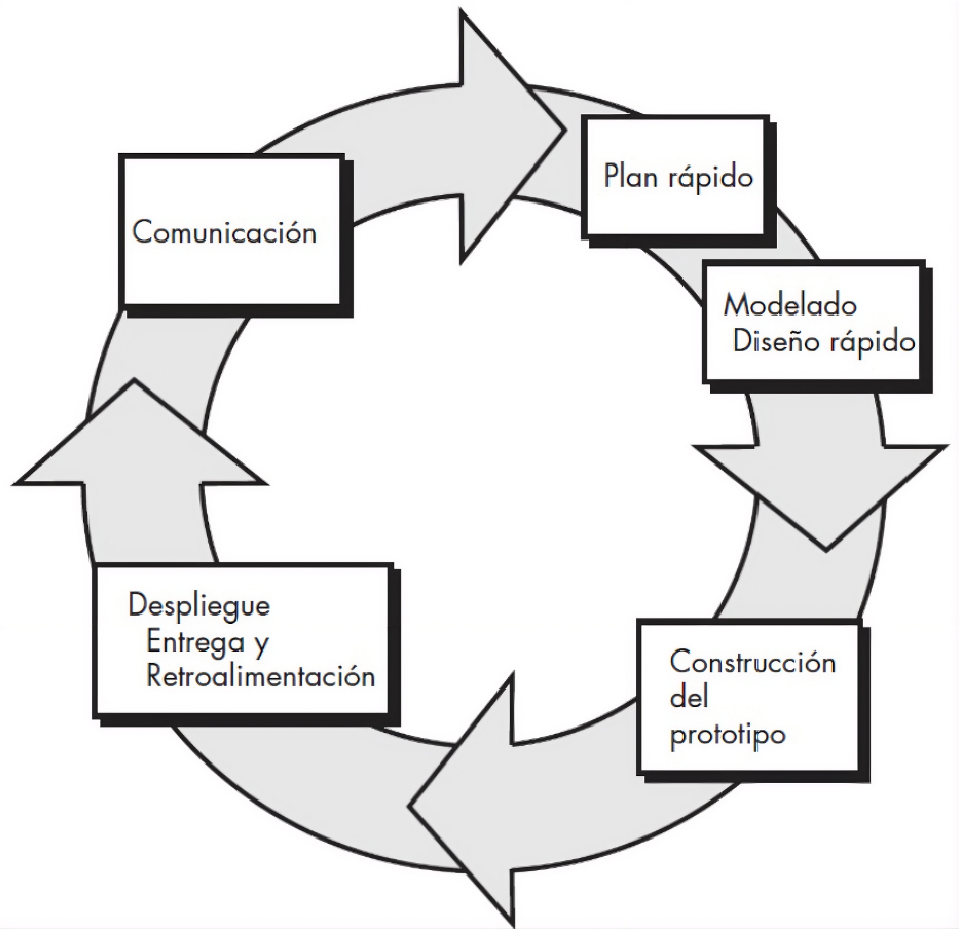
\includegraphics[width=0.70\textwidth]{fig_paradigma_prototipos}
    \caption{Paradigma de Construcción de Prototipos.}
    \label{fig:paradigma_prototipos}
\end{figure}

% ──────────────────────────────────────────────────────────
\subsection{Justificación del Enfoque Evolutivo}
\label{ssec:justificacion_evolutivo}

La elección del prototipado evolutivo sobre modelos secuenciales como el modelo en cascada
responde a la naturaleza del proyecto: un simulador interactivo con alta complejidad
algorítmica y visual, cuyos requisitos didácticos solo pueden validarse con usuarios
reales~\cite{pressman2020}. Las ventajas concretas para AUTECH son:

\textbf{Reducción de riesgos técnicos.} Validar el motor gráfico y la lógica de validación
de cadenas en modelos simples como los autómatas finitos antes de abordar arquitecturas más
complejas como las Máquinas de Turing reduce significativamente la probabilidad de errores
estructurales en etapas avanzadas~\cite{aho2006, pressman2020}.

\textbf{Adaptabilidad didáctica.} Evaluar la retención y usabilidad del estudiante en las
primeras etapas permite calibrar la dificultad de los niveles y los componentes de
ludificación con datos reales, en lugar de suposiciones
iniciales~\cite{deterding2011, nielsen1994}.

\textbf{Entrega temprana de valor.} Cada ciclo produce un módulo funcional que puede probarse
en el entorno académico real, sin necesidad de esperar a que el sistema esté
completo~\cite{escom2016}.

Este principio se evidencia en la propia evolución del proyecto: durante el primer ciclo de
desarrollo, la arquitectura y el stack tecnológico definidos en el protocolo inicial fueron
refinados como resultado directo de la validación técnica. El prototipado evolutivo no solo
permite, sino que anticipa este tipo de ajustes: cada ciclo aporta información real que orienta
las decisiones del siguiente, haciendo del cambio controlado una fortaleza del paradigma, sin
desviarnos completamente de él~\cite{pressman2010}.

% ──────────────────────────────────────────────────────────
\subsection{Definición de los Ciclos de Iteración}
\label{ssec:ciclos}

El proyecto se estructura en tres ciclos de desarrollo, cada uno escalando progresivamente en
complejidad teórica y funcionalidad operativa:

\textbf{Ciclo~0: Núcleo y Lenguajes Regulares.} Construcción de la arquitectura base bajo un
esquema de Layered Architecture con estructura modular por funcionalidad. Incluye el motor de
simulación para Autómatas Finitos Deterministas y No Deterministas, las validaciones lógicas
de cadenas, además de la simulación de Autómatas de pila y la gestión inicial de usuarios
mediante Supabase~\cite{pressman2020, supabase2024}. En este ciclo solo se incluyen pruebas
internas que no consideran la validación con estudiantes y/o profesores, debido a que aún no
estaría implementado por completo el módulo de gestión y estadísticas.

\textbf{Ciclo~1: Gestión Docente.} Se integra el panel de analíticas en aplicación desktop
para el docente, con visualización semaforizada del desempeño grupal e
individual~\cite{materialdesign2023}. Refinación del prototipo anterior basado en validaciones
con estudiantes y profesores. Y se integra en panel del simulador, la opción de conversión de
un autómata pila a su gramática independiente del contexto equivalente.

\textbf{Ludificación Avanzada:} Consolidación del ecosistema completo. Se despliega el
sistema de insignias y rachas para fortalecer la autonomía y retención del
estudiante~\cite{deterding2011}. Refinación del prototipo anterior basado en validaciones con
estudiantes y profesores, además de los manuales correspondientes.

\textbf{Ciclo~2:} Se integra al simulador la opción de simulación de máquinas de Turing
unicinta, así como las opciones de operaciones sobre lenguajes regulares, conversión de
AFN, AFN-$\varepsilon$ a AFD, y minimización de estados, e integra las notificaciones de
estilo push.

% ──────────────────────────────────────────────────────────
\subsection{Cronograma de actividades}
\label{ssec:cronograma}

\begin{table}[H]
    \centering
    \caption{Cronograma de actividades generales para cada ciclo de desarrollo.}
    \label{tab:cronograma}
    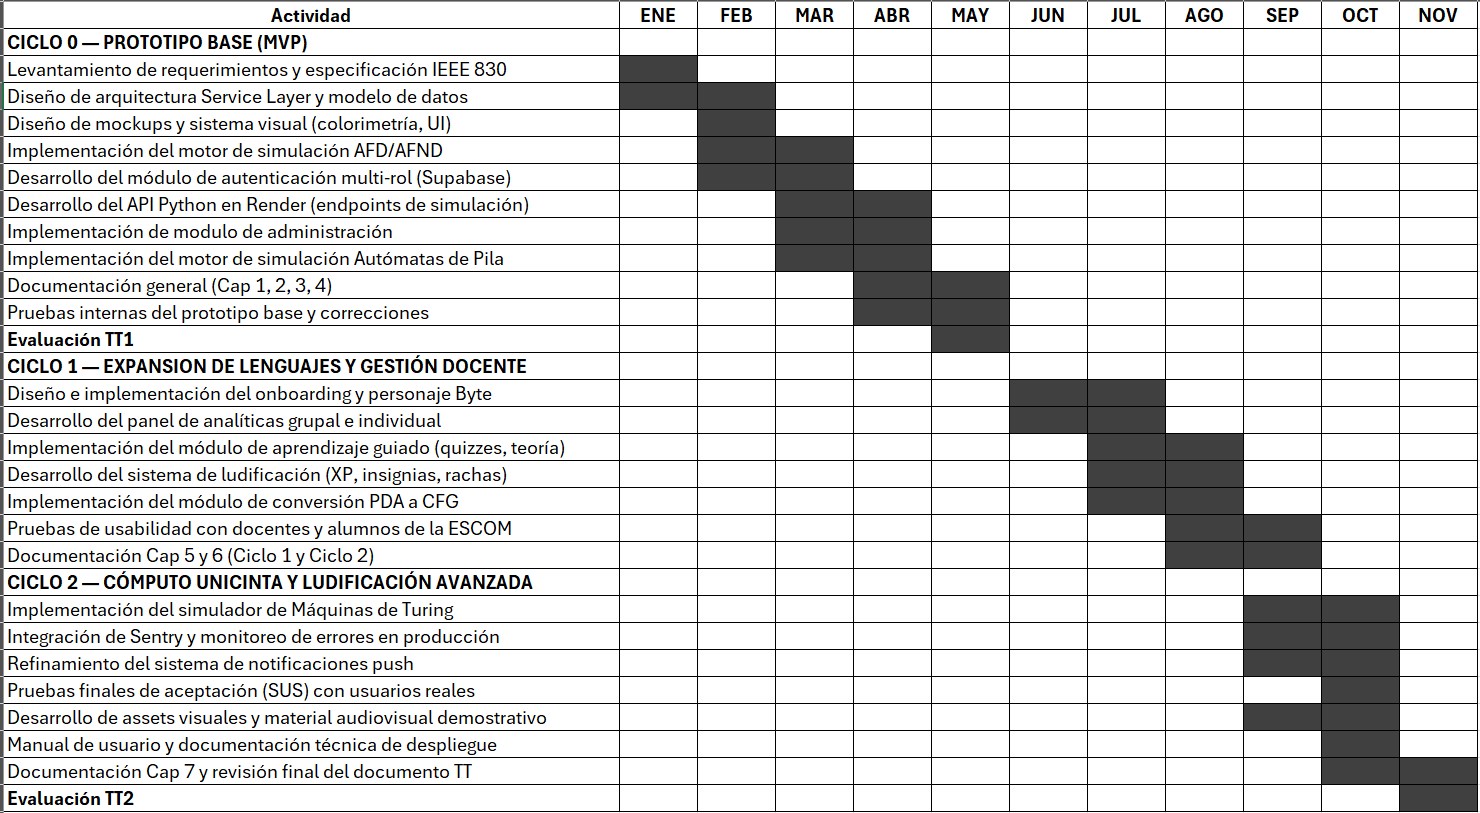
\includegraphics[width=\textwidth]{tabla_cronograma}
\end{table}

% ─────────────────────────────────────────────────────────────
\section{Objetivos}
\label{sec:objetivos}

\subsection{Objetivo General}
\label{ssec:obj_general}

Diseñar e implementar una plataforma educativa móvil ludificada para Android que permita a los
estudiantes de Teoría de la Computación de la ESCOM simular, construir y validar modelos
computacionales de la Jerarquía de Chomsky \cite{church1936}, cuya base teórica formal
fue establecida por Turing \cite{turing1936}, además de contar con un sistema de aprendizaje
guiado por niveles, analíticas de desempeño para el docente y soporte multi-rol.

\subsection{Objetivos Específicos}
\label{ssec:obj_especificos}

\begin{itemize}
    \item Implementar un motor de simulación gráfica interactiva que permita la construcción,
        manipulación táctil y validación de modelos computacionales, incluyendo conversiones
        automáticas entre modelos equivalentes.

    \item Diseñar un sistema de aprendizaje guiado con progresión por niveles, integrando
        teoría, ejercicios prácticos y retroalimentación inmediata para el estudiante.

    \item Desarrollar un panel de a nalíticas en desktop orientado al perfil docente, capaz de
        procesar y visualizar métricas de desempeño grupal e individual mediante indicadores
        semaforizados.

    \item Integrar un mecanismo de persistencia y sincronización de datos en la nube mediante
        Supabase, que garantice el funcionamiento de la aplicación en entornos sin conexión y
        salvaguarde el progreso académico~\cite{supabase2024}.

    \item Construir un módulo de administración global para la gestión centralizada de usuarios
        y control de acceso al sistema.
\end{itemize}

% ─────────────────────────────────────────────────────────────
\section{Justificación}
\label{sec:justificacion}

El desarrollo de AUTECH responde a la necesidad de modernizar las herramientas didácticas
disponibles para la asignatura de Teoría de la Computación en la ESCOM, abordando la
problemática desde tres dimensiones: la eficiencia académica, la accesibilidad tecnológica y
la alineación institucional.

\subsection{Justificación Académica}
\label{ssec:just_academica}

La Teoría de la Computación es base obligada para materias de alto rigor técnico en semestres
superiores, como el diseño de compiladores y la arquitectura de
computadoras~\cite{ipn2020, aho2006}. La asimilación superficial de sus conceptos llega a
generar un fenómeno de arrastre de deficiencias que compromete la trayectoria del estudiante:
al existir una dependencia seriada de conocimientos, la falta de comprensión en esta materia
frena el avance y puede derivar en índices más altos de recurse en ciertas materias, lo que a
su vez en ocasiones llega a saturar la oferta educativa~\cite{tinto1987}.

Un factor que hace que esta problemática sea más difícil de afrontar es que los métodos de
enseñanza tradicionales, centrados en la pizarra y los apuntes, privilegian un único canal de
transmisión del conocimiento. Sin embargo, los estudiantes no aprenden de forma homogénea:
el modelo VARK identifica perfiles de aprendizaje visual, auditivo, lector/escritor y
kinestésico, cuyas necesidades cognitivas difieren significativamente entre
sí~\cite{fleming1992}. En un entorno donde la herramienta principal es JFLAP ---una interfaz
estática operada desde escritorio---, los estudiantes kinestésicos y visuales, que requieren
manipulación directa y representaciones dinámicas para consolidar conceptos abstractos, se
encuentran en desventaja sistemática~\cite{felder2016}.

AUTECH atiende esta brecha mediante un diseño multimodal: la construcción táctil de autómatas
responde al perfil kinestésico, las animaciones y diagramas dinámicos al perfil visual, y el
contenido teórico estructurado por lección al perfil lector. Como trabajo futuro, está
considerada la implementación de elementos de sonido para incluir los perfiles de aprendizaje
auditivos junto con el material audiovisual, sin olvidar los elementos hápticos que pueden ser
considerados de ser necesario después del ciclo~1. Esta convergencia de canales no busca validar
empíricamente los estilos de aprendizaje, sino reducir la dependencia de un único modo de
transmisión del conocimiento y ampliar el alcance didáctico de la
herramienta~\cite{felder2016, sweller1988}.

\subsection{Justificación Tecnológica y de Movilidad}
\label{ssec:just_tecnologica}

Aunque la comunidad estudiantil de la ESCOM tiene acceso a equipos de cómputo, la dependencia
de software de escritorio como JFLAP restringe el estudio a entornos fijos y sesiones de
laboratorio programadas~\cite{rodger2006}. En un contexto donde un sector considerable de los
estudiantes invierte hasta cinco horas diarias en traslados metropolitanos, la portabilidad se
convierte en un factor relacionado con el rendimiento académico~\cite{kukulska2007}. AUTECH
permite convertir esos tiempos muertos en sesiones de práctica activa, aprovechando la
disponibilidad del dispositivo móvil y mitigando además los problemas de conectividad mediante
su modo sin conexión~\cite{crompton2018, materialdesign2023}.

\subsection{Justificación Institucional}
\label{ssec:just_institucional}

El Instituto Politécnico Nacional promueve activamente la incorporación de tecnologías que
modernicen y dinamicen sus procesos educativos a través del modelo educativo del IPN, así como
el documento rector de operación y evaluación para los trabajos terminales. Sin embargo, con
frecuencia existe una brecha entre los objetivos del programa de estudios y las herramientas
realmente disponibles en el aula~\cite{ipn2020, escom2016}. AUTECH se alinea con esa visión
institucional al ofrecer una solución tecnológica original, desarrollada desde la propia
comunidad de la ESCOM, que responde a las necesidades concretas de sus estudiantes y docentes.

% ─────────────────────────────────────────────────────────────
\section{Resultados Esperados}
\label{sec:resultados}

Al concluir el desarrollo e implementación del proyecto, se proyecta la obtención de los
siguientes resultados tangibles y medibles, orientados a satisfacer las necesidades de
actualización tecnológica en la Academia de Ciencias de la Computación de la
ESCOM~\cite{ipn2020, escom2016}.

\subsection{Ecosistema de Software Funcional}
\label{ssec:ecosistema}

\begin{itemize}
    \item \textbf{Aplicación Móvil (AUTECH):} Un paquete de instalación (.APK) para el
        sistema operativo Android que integre el motor de simulación de autómatas, el módulo
        de aprendizaje guiado y el validador algorítmico de lenguajes formales, además de los
        módulos anteriormente mencionados~\cite{crompton2018}.

    \item \textbf{Panel de Gestión en aplicación de escritorio (Dashboard):} Una plataforma
        administrativa para el cuerpo docente que, mediante Supabase como infraestructura de
        base de datos relacional en la nube, permita visualizar de forma centralizada las
        métricas de desempeño grupal e individual de múltiples grupos y/o carreras de la
        ESCOM~\cite{supabase2024}.
\end{itemize}

\subsection{Métricas de Éxito y Validación Didáctica}
\label{ssec:metricas}

El impacto del proyecto no se medirá basándose en índices de aprobación externos, sino a
través de la evaluación directa del software mediante instrumentos estandarizados:

\begin{itemize}
    \item \textbf{Validación de Usabilidad:} Obtención de un puntaje superior al 80\% de
        aceptación en la Escala de Usabilidad del Sistema (SUS) aplicada a una muestra
        representativa de estudiantes activos y consideración de un modelo TAM~\cite{brooke1996}
        para los ciclos~1 y~2.

    \item \textbf{Autopercepción de Competencias:} Confirmación, mediante instrumentos de
        evaluación post-uso, de una reducción en la carga cognitiva y un aumento en la
        confianza técnica de los usuarios al modelar los componentes específicos de la
        Jerarquía de Chomsky~\cite{hopcroft2007, sweller1988}.

    \item \textbf{Analíticas de Intervención:} Generación de un registro histórico (o al
        menos con un historial de 3~semestres) en la nube que mapee los errores lógicos más
        frecuentes por grupo, dotando al docente de datos empíricos para realizar
        intervenciones didácticas de precisión~\cite{felder2016}.
\end{itemize}

\subsection{Sistema de Progresión y Ludificación}
\label{ssec:ludificacion}

El componente de ludificación producirá un historial de competencias digitales para cada
usuario, estructurado en los siguientes elementos:

\begin{itemize}
    \item \textbf{Jerarquía de Insignias:} Un sistema de reconocimiento progresivo con
        insignias alusivas a las secciones completadas que clasifica el dominio del estudiante
        a partir de la resolución de problemas y la depuración de cadenas, además de los
        típicos cuestionarios~\cite{deterding2011}.

    \item \textbf{Desbloqueo Secuencial de Mundos:} Evidencia visual del avance lógico del
        alumno a través de los modelos de la Jerarquía de Chomsky, desde los Autómatas
        Finitos hasta las Máquinas de Turing, con la excepción mencionada anteriormente de
        los lenguajes tipo~1~\cite{hopcroft2007}.

    \item \textbf{Indicador de Racha:} Registro visual del número de días consecutivos en
        que el alumno ha completado ejercicios, fomentando la práctica continua y la
        constancia en el estudio.
\end{itemize}

\subsection{Interoperabilidad y Transferencia Tecnológica}
\label{ssec:interoperabilidad}

\textbf{Compatibilidad con JFLAP y FSAM:} Desarrollo de un módulo de análisis (parser) capaz
de importar y exportar la estructura XML de los archivos .jff, garantizando que los autómatas
construidos en el dispositivo móvil sean bidireccionalmente compatibles con el software de
escritorio utilizado en los laboratorios de la institución~\cite{rodger2006}, además de la
implementación de archivos exportados desde FSAM.

\textbf{Documentación de Ingeniería:} Entrega de un repositorio de código fuente organizado
bajo el patrón de Layered Architecture y manuales correspondientes, asegurando que el sistema
sea mantenible y escalable por futuras generaciones de la ESCOM~\cite{pressman2020, reenskaug1979}.

% ─────────────────────────────────────────────────────────────
\section{Restricciones y Fronteras de Diseño}
\label{sec:restricciones}

Para delimitar el alcance técnico y operativo del proyecto AUTECH, y garantizar su viabilidad
dentro de los tiempos de desarrollo del Trabajo Terminal, se establecen las siguientes
fronteras fundamentales:

\subsection{Restricciones Técnicas y de Hardware}
\label{ssec:restricciones_tecnicas}

\textbf{Segmentación de Plataforma:} El desarrollo se orienta de forma exclusiva al sistema
operativo Android, estableciendo la versión 9.0 (Pie, API~28) como requerimiento
mínimo~\cite{google2023android}. No se contempla compatibilidad con iOS debido a los costos
de licenciamiento asociados a la cuenta de desarrollador de Apple, además de la falta de
infraestructura para el empaquetado de recursos para iOS.

\textbf{Optimización Gráfica y Rendimiento:} El motor de renderizado Impeller, utilizado para
la manipulación fluida de autómatas en pantalla, aprovecha Vulkan como backend gráfico
principal cuando el dispositivo lo soporta, manteniéndose compatible mediante OpenGL~ES en
hardware que no cuente con dicha capacidad~\cite{flutter2024a}. El hardware mínimo requerido
consiste en un procesador de arquitectura de 64~bits y 4~GB de memoria RAM.

\textbf{Conectividad Híbrida:} El sistema operará bajo un modelo de tolerancia a
desconexiones. El motor de simulación y las lecciones teóricas funcionarán de manera autónoma
sin conexión a internet. No obstante, se requiere conectividad intermitente para la
autenticación de usuarios, la visualización de material audiovisual externo y la
sincronización de analíticas hacia el panel docente mediante Supabase~\cite{supabase2024}.

\textbf{Adaptabilidad de Interfaz:} El diseño garantizará la correcta visualización en
smartphones convencionales y tablets, priorizando una distribución de elementos que maximice
el área de trabajo del simulador en función del dispositivo del usuario
(responsive)~\cite{materialdesign2023}.

\subsection{Fronteras Didácticas y Operativas}
\label{ssec:fronteras_didacticas}

\textbf{Alcance Temático Institucional:} La base algorítmica y de contenidos se restringe
estrictamente a los tópicos del programa sintético de Teoría de la Computación
(ISC~2020)~\cite{ipn2020}. El avance lógico sigue la Jerarquía de Chomsky, Autómatas Finitos,
Autómatas de Pila y Máquinas de Turing, omitiendo deliberadamente temas de complejidad
computacional avanzada, como las clases P vs.\ NP, que exceden el propósito de esta
herramienta~\cite{hopcroft2007}, así como los lenguajes tipo~1 dentro de la Jerarquía de
Chomsky.

\textbf{Rol de Evaluación:} AUTECH está creada como una plataforma de refuerzo y evaluación
formativa. El software no pretende sustituir el proceso de evaluación sumativa oficial del
docente titular de la asignatura, sino tomar el rol de herramienta de apoyo a las clases
impartidas por el mismo~\cite{escom2016}.

\textbf{Estrategia Multimedia:} El contenido de video se define como recurso secundario. Las
lecciones están diseñadas para asimilarse íntegramente mediante textos, autómatas interactivos
e infografías, asegurando que la falta de ancho de banda no comprometa la integridad
didáctica de la unidad~\cite{crompton2018}.
\chapter{Marco Teórico}
\label{ch:marco_teorico}

Este capítulo contendrá los fundamentos de autómatas, lenguajes formales y gramáticas.
\vspace*{-4cm}
\chapter{Análisis}
\label{ch:analisis}

En este capítulo se presenta el desglose formal de las necesidades del sistema AUTECH mediante la especificación de sus requerimientos funcionales y no funcionales, el establecimiento de sus reglas de negocio, y el modelado detallado de sus casos de uso bajo el estándar UML.

\section{Requerimientos Globales del Sistema (IEEE 830)}
\label{sec:ieee830}

La especificación de requisitos se fundamenta en la norma IEEE Std 830-1998, asegurando una trazabilidad bidireccional y una comunicación sin ambigüedades entre la arquitectura de software y las necesidades didácticas institucionales \cite{ieee1998}.

\subsection{Requerimientos Funcionales}
\label{subsec:req_funcionales}

Los requerimientos funcionales (RF) definen el comportamiento interno del sistema, las transformaciones de datos y los servicios directos que se proveen a los distintos perfiles de usuario. Para garantizar la cohesión del diseño, se han classified en cuatro módulos arquitectónicos, como se definen en la Tabla~\ref{tab:rf_sistema} y la Tabla~\ref{tab:rf_sistema_p2}.

\begin{table}[htbp]
    \centering
    \small
    \caption{Requerimientos Funcionales del Sistema AUTECH, organizados en cuatro módulos: Gestión y Seguridad (RF-01 a RF-03), Simulación y Motor Algorítmico (RF-04 a RF-08), Didáctico y de Ludificación (RF-09 a RF-12) e Interoperabilidad y UX (RF-13 a RF-15).}
    \label{tab:rf_sistema}
    \begin{tabular}{l l p{9.5cm}}
        \toprule
        \textbf{ID} & \textbf{Nombre del Requerimiento} & \textbf{Especificación Técnica} \\
        \midrule
        \multicolumn{3}{l}{\textbf{MÓDULO DE GESTIÓN Y SEGURIDAD}} \\
        \midrule
        RF-01 & Gestión Multi-Rol & Administrar el control de acceso de manera multiplataforma y concurrente para tres perfiles jerárquicos: Administrador (gestión global), Docente (gestión académica) y Alumno (simulación) \cite{pressman2020}. \\
        \addlinespace
        RF-02 & Aprovisionamiento Docente & Permitir el envío de solicitudes de registro docente. Tras la validación del Administrador (vía entorno desktop o móvil), el sistema deberá aprovisionar la cuenta automatizando el envío de credenciales temporales vía correo electrónico. \\
        \addlinespace
        RF-03 & Gestión de Grupos Académicos & Proveer al perfil Docente de un panel de control disponible en plataformas desktop y móvil para crear, modificar o eliminar grupos, así como generar identificadores alfanuméricos (códigos de invitación) para el enrolamiento de alumnos \cite{escom2016}. \\
        \midrule
        \multicolumn{3}{l}{\textbf{MÓDULO DE SIMULACIÓN Y MOTOR ALGORÍTMICO}} \\
        \midrule
        RF-04 & Editor de Autómatas Finitos & Desplegar un canvas interactivo en la aplicación móvil que permita la construcción y edición topológica de Autómatas Finitos Deterministas (AFD) y No Deterministas (AFND) \cite{ipn2020}. \\
        \addlinespace
        RF-05 & Editor de Autómatas de Pila & Proveer herramientas de diseño para Autómatas de Pila (AP) en la interfaz móvil, integrando la declaración del alfabeto de la pila ($\Gamma$) y la gestión de transiciones no deterministas \cite{hopcroft2007}. \\
        \addlinespace
        RF-06 & Editor de Máquinas de Turing & Desplegar en la aplicación móvil un simulador de Máquina de Turing (MT) orientado a la función de reconocimiento de lenguajes, incorporando una cinta infinita visual y control de cabezal bidireccional \cite{sipser2012}. \\
        \addlinespace
        RF-07 & Validador Lógico Multinivel & Ejecutar la validación algorítmica de cadenas de entrada en tres modalidades asíncronas: 1) Ejecución paso a paso, 2) Resolución de clausuras épsilon ($\epsilon$), y 3) Evaluación masiva de baterías de prueba (\textit{Bulk Test}) \cite{sinchi2018}. \\
        \addlinespace
        RF-08 & Transformación Algorítmica & Ejecutar conversiones matemáticas automatizadas, incluyendo: transformación de AFND a AFD, minimización de estados equivalentes y conversión bidireccional entre Expresiones Regulares y grafos \cite{kelley2001}. \\
        \bottomrule
    \end{tabular}
\end{table}

\begin{table}[htbp]
    \centering
    \small
    \caption{Requerimientos Funcionales del Sistema AUTECH (Continuación).}
    \label{tab:rf_sistema_p2}
    \begin{tabular}{l l p{9.5cm}}
        \toprule
        \textbf{ID} & \textbf{Nombre del Requerimiento} & \textbf{Especificación Técnica} \\
        \midrule
        \multicolumn{3}{l}{\textbf{MÓDULO DIDÁCTICO Y DE LUDIFICACIÓN}} \\
        \midrule
        RF-09 & Evaluaciones Teóricas (Quizzes) & Permitir la creación y asignación multiplataforma de reactivos de opción múltiple orientados exclusivamente a la validación de fundamentos teóricos de la asignatura \cite{felder2016}. \\
        \addlinespace
        RF-10 & Analítica de Desempeño Docente & Procesar las métricas de uso y generar visualizaciones estadísticas (indicadores semaforizados) del avance grupal e individual (aciertos, errores frecuentes y completitud temporal) accesibles para el profesor \cite{munoz2012}. \\
        \addlinespace
        RF-11 & Ecosistema de Ludificación & Orquestar el progreso del usuario mediante el bloqueo/desbloqueo de ``mundos'' basados en la Jerarquía de Chomsky, calculando puntos de experiencia (XP) y gestionando contadores de racha de estudio en la app móvil del Alumno \cite{deterding2011}. \\
        \addlinespace
        RF-12 & Integración Multimedia & Integrar y reproducir material audiovisual de refuerzo desde fuentes externas de manera adaptativa en la interfaz móvil \cite{crompton2018}. \\
        \midrule
        \multicolumn{3}{l}{\textbf{MÓDULO DE INTEROPERABILIDAD Y UX}} \\
        \midrule
        RF-13 & Interoperabilidad de Estructuras & Soportar la importación y exportación bidireccional del mapeo de grafos utilizando los esquemas XML estándar de la industria académica: \texttt{.jff} (JFLAP) y \texttt{.fsam} a través del gestor de archivos nativo de cada entorno \cite{rodger2006}. \\
        \addlinespace
        RF-14 & Asistente de Inducción (Onboarding) & Desplegar una secuencia de instrucciones superpuestas e interactivas al detectar el primer inicio de sesión en la aplicación móvil del Alumno, con capacidad de ser omitida por el usuario \cite{materialdesign2023}. \\
        \addlinespace
        RF-15 & Modo de Práctica Autónoma & Habilitar el acceso irrestricto en la app móvil a los módulos de simulación y lecciones teóricas para cuentas de Alumno que no estén vinculadas a un código de grupo docente \cite{nielsen1994}. \\
        \bottomrule
    \end{tabular}
\end{table}

\newpage
\subsection{Requerimientos No Funcionales (RNF)}
\label{subsec:req_no_funcionales}

Los requerimientos no funcionales (RNF) especifican las restricciones técnicas, criterios de calidad del sistema, directrices de seguridad y métricas de rendimiento indispensables para garantizar el correcto funcionamiento transversal de la arquitectura de AUTECH, detallados en la Tabla~\ref{tab:req_no_funcionales}.

\begin{table}[htbp]
    \centering
    \small
    \caption{Especificación de Requerimientos No Funcionales del Ecosistema AUTECH.}
    \label{tab:req_no_funcionales}
    \begin{tabular}{l l p{9.5cm}}
        \toprule
        \textbf{ID} & \textbf{Atributo de Calidad} & \textbf{Especificación y Restricción Técnica} \\
        \midrule
        RNF-01 & Rendimiento Gráfico & El renderizado y la animación matemática de los grafos sobre el canvas interactivo en Flutter debe mantener una tasa de refresco estable de 60 FPS tanto en dispositivos móviles como en entornos Desktop (Windows/macOS) \cite{flutter2024a}. \\
        \addlinespace
        RNF-02 & Persistencia Local Móvil & La lectura y escritura de estructuras de autómatas y progreso local en la aplicación móvil del Alumno debe realizarse mediante cajas no relacionales de Hive, garantizando tiempos de respuesta inferiores a los 15 ms. \\
        \addlinespace
        RNF-03 & Resiliencia Offline & El cliente móvil del Alumno debe procesar el cambio dinámico de red mediante un Service Layer reactivo, encolando localmente las peticiones de sincronización en background al perder de forma temporal la conectividad \cite{flutter2024c}. \\
        \addlinespace
        RNF-04 & Disponibilidad de API & La API de servicios web desplegada en la infraestructura en la nube de Render debe responder eficientemente a las peticiones concurrentes de las aplicaciones, garantizando un \textit{uptime} del 99.5\% anual. \\
        \addlinespace
        RNF-05 & Seguridad y Cifrado & Todo flujo de datos e intercambio de información entre los clientes de software (móviles o desktop) y la base de datos centralizada debe realizarse obligatoriamente mediante peticiones cifradas bajo el protocolo HTTPS (TLS 1.3). \\
        \addlinespace
        RNF-06 & Seguridad en Capa de Datos & El acceso a la persistencia en la nube debe controlarse estrictamente a través de políticas de seguridad a nivel de fila (RLS, \textit{Row Level Security}) vinculadas al ID único de usuario de la sesión activa en cualquier plataforma \cite{supabase2024}. \\
        \addlinespace
        RNF-07 & Escalabilidad Concurrente & El esquema de base de datos relacional y el pool de conexiones del backend deben estar dimensionados para soportar consultas simultáneas provenientes de múltiples peticiones concurrentes en periodos de evaluación masiva bajo estándares internacionales de calidad \cite{iso2011}. \\
        \bottomrule
    \end{tabular}
\end{table}

\clearpage
\section{Reglas de Negocio}
\label{sec:reglas_negocio}

Las reglas de negocio definen las políticas, restricciones lógicas y leyes matemáticas constantes, que el sistema debe respetar durante su ejecución. A diferencia de los requerimientos funcionales, estas reglas aseguran que la simulación gráfica sea matemáticamente exacta y que el avance del estudiante sea didácticamente coherente con el programa de estudios \cite{ipn2020, hopcroft2007}. La especificación detallada de estas directrices se presenta en la Tabla~\ref{tab:reglas_negocio}.

\begin{table}[htbp]
    \centering
    \small
    \caption{Reglas de Negocio del Sistema AUTECH.}
    \label{tab:reglas_negocio}
    \begin{tabular}{l l p{9.5cm}}
        \toprule
        \textbf{ID} & \textbf{Nombre de la Regla} & \textbf{Restricción Lógica y Matemática} \\
        \midrule
        RN-01 & Determinismo Estricto (AFD) & Durante la edición de un Autómata Finito Determinista, el sistema impedirá la ejecución de la simulación y desplegará una alerta de error si detecta que un estado posee múltiples transiciones de salida evaluadas con el mismo símbolo del alfabeto \cite{hopcroft2007}. \\
        \addlinespace
        RN-02 & Integridad de Memoria LIFO & En el simulador de Autómatas de Pila, el motor de validación prohibirá cualquier operation de extracción (POP) si el estado actual de la pila contiene únicamente el símbolo de fondo inicial ($Z_0$), evitando desbordamientos lógicos \cite{hopcroft2007}. \\
        \addlinespace
        RN-03 & Límite Físico de Cinta (MT) & Conforme al modelo estándar de Máquina de Turing de cinta semi-infinita, el sistema restringirá el desplazamiento del cabezal hacia la izquierda si su posición actual corresponde a la celda de inicio (índice cero) \cite{hopcroft2007}. \\
        \addlinespace
        RN-04 & Umbral de Competencia Didáctica & El sistema aplicará un candado lógico que impedirá el desbloqueo de un nivel superior (por ejemplo, la transición de Lenguajes Regulares a Libres de Contexto) a menos que el usuario acredite el módulo vigente con un puntaje mínimo aprobatorio de 80/100. La implementación de esta regla corresponde al Ciclo 1 del prototipado evolutivo, una vez que el sistema de progresión base quede consolidado en el Ciclo 0 \cite{ipn2020}. \\
        \addlinespace
        RN-05 & Límite de Complejidad Topológica & Para mantener el alineamiento con el RNF-01 de rendimiento, el lienzo de simulación emitirá una advertencia preventiva de optimización si la topología del grafo diseñado por el usuario alcanza los 15 estados activos. \\
        \addlinespace
        RN-06 & Iteración Formativa Ilimitada & El sistema garantizará que las cuentas con rol de Alumno posean intentos infinitos para la resolución de simulaciones y cuestionarios teóricos, priorizando la internalización del conocimiento por repetición sobre la penalización punitiva. \\
        \bottomrule
    \end{tabular}
\end{table}

\clearpage 

\section{Especificación de Requisitos y Modelado Funcional (UML)}
\label{sec:especificacion_uml}

La ingeniería de requisitos visual permite modelar las limitaciones operativas del sistema, facilitando la comprensión de los flujos de trabajo sin comprometerse con detalles de implementación a nivel de código. Para mantener el rigor técnico exigido en el IPN, se utiliza el estándar industrial UML 2.5 (Lenguaje de Modelado Unificado), el cual esquematiza cómo las entidades humanas interactúan con los procesos de la Jerarquía de Chomsky y el motor analítico del sistema \cite{pressman2020}.

\subsection{Actores del Sistema}
\label{subsec:actores_sistema}

De acuerdo con las especificaciones de UML 2.5, un ``Actor'' representa un rol que desempeña un usuario humano o un sistema externo al interactuar con el caso de uso \cite{pressman2020}. Para AUTECH, se han definido estrictamente tres perfiles jerárquicos basados en una arquitectura de control de acceso por roles (RBAC) \cite{supabase2024}.

\begin{quote}
    \small \textit{\textbf{Nota Técnica de Arquitectura:} Se omite deliberadamente la inclusión de componentes de infraestructura interna, como la base de datos local Hive o el proveedor de autenticación Supabase Auth, ya que no inician interacciones de forma autónoma, sino que responden a peticiones del cliente.}
\end{quote}

\begin{description}
    \item[\textbf{Alumno (Actor Primario - Móvil):}] Estudiante matriculado en la ESCOM. Su objetivo principal es interactuar exclusivamente con el cliente móvil (Android) para resolver simulaciones de autómatas, consultar teoría algorítmica y gestionar su progresión académica dentro del ecosistema ludificado \cite{ipn2020, materialdesign2023}.
    \item[\textbf{Docente (Actor Primario - Multiplataforma adaptativo Desktop/Móvil):}] Profesor titular de la asignatura de Teoría de la Computación. Su interacción se centraliza en el Dashboard Desktop y dispositivos móviles, donde ejerce funciones de evaluación formativa, gestión de grupos académicos (códigos de invitación) y análisis de métricas de desempeño \cite{felder2016}.
    \item[\textbf{Administrador (Actor Secundario - Multiplataforma adaptativo Desktop/Móvil):}] Perfil técnico y operativo con privilegios globales (\textit{Super User}). Su responsabilidad recae en el aprovisionamiento de cuentas institucionales (validación y aprobación de registros docentes) y el mantenimiento de los parámetros de configuración globales del sistema \cite{supabase2024}.
\end{description}
\subsection{Casos de Uso}
\label{subsec:casos_uso}

El catálogo de Casos de Uso (CU) define las interacciones entre los actores (Alumno, Docente, Administrador) y los servicios del sistema, clasificando cada función por su importancia para el proceso educativo (Prioridad) y su impacto en la estabilidad del software (Criticidad). Los casos de uso se derivan de las funcionalidades implementadas en Flutter/Dart utilizando Supabase como plataforma de servicios backend.

Para optimizar la trazabilidad y ofrecer una visión holística del sistema, el catálogo completo de AUTECH se ha unificado en la Tabla~\ref{tab:catalogo_cu_consolidado} y la Tabla~\ref{tab:catalogo_cu_consolidado_p2}, segmentado jerárquicamente por el ámbito de aplicación de cada módulo y ordenado en una secuencia numérica progresiva continua.

\begin{table}[htbp]
    \centering
    \small
    \caption{Catálogo Consolidado de Casos de Uso del Ecosistema AUTECH (Parte 1).}
    \label{tab:catalogo_cu_consolidado}
    \begin{tabular}{l p{5.5cm} l l l}
        \toprule
        \textbf{Código} & \textbf{Caso de Uso} & \textbf{Actor} & \textbf{Prioridad} & \textbf{Criticidad} \\
        \midrule
        \multicolumn{5}{l}{\textbf{I. MÓDULO DE AUTENTICACIÓN, SEGURIDAD Y ACCESOS (Transversal)}} \\
        \midrule
        CU-01 & Iniciar Sesión Alumno & Alumno & CRÍTICA & Bloqueante \\
        CU-02 & Registrarse Alumno & Alumno & Alta & Bloqueante \\
        CU-03 & Iniciar Sesión Docente/Admin & Docente/Admin & CRÍTICA & Bloqueante \\
        CU-04 & Solicitar Registro Docente & Docente & Alta & Alta \\
        CU-05 & Recuperar Contraseña & Alumno/Docente & Media & Alta \\
        CU-06 & Cerrar Sesión & Todos & Media & Alta \\
        \midrule
        \multicolumn{5}{l}{\textbf{II. NÚCLEO DE SIMULACIÓN, ALGORITMOS Y APRENDIZAJE (Alumno)}} \\
        \midrule
        \multicolumn{5}{l}{\textit{A. Entorno Interactivo y Motores de Simulación}} \\
        CU-07 & Grafo del Autómata Interactivo & Alumno/Docente & CRÍTICA & Core \\
        CU-08 & Simulación Paso a Paso (Animada) & Alumno & CRÍTICA & Core \\
        CU-09 & Definir, visualizar y simular un PDA & Alumno & Alta & Media \\
        CU-10 & Simulación completa con cinta animada (MT) & Alumno & Alta & Media \\
        \addlinespace
        \multicolumn{5}{l}{\textit{B. Algoritmos de Conversión y Procesamiento Formal}} \\
        CU-11 & Operaciones sobre Lenguajes Regulares & Alumno & Alta & Técnica \\
        CU-12 & Conversión de ER a Autómata & Alumno & Alta & Técnica \\
        CU-13 & Conversión de AFN-$\epsilon$ a AFD & Alumno & CRÍTICA & Algorítmica \\
        CU-14 & Reducción de Estados (Minimización de AFD) & Alumno & Alta & Técnica \\
        CU-15 & Convierte a Gramática Libre de Contexto (CFG) & Alumno & Media & Técnica \\
        \addlinespace
        \multicolumn{5}{l}{\textit{C. Sistema de Evaluación de Retos}} \\
        CU-16 & Ver Retos Disponibles & Alumno & CRÍTICA & Core \\
        CU-17 & Resolver Reto de Simulación & Alumno & CRÍTICA & Core \\
        CU-18 & Enviar Respuesta para Evaluación & Alumno & CRÍTICA & Core \\
        CU-19 & Ver Historial de Respuestas & Alumno & Media & Alta \\
        \midrule
        \multicolumn{5}{l}{\textbf{III. MÓDULO MÓVIL: SINCRONIZACIÓN Y PERSISTENCIA (Arquitectura Offline)}} \\
        \midrule
        CU-20 & Descargar Contenido Teórico (Unidades 1-8) & Alumno & Alta & Alta \\
        CU-21 & Modo Autónomo Offline (Persistencia en Hive) & Alumno & Alta & Alta \\
        CU-22 & Sincronizar Datos con la Nube (API / Supabase) & Alumno & Alta & Alta \\
        \bottomrule
    \end{tabular}
\end{table}

\begin{table}[htbp]
    \centering
    \small
    \caption{Catálogo Consolidado de Casos de Uso del Ecosistema AUTECH (Parte 2).}
    \label{tab:catalogo_cu_consolidado_p2}
    \begin{tabular}{l p{5.5cm} l l l}
        \toprule
        \textbf{Código} & \textbf{Caso de Uso} & \textbf{Actor} & \textbf{Prioridad} & \textbf{Criticidad} \\
        \midrule
        \multicolumn{5}{l}{\textbf{IV. MÓDULO MÓVIL: EXPERIENCIA DE USUARIO Y LUDIFICACIÓN (Alumno)}} \\
        \midrule
        CU-23 & Ver Perfil y Estadísticas de Progreso & Alumno & Media & Media \\
        CU-24 & Ver Calificaciones e Historial & Alumno & Alta & Alta \\
        CU-25 & Gestionar Notificaciones Push & Alumno & Media & Media \\
        CU-26 & Reclamar Insignia de Logro & Alumno & Baja & Media \\
        \midrule
        \multicolumn{5}{l}{\textbf{V. MÓDULO WEB: DASHBOARD DE GESTIÓN DOCENTE (Plataforma Desktop)}} \\
        \midrule
        \multicolumn{5}{l}{\textit{A. Gestión de Contenido Académico y Retos}} \\
        CU-27 & Crear Reto/Ejercicio & Docente & CRÍTICA & Core \\
        CU-28 & Editar/Actualizar Reto & Docente & Alta & Alta \\
        CU-29 & Eliminar Reto & Docente & Media & Media \\
        CU-30 & Asignar Reto a Grupo & Docente & CRÍTICA & Core \\
        CU-31 & Gestionar Material de Apoyo & Docente & Media & Media \\
        \addlinespace
        \multicolumn{5}{l}{\textit{B. Evaluación y Analíticas de Desempeño}} \\
        CU-32 & Ver Respuestas Pendientes de Alumnos & Docente & CRÍTICA & Core \\
        CU-33 & Asignar Retroalimentación Personalizada & Docente & Alta & Alta \\
        CU-34 & Observar calificaciones en analíticas & Docente & CRÍTICA & Core \\
        CU-35 & Ver Analíticas de Desempeño Grupal & Docente & Alta & Alta \\
        CU-36 & Exportar Reportes (PDF/Excel) (Ciclo 2) & Docente & Media & Media \\
        \midrule
        \multicolumn{5}{l}{\textbf{VI. MÓDULO WEB: GESTIÓN ADMINISTRATIVA GLOBAL (Consola Admin)}} \\
        \midrule
        CU-37 & Crear/Gestionar Grupos (Vinculación) & Docente/Admin & Media & Media \\
        CU-38 & Vincular Alumnos a Grupo & Docente/Admin & Media & Media \\
        CU-39 & Aprobar/Rechazar Registro de Docentes & Administrador & CRÍTICA & Seguridad \\
        CU-40 & Gestionar Cuentas de Usuario (Admin) & Administrador & Alta & Crítica \\
        CU-41 & Configurar Parámetros de Ludificación & Administrador & Media & Media \\
        CU-42 & Monitorear Logs de Sistema y Errores & Administrador & Media & Técnica \\
        \bottomrule
    \end{tabular}
\end{table}

\clearpage

\subsection{Descripción de Casos de Uso Críticos}
\label{subsec:descripcion_cu_criticos}

A continuación, se describen las especificaciones de comportamiento lógico, procesamiento algebraico y validación de consistencia en tiempo real para los casos de uso fundamentales del ecosistema AUTECH.

\begin{description}
    \item[\textbf{CU-35: Ver Analíticas de Desempeño Grupal}]~\\
    \textbf{Descripción:} El docente accede a una visualización de datos agregados en el Dashboard Desktop generados automáticamente por el sistema.\\
    \textbf{Procesamiento:} El sistema recupera los datos de desempeño de Supabase y genera métricas semaforizadas (Rojo: $< 70\%$, Amarillo: $70\text{--}85\%$, Verde: $> 85\%$) para identificar deficiencias conceptuales en el grupo. No se requiere intervención manual del docente para calcular o asignar puntajes.

    \item[\textbf{CU-07: Grafo del Autómata Interactivo}]~\\
    \textbf{Descripción:} Proporciona al usuario un lienzo digital táctil para el diseño de modelos computacionales mediante nodos (estados) y aristas (transiciones).\\
    \textbf{Lógica:} El sistema gestiona una estructura de datos de grafos donde cada elemento posee propiedades de la $5\text{-tupla}$ o $7\text{-tupla}$. Permite la edición dinámica de alfabetos y la asignación de estados iniciales y de aceptación con validación de integridad en tiempo real.

    \item[\textbf{CU-08: Simulación Paso a Paso (Animada)}]~\\
    \textbf{Descripción:} Anima el recorrido de una cadena sobre el autómata en tiempo real, resaltando el estado actual y las transiciones activas.\\
    \textbf{Interacción:} El usuario puede controlar la velocidad de la simulación o avanzar manualmente (clic por símbolo), facilitando la identificación de fallos lógicos en el diseño del modelo.

    \item[\textbf{CU-11: Operaciones sobre Lenguajes Regulares}]~\\
    \textbf{Descripción:} Permite al usuario realizar operaciones algebraicas (unión, intersección o diferencia) entre dos autómatas.\\
    \textbf{Procesamiento:} El sistema utiliza la Construcción de Producto, donde el conjunto de estados resultante se basa en el producto cartesiano de los estados de los autómatas originales ($Q_1 \times Q_2$).

    \item[\textbf{CU-13: Conversión de AFN-$\epsilon$ a AFD}]~\\
    \textbf{Descripción:} Transforma un modelo no determinista con transiciones vacías en su equivalente determinista único.\\
    \textbf{Procesamiento:} El sistema calcula la $\epsilon$-clausura para identificar los estados alcanzables sin consumo de entrada. Posteriormente, aplica el algoritmo de construcción de subconjuntos para derivar una función de transición unívoca, garantizando la eliminación de la ambigüedad en el flujo de procesamiento.

    \item[\textbf{CU-14: Reducción de Estados (Minimización de AFD)}]~\\
    \textbf{Descripción:} Optimiza la estructura de un AFD eliminando la redundancia para obtener el autómata mínimo equivalente.\\
    \textbf{Lógica:} Implementa el Algoritmo de Hopcroft mediante la partición de estados en clases de equivalencia (distinguibles vs. no distinguibles). El resultado es un modelo más eficiente en términos de memoria y procesamiento.

    \item[\textbf{CU-12: Conversión de ER a Autómata}]~\\
    \textbf{Descripción:} Traduce una Expresión Regular (ER) ingresada por el usuario en un autómata finito equivalente.\\
    \textbf{Lógica:} Utiliza la Construcción de Thompson, generando una estructura de estados y transiciones épsilon que fragmenta la expresión en sus componentes atómicos (unión, concatenación y clausura de Kleene).

    \item[\textbf{CU-09: Definir, visualizar y simular un PDA}]~\\
    \textbf{Descripción:} Permite el diseño y ejecución de autómatas que utilizan una memoria externa tipo LIFO.\\
    \textbf{Visualización:} El simulador renderiza una pila dinámica donde el usuario observa gráficamente las operaciones de \textit{push} y \textit{pop} conforme se procesan los símbolos de entrada y los símbolos de la cima de la pila.

    \item[\textbf{CU-15: Convierte a Gramática Libre de Contexto (CFG)}]~\\
    \textbf{Descripción:} Genera el conjunto de reglas de producción gramaticales a partir de un autómata de pila o un autómata finito.\\
    \textbf{Resultado:} El sistema extrae las variables, terminales y producciones, permitiendo al alumno visualizar la correspondencia entre el modelo de reconocimiento (autómata) y el modelo generativo (gramática).

    \item[\textbf{CU-10: Simulación completa con cinta animada (MT)}]~\\
    \textbf{Descripción:} Ejecuta el modelo universal de cómputo sobre una cinta de longitud infinita.\\
    \textbf{Componentes:} El sistema anima el movimiento de la cabeza lectora-escritora (izquierda/derecha) y la edición de símbolos en la cinta, permitiendo al alumno validar algoritmos complejos y funciones aritméticas en un entorno visualmente intuitivo.
\end{description}

\section{Diseño del Modelo de Datos}
\label{sec:modelo_datos}

Para garantizar la integridad referencial, la escalabilidad concurrente y el correcto funcionamiento de las políticas de seguridad a nivel de fila (RLS), se diseñó un esquema físico relacional optimizado para la plataforma Supabase (PostgreSQL). En la Figura~\ref{fig:diagrama_er} se presenta el diagrama Entidad-Relación que rige el ecosistema de AUTECH.

\begin{figure}[htbp]
    \centering
    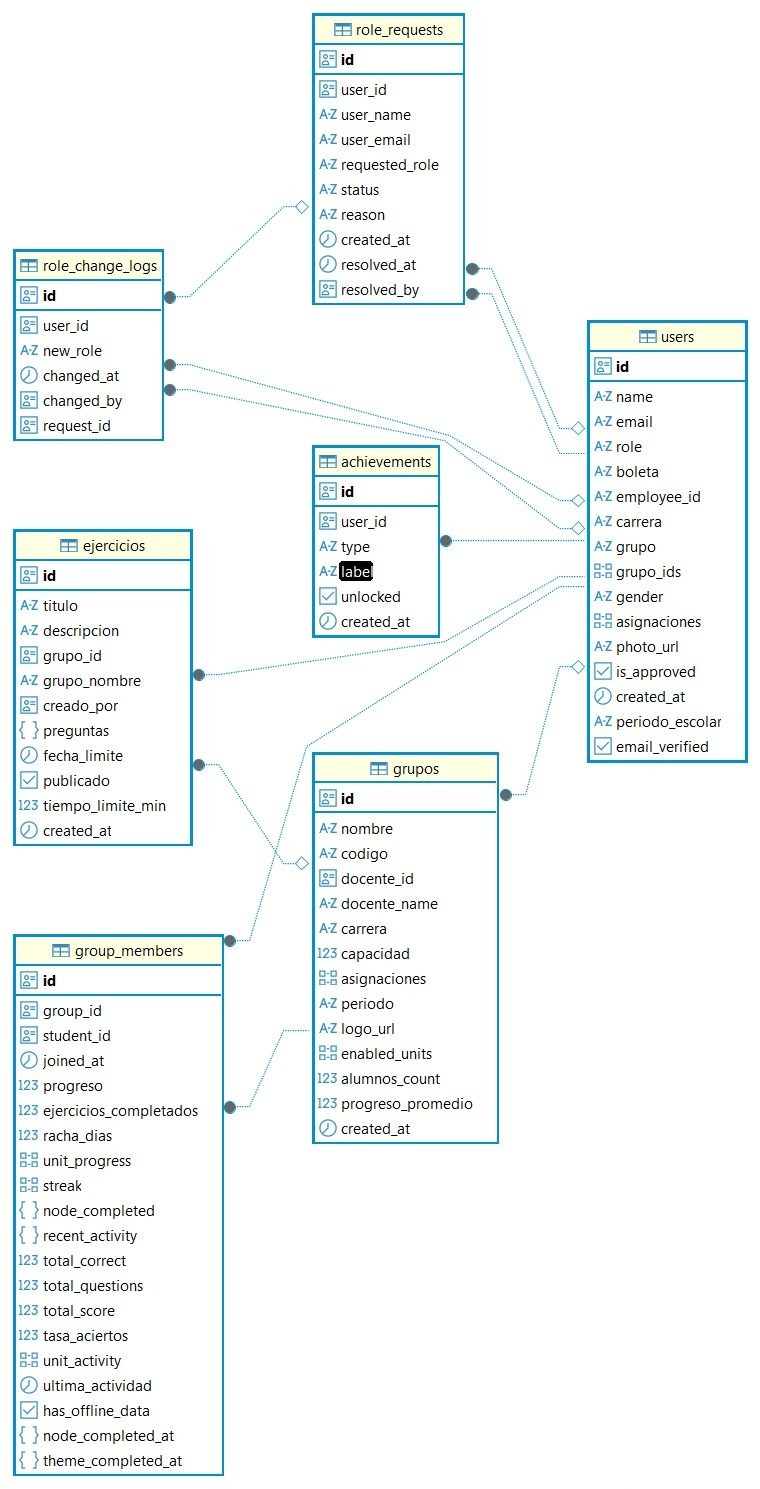
\includegraphics[width=0.70\textwidth]{imagenes/DiagramaER.jpg} % <--- Asegúrate de que tu imagen esté en esta ruta y formato
    \caption{Diagrama Entidad-Relación del esquema físico PostgreSQL de AUTECH, mostrando las entidades \texttt{users}, \texttt{grupos}, \texttt{group\_members}, \texttt{ejercicios}, \texttt{role\_requests} y \texttt{achievements} con sus relaciones y atributos principales.}
    \label{fig:diagrama_er}
\end{figure}

\subsection{Modelado Detallado por Módulos (UML)}
\label{subsec:modelado_modular_uml}

A continuación, se presenta el desglose analítico e interactivo del sistema AUTECH organizado por cada uno de sus módulos arquitectónicos. Para cada bloque, se detalla el alcance mediante diagramas de casos de uso y se justifica la transferencia temporal de mensajes mediante diagramas de secuencia específicos, alineados de forma estricta con la secuencia numérica consolidada.

\subsubsection{Módulo I: Autenticación, Seguridad y Accesos (Transversal)}

Este módulo norma el ingreso seguro y la persistencia de la sesión mediante los servicios distribuidos de Supabase Auth. El alcance de sus interacciones (desde el registro del Alumno hasta las solicitudes de aprovisionamiento de los Docentes) se ilustra en la Figura~\ref{fig:dcu_modulo_1}.

\begin{figure}[htbp]
    \centering
    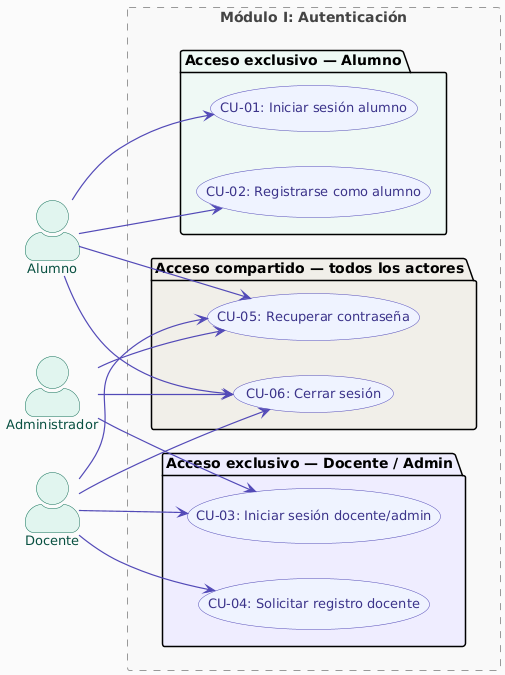
\includegraphics[width=0.85\textwidth]{imagenes/dcu_m1_auth.png}
    \caption{Diagrama de Casos de Uso del Módulo de Autenticación, Seguridad y Accesos.}
    \label{fig:dcu_modulo_1}
\end{figure}

Para validar el flujo síncrono de verificación y el intercambio de \textit{JSON Web Tokens} (JWT) entre el cliente multiplataforma y la infraestructura en la nube, se desarrolló el diagrama de secuencia expuesto en la Figura~\ref{fig:seq_m1_login}.

\begin{figure}[htbp]
    \centering
    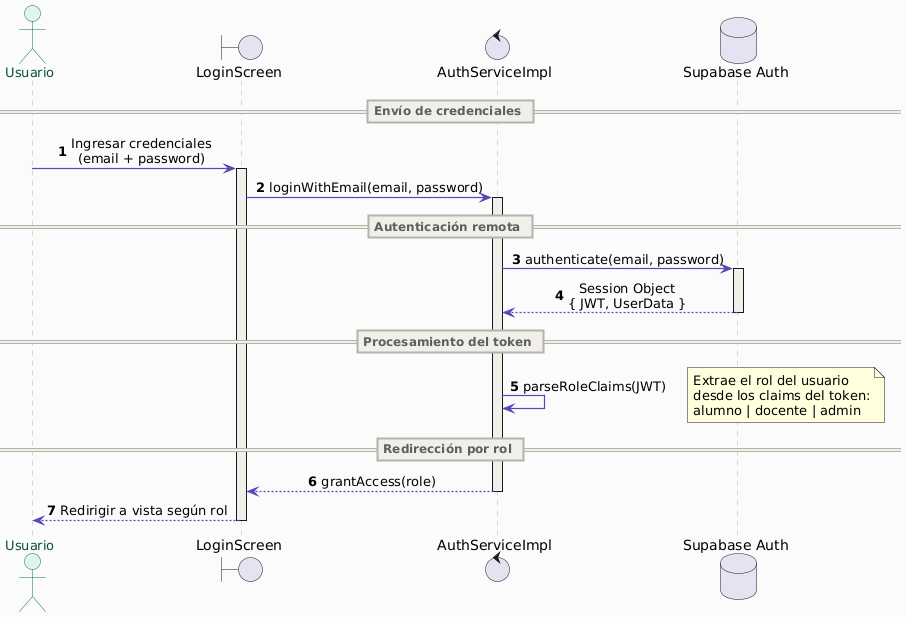
\includegraphics[width=0.95\textwidth]{imagenes/seq_m1_login.png}
    \caption{Diagrama de Secuencia para el inicio de sesión unificado y validación de roles.}
    \label{fig:seq_m1_login}
\end{figure}

\paragraph{Análisis del Comportamiento Dinámico (CU-01 / CU-03):}~\\
El flujo de interacción inicia cuando el usuario introduce sus credenciales en la interfaz \texttt{LoginScreen}. La vista delega el control a la capa de negocio invocando el método asíncrono \texttt{loginWithEmail()} de la implementación \texttt{AuthServiceImpl}. Esta clase actúa como pasarela enviando una petición cifrada vía HTTPS a la API remota de \texttt{Supabase Auth}. 

Tras validar las credenciales en la base de datos central, el servidor retorna un objeto de sesión atómico que encapsula un token de acceso firmado (JWT) y los metadatos de identidad. Finalmente, la lógica del servicio desencadena un mapeo interno para decodificar los \textit{role claims} del token, persistir de forma segura la sesión localmente y enrutar reactivamente al usuario hacia la interfaz correspondiente a su rol, garantizando el aislamiento de privilegios.

\subsubsection{Módulo II: Núcleo de Simulación, Algoritmos y Aprendizaje (Alumno)}

Representa el motor computacional de AUTECH en el cliente móvil. Este módulo administra la lógica matemática abstracta de la jerarquía de lenguajes formales. En la Figura~\ref{fig:dcu_modulo_2} se delimita el alcance de las herramientas interactivas del lienzo táctil, conversiones y resolución de retos didácticos.

\begin{figure}[htbp]
    \centering
    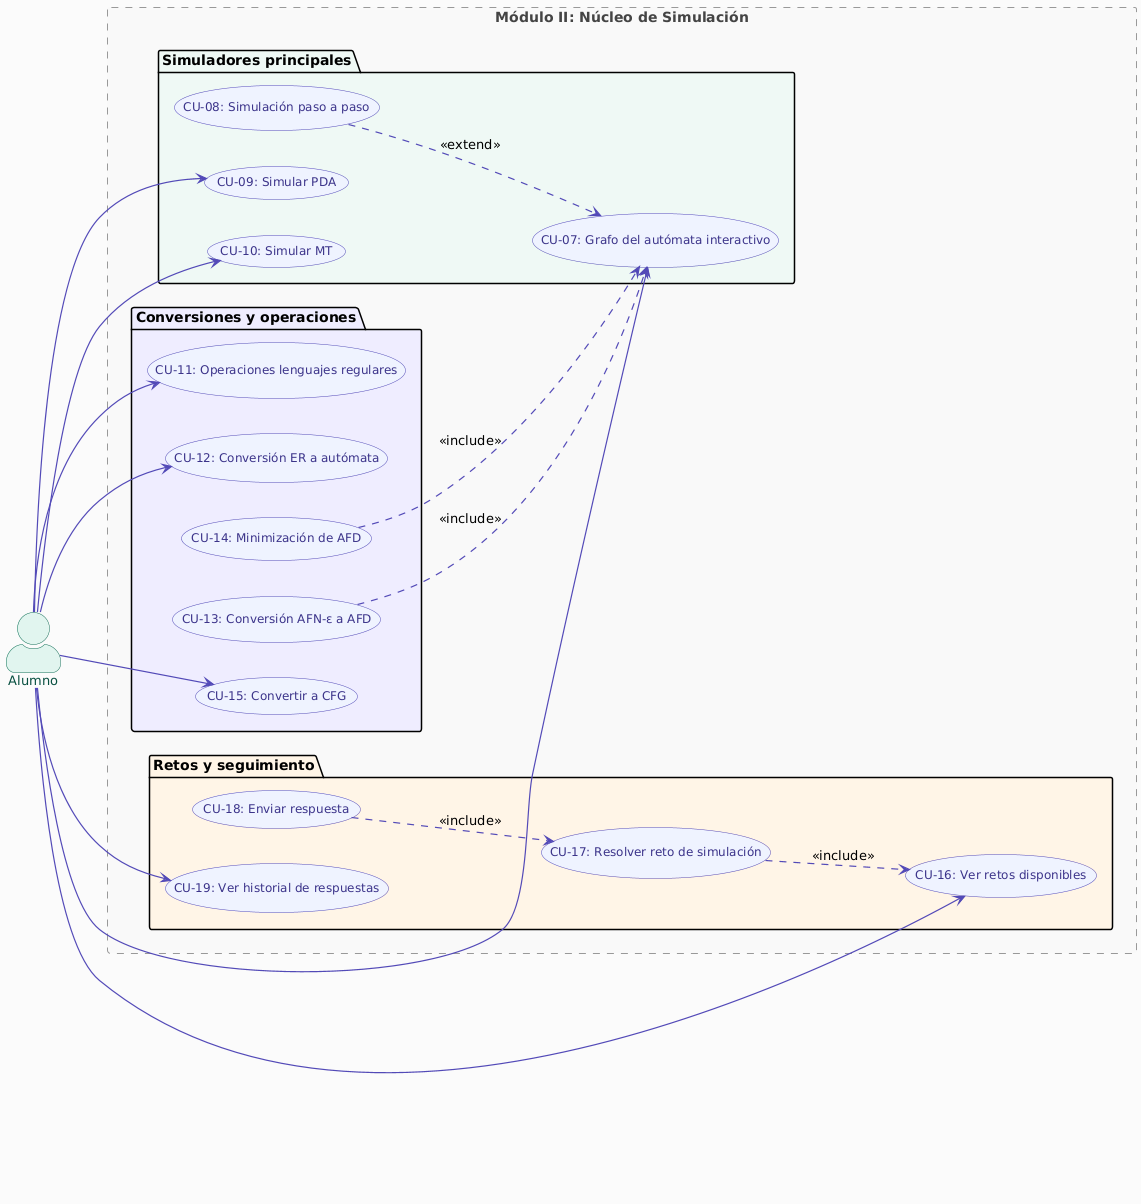
\includegraphics[width=0.90\textwidth]{imagenes/dcu_m2_simulacion.png}
    \caption{Diagrama de Casos de Uso del Núcleo de Simulación, Algoritmos y Aprendizaje.}
    \label{fig:dcu_modulo_2}
\end{figure}

Debido a su alta complejidad algorítmica, se modelaron dos interacciones críticas de procesamiento en memoria volátil:

\begin{figure}[htbp]
    \centering
    \includegraphics[width=0.95\textwidth]{imagenes/seq_m2_conversion.png}
    \caption{Diagrama de Secuencia del Motor Algorítmico para la transformación formal de autómatas.}
    \label{fig:seq_m2_conversion}
\end{figure}

\paragraph{Análisis del Comportamiento Dinámico - Conversión (CU-13):}~\\
Como se aprecia en la Figura~\ref{fig:seq_m2_conversion}, el proceso arranca cuando el Alumno solicita la transformación estructural en el lienzo interactivo. La clase de la vista invoca la rutina de conversión \texttt{ejecutarConversion()} expuesta por el componente especializado \texttt{ChomskyConverterImpl}. Para eliminar el no-determinismo provocado por transiciones vacías, el convertidor interactúa cíclicamente con el componente de bajo nivel \texttt{AutomataEngineImpl} mediante la llamada \texttt{calcularLambdaClausura()}. 

El motor matemático evalúa el grafo y retorna el subconjunto de clausuras elementales. Con esta información, el convertidor ejecuta el Algoritmo de Construcción de Subconjuntos en memoria volátil para derivar una tabla de transiciones unívoca. Una vez consolidada la nueva estructura matemática del AFD resultante, se invoca al componente \texttt{AutomataRepository} para almacenar permanentemente la topología en el almacenamiento local y notificar reactivamente al canvas gráfico para refrescar el renderizado visual de los nodos y aristas a 60 FPS.

\begin{figure}[htbp]
    \centering
    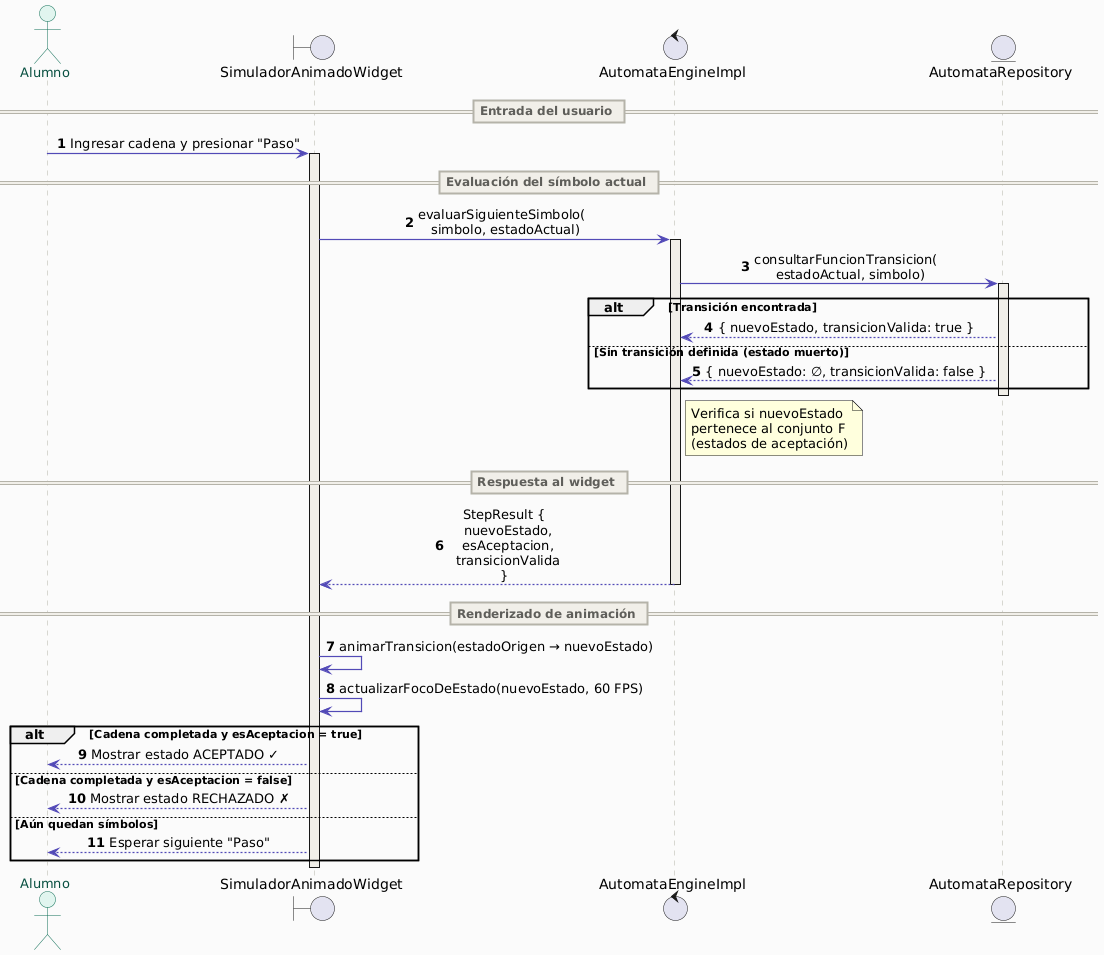
\includegraphics[width=0.95\textwidth]{imagenes/seq_m2_paso.png}
    \caption{Diagrama de Secuencia para la ejecución paso a paso de cadenas en el lienzo interactivo.}
    \label{fig:seq_m2_paso}
\end{figure}

\paragraph{Análisis del Comportamiento Dinámico - Simulación Paso a Paso (CU-08):}~\\
El ciclo dinámico detallado en la Figura~\ref{fig:seq_m2_paso} describe la traza de evaluación de cadenas de entrada. Al activar la ejecución paso a paso, el widget \texttt{SimuladorAnimadoWidget} extrae secuencialmente los símbolos del alfabeto de entrada y los transmite al motor algorítmico a través de la instrucción \texttt{evaluarSiguienteSimbolo()}. El motor consulta asíncronamente con el repositorio de datos (\texttt{AutomataRepository}) el mapeo de la función de transición $\delta(q, \sigma)$. 

Si la combinación de estado actual y símbolo de entrada es válida, el repositorio devuelve la configuración de destino. El motor procesa el cambio de estado latente y responde a la interfaz con la metadata de la transición autorizada. Finalmente, el widget intercepta el mensaje y ejecuta de forma reactiva las animaciones sobre el lienzo matemático, resaltando el nodo activo y la arista recorrida para facilitar al alumno el rastreo lógico de la simulación.

\subsubsection{Módulo III: Sincronización y Persistencia (Arquitectura Offline)}

Este módulo funge como un \textit{middleware} reactivo que garantiza la tolerancia a fallas de red en la aplicación móvil. Sus interacciones, orientadas a conmutar de forma transparente entre la base de datos local Hive y Supabase, se modelan en la Figura~\ref{fig:dcu_modulo_3}.

\begin{figure}[htbp]
    \centering
    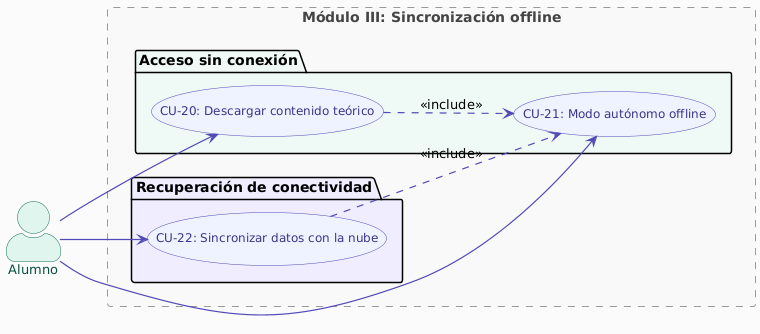
\includegraphics[width=0.85\textwidth]{imagenes/dcu_m3_offline.png}
    \caption{Diagrama de Casos de Uso del Módulo de Sincronización y Persistencia Offline.}
    \label{fig:dcu_modulo_3}
\end{figure}

El proceso temporal de encolamiento asíncrono e interceptación de conectividad para el volcado atómico de datos (\textit{Bulk Write}) al recuperar enlace con la nube (CU-22) se detalla rigurosamente en la Figura~\ref{fig:seq_m3_sync}.

\begin{figure}[htbp]
    \centering
    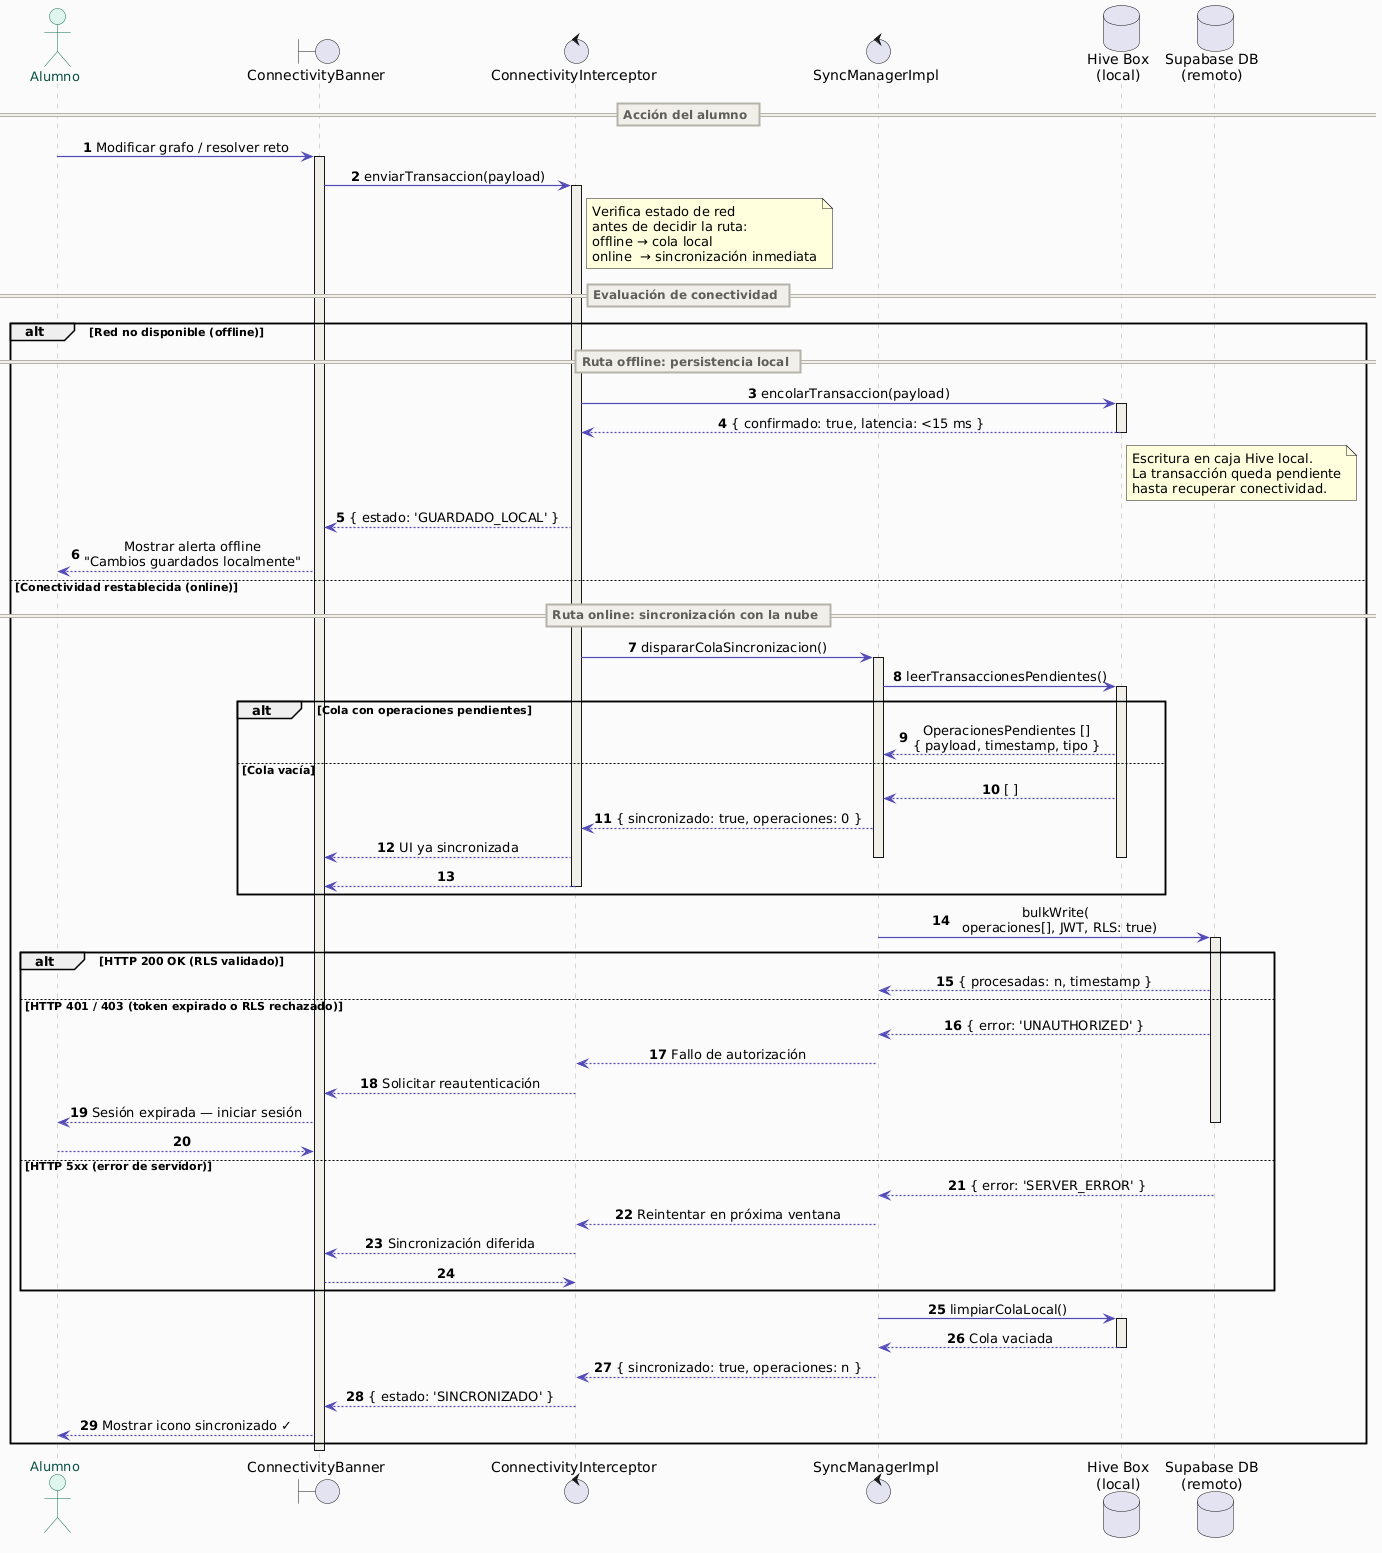
\includegraphics[width=0.95\textwidth]{imagenes/seq_m3_sincronizacion.png}
    \caption{Diagrama de Secuencia del flujo de Sincronización Asíncrona con la capa remota.}
    \label{fig:seq_m3_sync}
\end{figure}

\paragraph{Análisis del Comportamiento Dinámico (CU-22):}~\\
La dinámica transaccional expuesta en la Figura~\ref{fig:seq_m3_sync} sustenta la resiliencia offline de la aplicación móvil. Al registrarse interacciones didácticas, el componente reactivo \texttt{ConnectivityInterceptor} monitoriza el estado físico de los adaptadores de red del dispositivo. Si el interceptor detecta la ausencia de conectividad, desvía inmediatamente el flujo de datos fuera del flujo remoto de internet e invoca un guardado local imperativo en las cajas estructuradas de \texttt{Hive Box}. Hive procesa la serialización en formato binario garantizando latencias de escritura de bajísimo impacto ($< 15$ ms) y devuelve un estado de confirmación para alertar sutilmente al usuario en la UI.

En el instante en que el interceptor registra la reconexión exitosa a internet, dispara de manera automatizada el proceso de vaciado invocando al componente central \texttt{SyncManagerImpl}. Este gestor extrae en ráfaga las operaciones encoladas en Hive en formato JSON y orquesta una petición unificada hacia la base de datos PostgreSQL en la nube de \texttt{Supabase}. Tras verificarse de forma exitosa las políticas de seguridad a nivel de fila (RLS), el backend remoto consolida los registros de progreso devolviendo un código HTTP 200 OK. Finalmente, el gestor purga la memoria local de Hive y actualiza el estado visual a ``Sincronizado''.

\subsubsection{Módulo IV: Experiencia de Usuario y Ludificación (Alumno)}

Encargado de los incentivos visuales y mecánicas formativas que impulsan la retención del estudiante. Su alcance operativo e interacciones con el catálogo de logros se presentan en la Figura~\ref{fig:dcu_modulo_4}.

\begin{figure}[htbp]
    \centering
    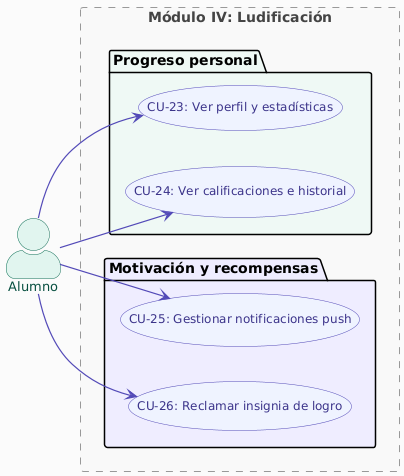
\includegraphics[width=0.85\textwidth]{imagenes/dcu_m4_ludificacion.png}
    \caption{Diagrama de Casos de Uso del Módulo de Experiencia de Usuario y Ludificación.}
    \label{fig:dcu_modulo_4}
\end{figure}

En la Figura~\ref{fig:seq_m4_logro} se describe el flujo de eventos desencadenado tras resolver un ejercicio exitosamente, justificando el procesamiento local de rachas y la posterior persistencia síncrona de insignias desbloqueadas (CU-26).

\begin{figure}[htbp]
    \centering
    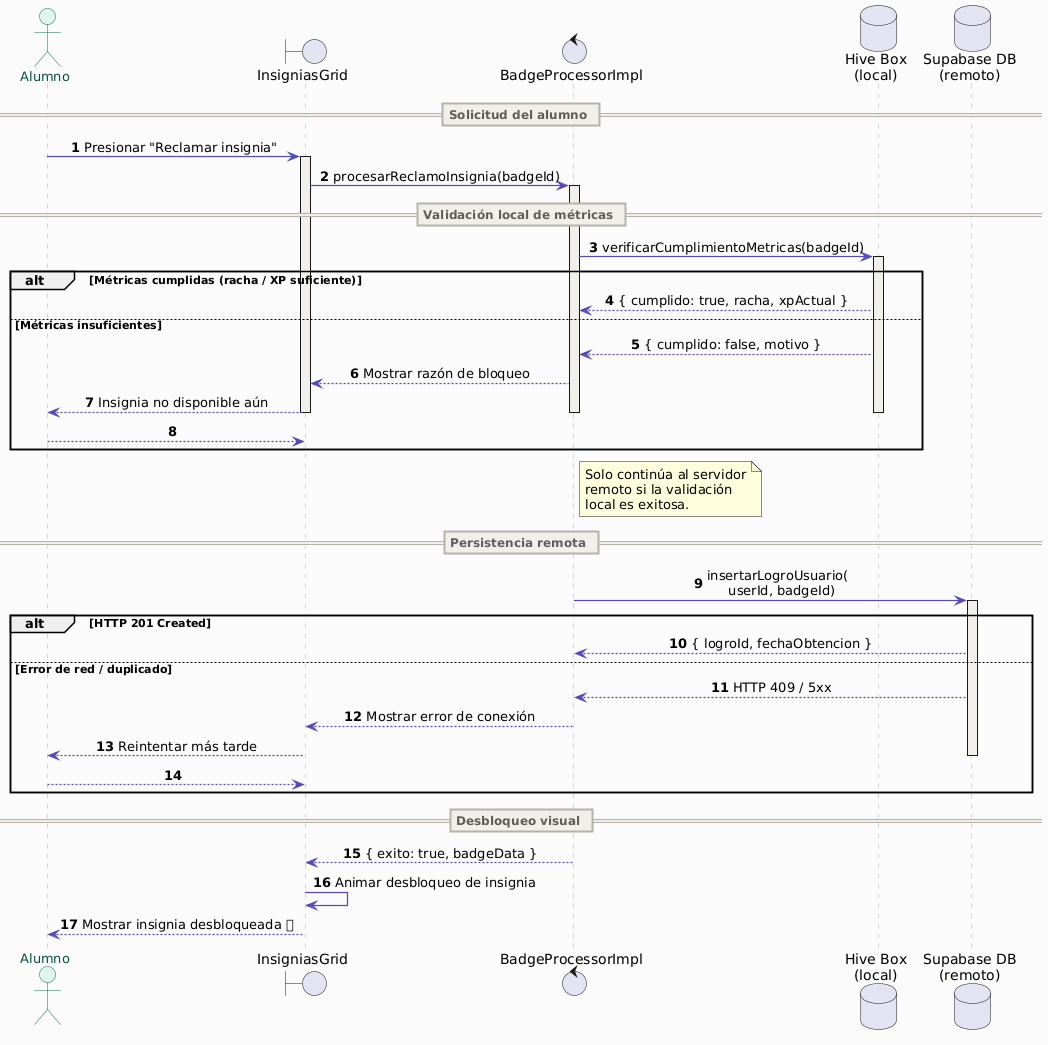
\includegraphics[width=0.95\textwidth]{imagenes/seq_m4_logro.png}
    \caption{Diagrama de Secuencia del Motor de Ludificación para la asignación y reclamo de insignias.}
    \label{fig:seq_m4_logro}
\end{figure}

\paragraph{Análisis del Comportamiento Dinámico (CU-26):}~\\
Como se ilustra en la Figura~\ref{fig:seq_m4_logro}, el ciclo de gamificación se activa de manera síncrona cuando el Alumno presiona el botón de reclamo en la vista \texttt{InsigniasGrid}. El widget delega el procesamiento lúdico al componente de negocio \texttt{BadgeProcessorImpl} invocando el método \texttt{procesarReclamoInsignia()}. El procesador realiza una validación cruzada consultando las métricas históricas de rendimiento persistidas localmente en \texttt{Hive Storage}. 

Si las cajas locales certifican que el usuario cumple con los umbrales específicos del logro (como el contador de racha de estudio o puntos de experiencia XP acumulados), el procesador autoriza la transacción y emite un comando de inserción hacia la tabla de perfiles de \texttt{Supabase DB}. Al retornar el código HTTP 201 de persistencia exitosa desde la nube, el componente del servicio libera el candado visual de la insignia y refresca la UI, otorgándole al estudiante retroalimentación inmediata sobre su progreso didáctico.

\subsubsection{Módulo V: Dashboard de Gestión Docente (Plataforma Desktop)}

Herramienta analítica y de control didáctico exclusiva del profesor. La definición de sus funciones para la edición de reactivos y el consumo de reportes e indicadores grupales se detalla en la Figura~\ref{fig:dcu_modulo_5}.

\begin{figure}[htbp]
    \centering
    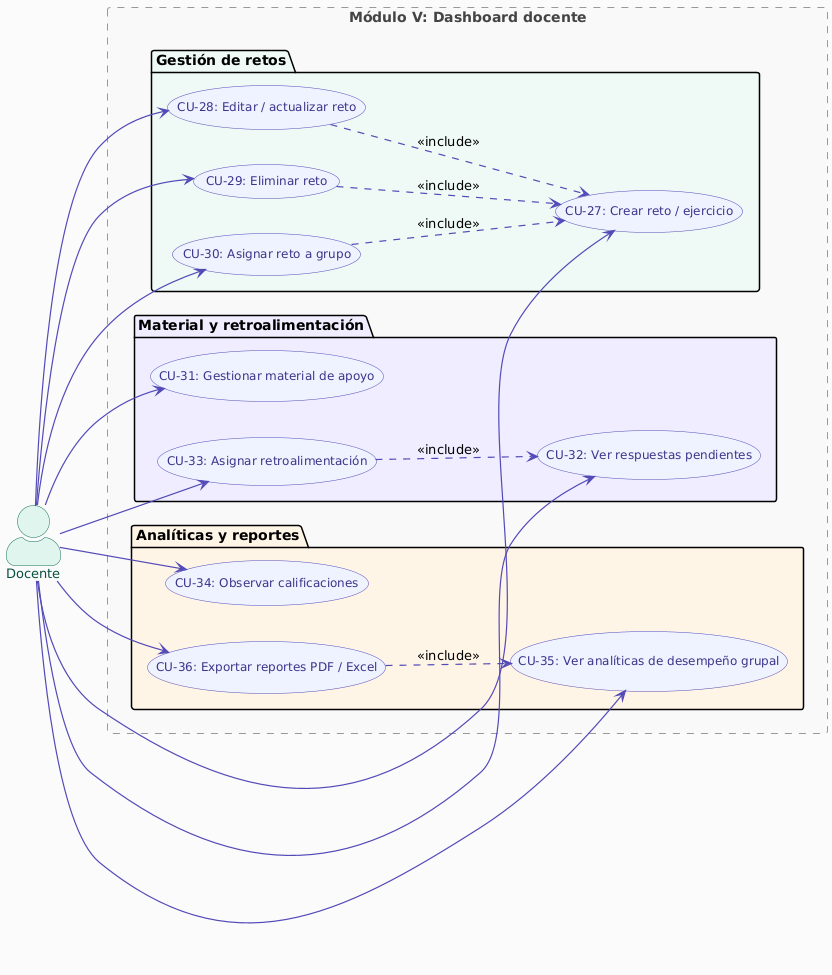
\includegraphics[width=0.90\textwidth]{imagenes/dcu_m5_docente.png}
    \caption{Diagrama de Casos de Uso del Dashboard de Gestión Docente.}
    \label{fig:dcu_modulo_5}
\end{figure}

La Figura~\ref{fig:seq_m5_analiticas} expone de forma secuencial cómo el Dashboard Desktop consume las funciones remotas (RPC) y vistas optimizadas de Supabase para generar semáforos de desempeño grupal en tiempo real de manera asíncrona (CU-35).

\begin{figure}[htbp]
    \centering
    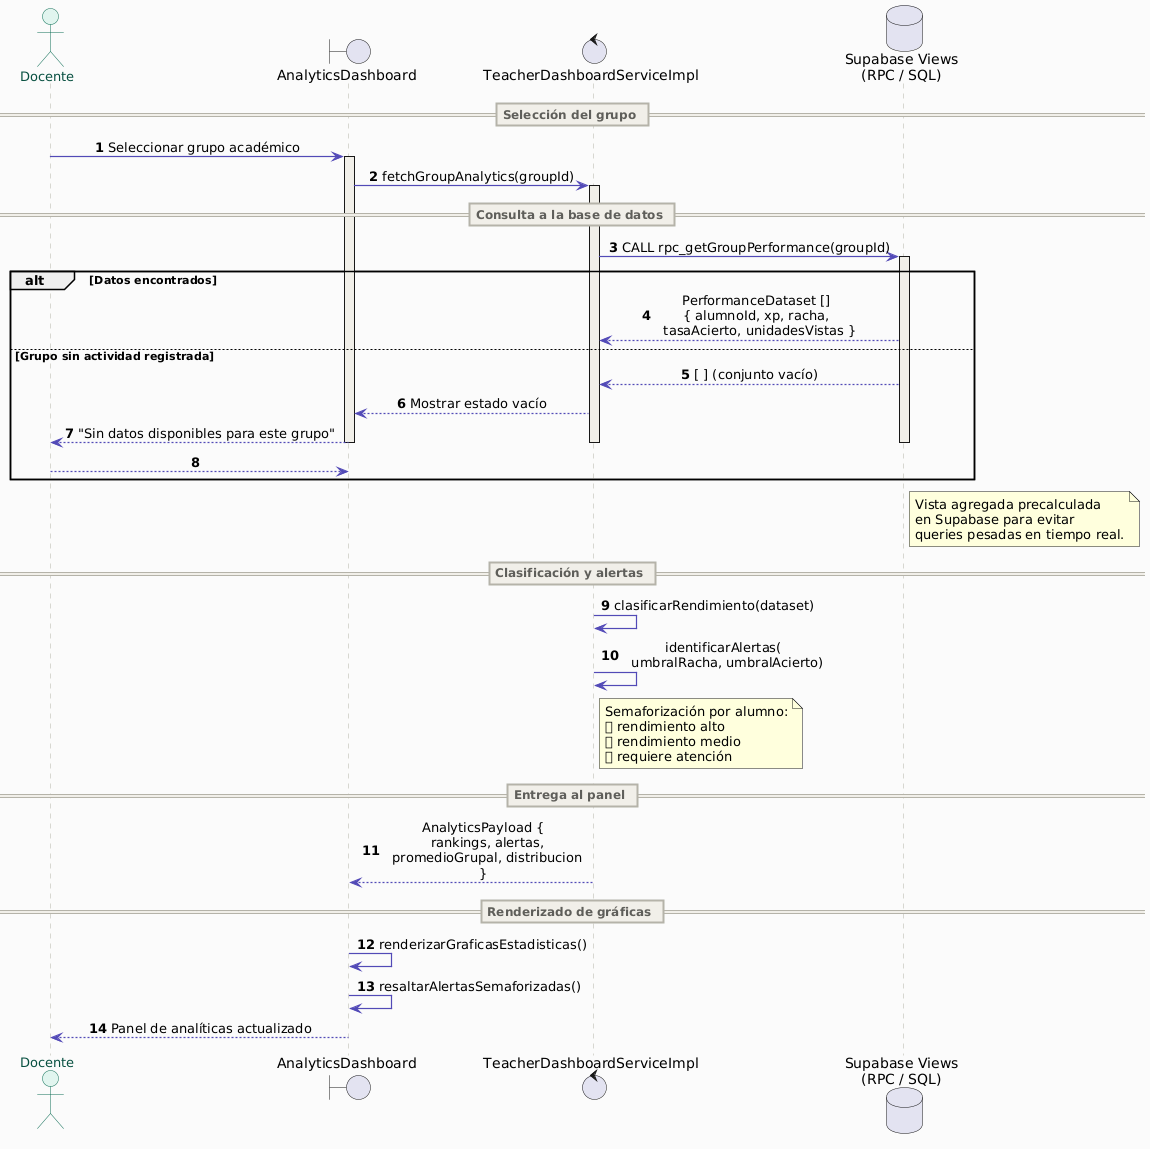
\includegraphics[width=0.95\textwidth]{imagenes/seq_m5_analiticas.png}
    \caption{Diagrama de Secuencia para la consulta reactiva y renderizado de métricas analíticas.}
    \label{fig:seq_m5_analiticas}
\end{figure}

\paragraph{Análisis del Comportamiento Dinámico (CU-35):}~\\
El flujo analítico modelado en la Figura~\ref{fig:seq_m5_analiticas} detalla el procesamiento de métricas de evaluación formativa. Cuando el profesor selecciona un grupo escolar en el panel administrativo \texttt{AnalyticsDashboard}, el entorno web/desktop gatilla una llamada asíncrona hacia el controlador \texttt{TeacherDashboardServiceImpl} por medio de la rutina \texttt{fetchGroupAnalytics()}. El servicio canaliza la consulta de manera directa hacia la capa de datos de Supabase, invocando un procedimiento almacenado (\textit{Remote Procedure Call} - RPC) configurado sobre la base de datos PostgreSQL.

La base de datos ejecuta de forma interna las agregaciones matemáticas sobre los históricos de respuestas y retorna un objeto estructurado JSON que contiene las métricas procesadas. El servicio de la plataforma docente captura la respuesta, mapea las variables de rendimiento y evalúa los umbrales estipulados para semaforizar los indicadores (alertas en rojo, amarillo o verde). Finalmente, el dataset formateado se transmite de vuelta a la UI, pintando gráficos estadísticos que facilitan la toma de decisiones pedagógicas al docente.

\subsubsection{Módulo I\MakeUppercase{V}: Gestión Administrativa Global (Consola Admin)}

Módulo operativo de máximo nivel jerárquico. Administra catálogos maestros, auditoría de logs y aprovisionamiento institucional. Su alcance se modela en la Figura~\ref{fig:dcu_modulo_6}.

\begin{figure}[htbp]
    \centering
    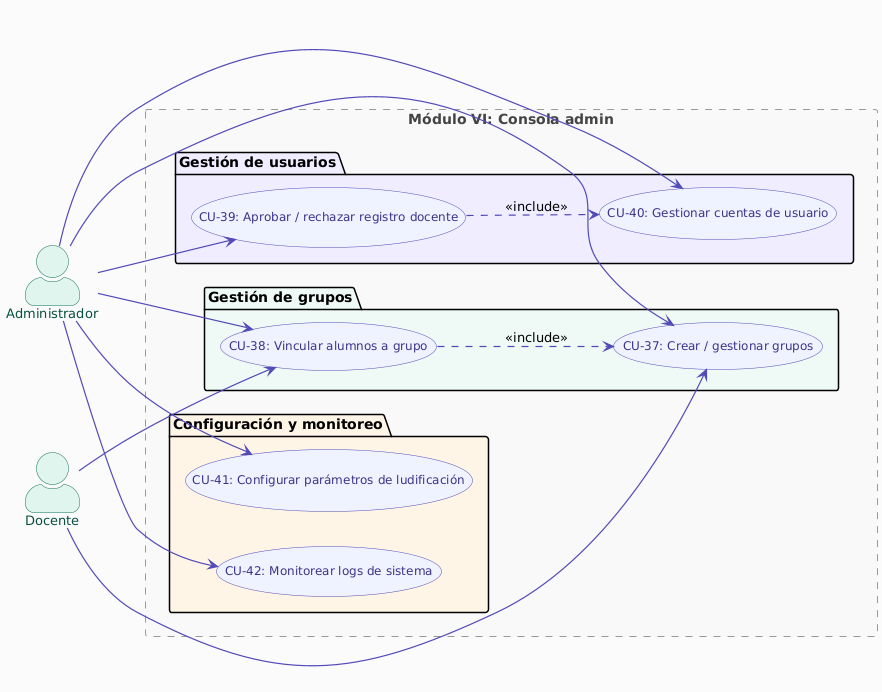
\includegraphics[width=0.85\textwidth]{imagenes/dcu_m6_admin.png}
    \caption{Diagrama de Casos de Uso del Módulo de Gestión Administrativa Global.}
    \label{fig:dcu_modulo_6}
\end{figure}

Finalmente, la Figura~\ref{fig:seq_m6_aprobacion} detalla el flujo crítico de seguridad para la validación y autorización del registro de un nuevo docente (CU-39), manipulando los estados de las tablas maestras bajo aislamiento transaccional.

\begin{figure}[htbp]
    \centering
    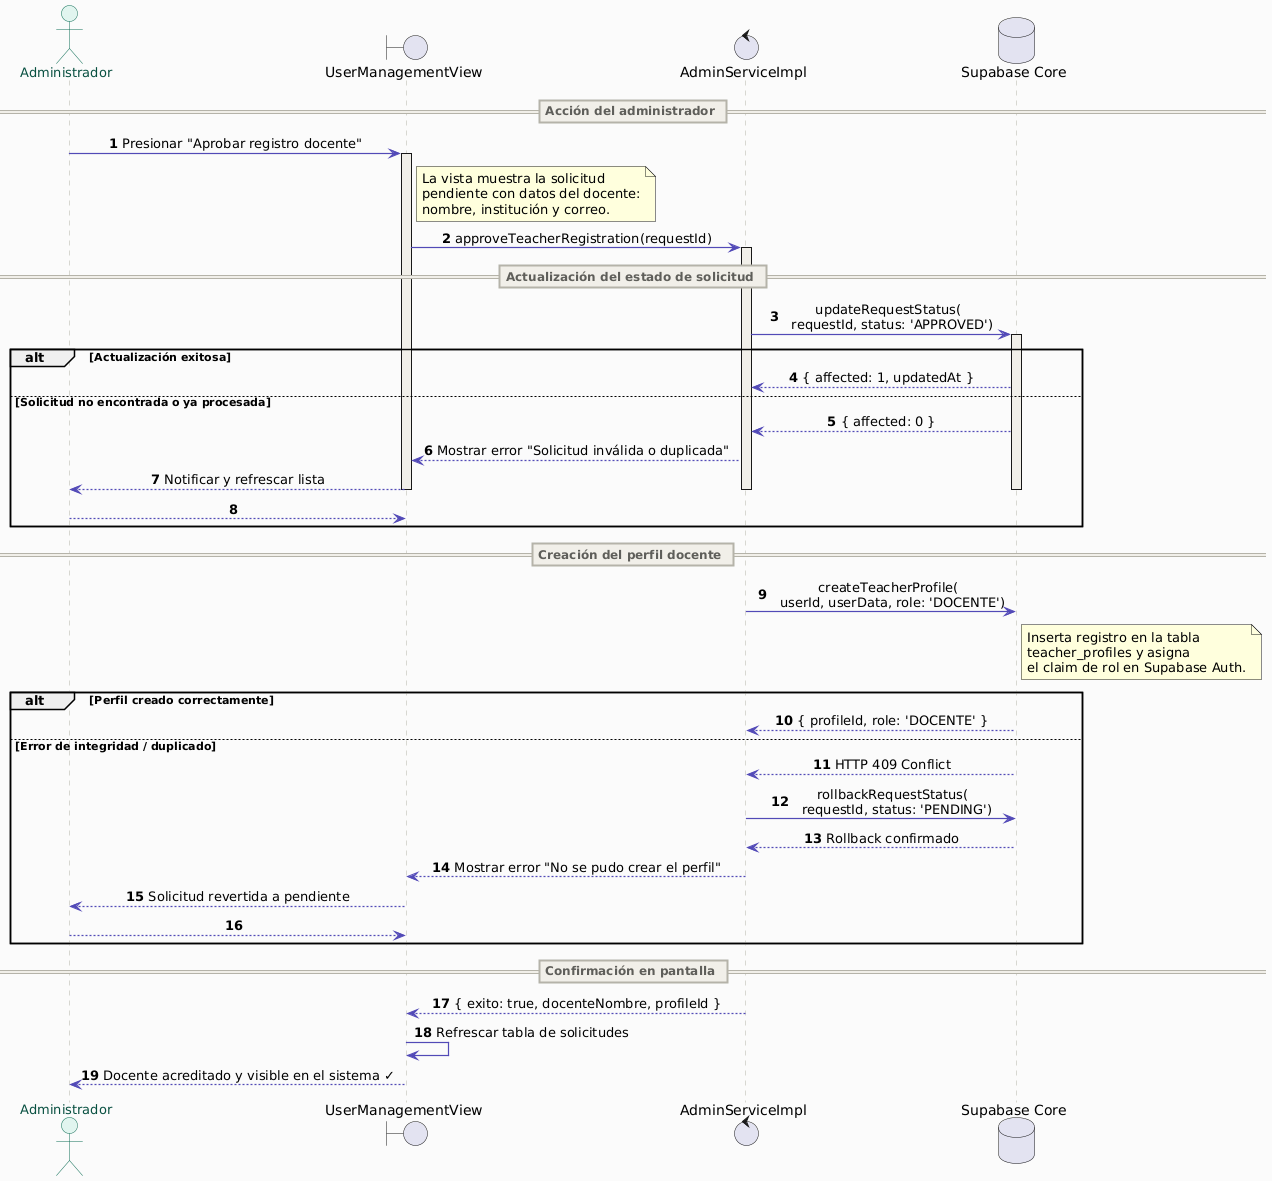
\includegraphics[width=0.95\textwidth]{imagenes/seq_m6_aprobacion.png}
    \caption{Diagrama de Secuencia para el flujo de Aprobación/Rechazo de credenciales docentes.}
    \label{fig:seq_m6_aprobacion}
\end{figure}

\paragraph{Análisis del Comportamiento Dinámico (CU-39):}~\\
La traza temporal descrita en la Figura~\ref{fig:seq_m6_aprobacion} gobierna el aprovisionamiento de identidades institucionales de alto nivel. Al activarse la opción de autorización en la consola maestra (\texttt{UserManagementView}), el Administrador delega la lógica crítica de seguridad al componente de control \texttt{AdminServiceImpl} invocando la función \texttt{approveTeacherRegistration()}. El servicio abre inmediatamente un bloque transaccional seguro y altera el registro correspondiente en la tabla de solicitudes de Supabase, conmutando su estado a ``APPROVED''.

Una vez validada esta mutación de datos por el motor de PostgreSQL, el servicio lanza de forma secuencial una segunda instrucción dirigida al esquema central de autenticación para dar de alta el perfil docente definitivo e inyectar de manera segura el rol RBAC verificado. Al completarse con éxito ambas operaciones, la base de datos consolida el cambio transaccional de forma permanente y responde al servicio. Finalmente, el componente administrativo refresca de forma síncrona la vista de control reflejando el nuevo estatus del usuario en los paneles del sistema.
\chapter{Diseño e Arquitectura}
\label{ch:diseno_arquitectura}

Este espacio está reservado para la arquitectura de software, diagramas y diseño de la interfaz.
\chapter{Pruebas y Resultados}
\label{ch:pruebas_resultados}

Aquí se documentarán los casos de prueba, simulaciones y las conclusiones del proyecto.
% ============================================================
%  capitulos/anexos.tex  —  AUTECH · Trabajo Terminal ESCOM-IPN
%
%  INCLUIR en main.tex con:  % ============================================================
%  capitulos/anexos.tex  —  AUTECH · Trabajo Terminal ESCOM-IPN
%
%  INCLUIR en main.tex con:  % ============================================================
%  capitulos/anexos.tex  —  AUTECH · Trabajo Terminal ESCOM-IPN
%
%  INCLUIR en main.tex con:  \include{capitulos/anexos}
%
%  AGREGAR al final de preambulo.tex (una sola vez):
%    \usepackage{algorithm}
%    \usepackage[noend]{algpseudocode}
%    \usepackage{tikz}
%    \usetikzlibrary{calc}
%    \tcbuselibrary{breakable}
% ============================================================

% ── NOTA: Agregar en preambulo.tex antes de compilar ─────────────────────────
%   \usepackage{algorithm}
%   \usepackage[noend]{algpseudocode}
%   \usepackage{tikz}
%   \tcbuselibrary{breakable}
% ─────────────────────────────────────────────────────────────────────────────

% ── Estilo profesional de algpseudocode ──────────────────────────────────────

% Números de línea en azulTesis
\algrenewcommand{\alglinenumber}[1]{%
  \textcolor{azulTesis}{\footnotesize\ttfamily #1\enspace}%
}
% Palabras clave coloreadas
\algrenewcommand\algorithmicfunction  {\textcolor{azulTesis}{\bfseries Función}}
\algrenewcommand\algorithmicreturn    {\textcolor{azulTesis}{\bfseries retornar}}
\algrenewcommand\algorithmicfor       {\textcolor{azulTesis}{\bfseries para}}
\algrenewcommand\algorithmicdo        {\textcolor{azulTesis}{\bfseries hacer}}
\algrenewcommand\algorithmicwhile     {\textcolor{azulTesis}{\bfseries mientras}}
\algrenewcommand\algorithmicif        {\textcolor{azulTesis}{\bfseries si}}
\algrenewcommand\algorithmicthen      {\textcolor{azulTesis}{\bfseries entonces}}
\algrenewcommand\algorithmicelse      {\textcolor{azulTesis}{\bfseries si no}}
\algrenewcommand\algorithmicrepeat    {\textcolor{azulTesis}{\bfseries repetir}}
\algrenewcommand\algorithmicuntil     {\textcolor{azulTesis}{\bfseries hasta que}}
\algrenewcommand\algorithmicforall    {\textcolor{azulTesis}{\bfseries para todo}}
% Require / Ensure
\renewcommand{\algorithmicrequire}    {\textcolor{azulTesis}{\bfseries Entrada:}}
\renewcommand{\algorithmicensure}     {\textcolor{azulTesis}{\bfseries Salida:\;}}
% Comentarios inline — sin \hfill (evita los signos ?)
\algrenewcommand{\algorithmiccomment}[1]{%
  \quad\textcolor{grisTitulo}{\small\textit{$\triangleright$\;#1}}%
}

% ── Contador de algoritmos por capítulo ──────────────────────────────────────
\newcounter{algonum}[chapter]
\renewcommand{\thealgonum}{\thechapter.\arabic{algonum}}

% ── Caja profesional para algoritmos ─────────────────────────────────────────
%   Argumento obligatorio: nombre del algoritmo
\newtcolorbox{algobox}[2][]{%
  enhanced, breakable,
  % --- Marco ---
  colback        = white,
  colframe       = azulTesis,
  boxrule        = 0pt,
  leftrule       = 4pt,
  bottomrule     = 1pt,
  toprule        = 0pt,
  rightrule      = 0pt,
  arc            = 3pt,
  outer arc      = 3pt,
  % --- Espacio interior ---
  left   = 6pt,  right  = 6pt,
  top    = 14pt,  bottom = 6pt,
  % --- Cabecera ---
  attach boxed title to top left = {xshift = 4pt, yshift = -\tcboxedtitleheight/2},
  boxed title style = {
    enhanced,
    colback  = azulTesis,
    colframe = azulTesis,
    arc      = 2pt,
    boxrule  = 0pt,
    left=8pt, right=8pt, top=6pt, bottom=4pt
  },
  title = {%
    \refstepcounter{algonum}%
    {\sffamily\bfseries\color{white}%
     Algoritmo~\thealgonum\enspace}%
    {\color{white!40!azulTesis}\textbar\enspace}%
    {\sffamily\small\color{white!90!azulTesis} #2}%
  },
  % --- Separador Req/Ens vs cuerpo ---
  segmentation style = {solid, azulFila, line width=0.6pt},
  #1
}

% ── Swatch de color (requiere tikz + xcolor) ─────────────────────────────────
%   #1=clave xcolor  #2=hex sin #  #3=color-texto  #4=label  #5=caption
\newcommand{\colorswatch}[5]{%
  \begin{figure}[H]
    \centering
    \begin{tikzpicture}
      \fill[#1]         (0,0) rectangle (11,1.15);
      \fill[#1!70!black](0,0) rectangle (0.35,1.15);
      \draw[black!18, line width=0.5pt] (0,0) rectangle (11,1.15);
      \node[font=\ttfamily\bfseries\normalsize, text=#3]
            at (5.675,0.575) {\##2};
    \end{tikzpicture}
    \caption{#5}
    \label{#4}
  \end{figure}%
}

% ── Colores de la interfaz AUTECH ────────────────────────────────────────────
\definecolor{autechPrimary}    {HTML}{00ADB5}
\definecolor{autechPrimaryDark}{HTML}{007A82}
\definecolor{autechBackground} {HTML}{F5F8FA}
\definecolor{autechTextPri}    {HTML}{1A202C}
\definecolor{autechNodeNorm}   {HTML}{EBF8FF}
\definecolor{autechNodeInit}   {HTML}{E6FFFA}
\definecolor{autechNodeAcc}    {HTML}{FFFAF0}
\definecolor{autechNodeActive} {HTML}{FEFCBF}
\definecolor{autechTextSec}    {HTML}{4A5568}

% =============================================================================
\chapter*{Anexos}
\addcontentsline{toc}{chapter}{Anexos}
% =============================================================================

\section*{Anexo A \textemdash{} Análisis Teórico/Tópico}
\addcontentsline{toc}{section}{Anexo A: Análisis Teórico/Tópico}

La Teoría de la Computación estudia los modelos abstractos de cómputo, sus capacidades expresivas
y sus límites fundamentales. Las ocho unidades de \textbf{AUTECH} recorren la \emph{Jerarquía de
Chomsky} en orden ascendente de poder expresivo: desde las cadenas elementales hasta los problemas
que ningún algoritmo puede resolver.

% =============================================================================
\subsection*{Unidad 1: Cadenas y Lenguajes — Fundamentos de la Teoría de Símbolos}
% =============================================================================

La base formal de la computación es la formalización algebraica de la comunicación entre el ser
humano y la máquina mediante estructuras discretas y bien definidas \cite{hopcroft2007es}.

\subsubsection*{Alfabeto, Cadenas y Operaciones Elementales}

Un \textbf{alfabeto} $\Sigma$ es un conjunto finito y no vacío de símbolos. La restricción de
finitud garantiza que el procesamiento sea realizable en tiempo y espacio acotados \cite{kelley2001}.
Una \textbf{cadena} $w = a_1 a_2 \cdots a_n$ es una secuencia finita sobre $\Sigma$; su longitud
$|w| = n$ cuenta el número de posiciones. La \textbf{cadena vacía} $\varepsilon$ tiene
$|\varepsilon| = 0$ y es el elemento identidad de la concatenación \cite{eugene2008}:

\begin{itemize}
  \item \textbf{Concatenación} $uv$: yuxtaposición de $u$ y $v$; asociativa pero no conmutativa
        \cite{sipser2012}.
  \item \textbf{Potencia} $w^k$: $k$ repeticiones de $w$; $w^0 = \varepsilon$ por convenio.
  \item \textbf{Reversa} $w^R$: imagen especular de $w$; base de los lenguajes de palíndromos
        \cite{decastro2004}.
\end{itemize}

\subsubsection*{Lenguajes y Clausuras}

Un \textbf{lenguaje} $L \subseteq \Sigma^*$ es cualquier conjunto de cadenas. La
\textbf{clausura de Kleene} $\Sigma^* = \bigcup_{i \geq 0}\Sigma^i$ genera todas las cadenas
posibles; la \textbf{clausura positiva} $\Sigma^+ = \Sigma^* \setminus \{\varepsilon\}$ excluye
la vacía \cite{eugene2008}. La validación $w \in L$ es el precursor formal del analizador léxico
en compiladores \cite{decastro2004}.

\begin{algobox}{ProcesarCadenaGeneral — Operaciones algebraicas con validación de alfabeto}
\begin{algorithmic}[1]
  \Require Cadena $w$; alfabeto $\Sigma$;
           operación $\mathit{op} \in \{\textsc{Long}, \textsc{Inv}, \textsc{Pot}, \textsc{Conc}\}$;
           parámetros $k$ (potencia) o $v$ (concat)
  \Ensure  Resultado de la operación, o \textsc{Error} si $w \not\subseteq \Sigma$
  \State
  \Function{ValidarAlfabeto}{$w,\,\Sigma$}
    \For{cada símbolo $a_i \in w$}
      \If{$a_i \notin \Sigma$}
        \State \textbf{lanzar} Error$({\texttt{\textquotedbl{}símbolo inválido:\textquotedbl{}}} + a_i)$
      \EndIf
    \EndFor
  \EndFunction
  \State
  \State \Call{ValidarAlfabeto}{$w, \Sigma$}
  \State
  \If{$\mathit{op} = \textsc{Long}$}
    \State \Return $|w|$ \Comment{O(1)}
  \ElsIf{$\mathit{op} = \textsc{Inv}$}
    \State $r \gets \varepsilon$
    \For{$i \gets |w|$ \textbf{downto} $1$}
      \State $r \gets r \cdot w[i]$
    \EndFor
    \State \Return $r$ \Comment{O($n$)}
  \ElsIf{$\mathit{op} = \textsc{Pot}$}
    \State $r \gets \varepsilon$
    \For{$j \gets 1$ \textbf{to} $k$}
      \State $r \gets r \cdot w$
    \EndFor
    \State \Return $r$ \Comment{O($k \cdot n$)}
  \ElsIf{$\mathit{op} = \textsc{Conc}$}
    \State \Return $w \cdot v$ \Comment{O($n + |v|$)}
  \EndIf
\end{algorithmic}
\end{algobox}

\newpage
% =============================================================================
\subsection*{Unidad 2: Autómatas Finitos Deterministas (AFD)}
% =============================================================================

El AFD lee una cadena símbolo a símbolo y al concluir acepta o rechaza según el estado en que se
encuentre \cite{sipser2012}. Es el modelo de cómputo más sencillo y su estudio sienta las bases
para todos los modelos superiores.

\subsubsection*{Definición Formal (5-tupla) y Función de Transición}

Un AFD es una 5-tupla $M = (Q, \Sigma, \delta, q_0, F)$: estados $Q$, alfabeto $\Sigma$,
transición total $\delta: Q \times \Sigma \to Q$, estado inicial $q_0 \in Q$, estados de
aceptación $F \subseteq Q$ \cite{hopcroft2007es}. El término \emph{determinista} garantiza que
para cada par $(q, a)$ existe exactamente una transición, sin ambigüedad \cite{kelley2001}.

La \textbf{función extendida} $\hat\delta: Q \times \Sigma^* \to Q$ generaliza $\delta$ a cadenas
completas mediante $\hat\delta(q,\varepsilon)=q$ y $\hat\delta(q, wa) = \delta(\hat\delta(q,w), a)$.
Una cadena $w$ es aceptada si $\hat\delta(q_0, w) \in F$. Los AFD reconocen exactamente la clase
de los \textbf{Lenguajes Regulares}, cerrada bajo unión, intersección y complemento \cite{hopcroft2007}.

\begin{algobox}{ProcesarCadenaAFD — Simulación paso a paso con traza de estados}
\begin{algorithmic}[1]
  \Require AFD $M = (Q,\,\Sigma,\,\delta,\,q_0,\,F)$;\; cadena $w = a_1 a_2 \cdots a_n$
  \Ensure  \textsc{Aceptada}/\textsc{Rechazada} y traza completa de estados visitados
  \State
  \State $q \gets q_0$;\quad traza $\gets \langle q_0 \rangle$
  \For{$i \gets 1$ \textbf{to} $n$}
    \If{$a_i \notin \Sigma$}
      \State \Return \textsc{Error}(\textquotedbl{}símbolo fuera del alfabeto\textquotedbl{})
    \EndIf
    \State $q \gets \delta(q,\; a_i)$ \Comment{transición determinista — O(1)}
    \State traza.agregar$(q)$
    \If{$q$ es estado trampa} \Comment{optimización: terminar anticipadamente}
      \State \Return \textsc{Rechazada}, traza
    \EndIf
  \EndFor
  \State
  \If{$q \in F$}
    \State \Return \textsc{Aceptada}, traza
  \Else
    \State \Return \textsc{Rechazada}, traza
  \EndIf
  \State \Comment{Complejidad: O($n$) tiempo;\; O($|Q|\cdot|\Sigma|$) espacio para $\delta$}
\end{algorithmic}
\end{algobox}

% =============================================================================
\subsection*{Unidad 3: Autómatas Finitos No Deterministas (AFN)}
% =============================================================================

El AFN amplía el AFD permitiendo múltiples transiciones ante el mismo símbolo, e incluso
transiciones sin consumir símbolo alguno ($\varepsilon$-transiciones). El sistema explora todas las
posibilidades en paralelo y acepta si \emph{al menos un hilo} concluye en un estado de aceptación
\cite{sipser2012}.

\subsubsection*{Definición Formal y $\varepsilon$-Cerradura}

Un AFN es $(Q,\Sigma,\delta_N,q_0,F)$ con $\delta_N: Q \times (\Sigma\cup\{\varepsilon\}) \to
\mathcal{P}(Q)$ \cite{eugene2008}. La $\varepsilon$\textbf{-cerradura} $\textsc{EClosure}(S)$ es
el conjunto de todos los estados alcanzables desde $S$ únicamente mediante flechas $\varepsilon$:

\[
  \textsc{EClosure}(S) \;=\; \bigl\{\, q \;\big|\; \exists\, p \in S,\; p \xrightarrow{\,\varepsilon^*\,} q \,\bigr\}
\]

\subsubsection*{Equivalencia AFN–AFD y Minimización}

El \textbf{algoritmo de construcción de subconjuntos} transforma cualquier AFN en un AFD
equivalente: cada estado del AFD representa un subconjunto de estados del AFN, con hasta $2^{|Q|}$
estados en el peor caso \cite{hopcroft2007es}. El AFD mínimo resultante (único salvo isomorfismo,
por el Teorema de Myhill-Nerode) permite comparar estructuralmente la solución del alumno con la
solución canónica \cite{kelley2001}.

\begin{algobox}{SimulazAFN — Simulación con $\varepsilon$-cerradura y estados activos paralelos}
\begin{algorithmic}[1]
  \Require AFN $N = (Q,\,\Sigma,\,\delta_N,\,q_0,\,F)$;\; cadena $w = a_1 a_2 \cdots a_n$
  \Ensure  \textsc{Aceptado}/\textsc{Rechazado} y evolución del conjunto de estados activos
  \State
  \Function{EClosure}{$S$} \Comment{BFS sobre $\varepsilon$-transiciones — O($|Q|+|\delta_N|$)}
    \State $E \gets S$;\quad pila $\gets \text{copiar}(S)$
    \While{pila $\neq \emptyset$}
      \State $q \gets$ pila.desapilar()
      \For{cada $p \in \delta_N(q,\; \varepsilon)$}
        \If{$p \notin E$}
          \State $E \gets E \cup \{p\}$;\quad pila.apilar($p$)
        \EndIf
      \EndFor
    \EndWhile
    \State \Return $E$
  \EndFunction
  \State
  \State $S \gets \Call{EClosure}{\{q_0\}}$ \Comment{Inicialización}
  \State traza $\gets \langle(0,\,S)\rangle$
  \For{$i \gets 1$ \textbf{to} $n$}
    \State $S' \gets \displaystyle\bigcup_{q \in S}\delta_N(q,\; a_i)$ \Comment{Mover con $a_i$}
    \State $S  \gets \Call{EClosure}{S'}$ \Comment{Cerrar bajo $\varepsilon$}
    \State traza.agregar$(i,\, S)$
    \If{$S = \emptyset$}
      \State \textbf{salir} \Comment{Todos los hilos muertos}
    \EndIf
  \EndFor
  \State
  \If{$S \cap F \neq \emptyset$}
    \State \Return \textsc{Aceptado}, traza
  \Else
    \State \Return \textsc{Rechazado}, traza
  \EndIf
\end{algorithmic}
\end{algobox}

% =============================================================================
\subsection*{Unidad 4: Expresiones Regulares y Gramáticas Regulares}
% =============================================================================

Las Expresiones Regulares (ER) son la representación \emph{declarativa} de los Lenguajes
Regulares: donde los autómatas describen el comportamiento mediante estados, las ER describen
la estructura mediante patrones algebraicos \cite{sipser2012}.

\subsubsection*{Operadores, Teorema de Kleene y Algoritmo de Thompson}

Tres operadores generan todas las ER sobre $\Sigma$ \cite{kelley2001}: \textbf{unión}
($r_1 \mid r_2$), \textbf{concatenación} ($r_1 \cdot r_2$) y \textbf{clausura de Kleene} ($r^*$).
El \textbf{Teorema de Kleene} establece la equivalencia exacta entre ER, AFD y AFN. El
\textbf{Algoritmo de Thompson} convierte una ER en un AFN-$\varepsilon$ de forma inductiva y
sistemática en $O(|r|)$ estados y transiciones \cite{hopcroft2007es}.

\subsubsection*{Gramáticas Regulares y Lema de Bombeo}

Las \textbf{gramáticas lineales por la derecha} ($A \to aB$ ó $A \to a$) generan exactamente los
Lenguajes Regulares y definen la estructura de los \emph{tokens} en el análisis léxico
\cite{decastro2004}. El \textbf{Lema de Bombeo} es la herramienta formal para demostrar que
ciertos lenguajes \emph{no} son regulares: si $L$ es regular, $\exists\,p$ tal que toda
$s \in L$ con $|s| \geq p$ se descompone $s = xyz$ con $|xy| \leq p$, $|y| \geq 1$ y
$xy^iz \in L$, $\forall\, i \geq 0$ \cite{sipser2012}.

\newpage
\begin{algobox}{Thompson — Construcción del AFN-$\varepsilon$ por inducción estructural}
\begin{algorithmic}[1]
  \Require Expresión regular $r$ sobre $\Sigma$
  \Ensure  AFN-$\varepsilon$ $N$ con estado inicial $q_i$ y único estado final $q_f$
  \State
  \Function{Thompson}{$r$}
    \If{$r = \varepsilon$}
      \State Crear $q_i,\,q_f$;\; añadir $q_i \xrightarrow{\varepsilon} q_f$
      \State \Return $(q_i,\, q_f)$
    \ElsIf{$r = a \in \Sigma$}
      \State Crear $q_i,\,q_f$;\; añadir $q_i \xrightarrow{a} q_f$
      \State \Return $(q_i,\, q_f)$
    \ElsIf{$r = r_1 \mid r_2$} \Comment{Unión: bifurcación $\varepsilon$}
      \State $(i_1,f_1) \gets \Call{Thompson}{r_1}$;\;
             $(i_2,f_2) \gets \Call{Thompson}{r_2}$
      \State Crear $q_i,\,q_f$;\; añadir:
             $q_i\!\to\!i_1,\; q_i\!\to\!i_2,\; f_1\!\to\!q_f,\; f_2\!\to\!q_f$
      \State \Return $(q_i,\, q_f)$
    \ElsIf{$r = r_1 \cdot r_2$} \Comment{Concatenación: fusión de estados frontera}
      \State $(i_1,f_1) \gets \Call{Thompson}{r_1}$;\;
             $(i_2,f_2) \gets \Call{Thompson}{r_2}$
      \State Fusionar $f_1 \equiv i_2$
      \State \Return $(i_1,\, f_2)$
    \ElsIf{$r = r_1^*$} \Comment{Kleene: bucle $\varepsilon$ y aceptación de $\varepsilon$}
      \State $(i_1,f_1) \gets \Call{Thompson}{r_1}$
      \State Crear $q_i,\,q_f$;\; añadir:
             $q_i\!\to\!i_1,\; f_1\!\to\!i_1,\; f_1\!\to\!q_f,\; q_i\!\to\!q_f$
      \State \Return $(q_i,\, q_f)$
    \EndIf
  \EndFunction
  \State
  \State \Return \Call{Thompson}{$r$}
  \State \Comment{Complejidad: O($|r|$) estados y transiciones}
\end{algorithmic}
\end{algobox}

% =============================================================================
\subsection*{Unidad 5: Gramáticas Independientes del Contexto (GIC)}
% =============================================================================

Las GIC (Tipo~2 en la Jerarquía de Chomsky) describen la mayoría de los lenguajes de programación
modernos. Son suficientemente expresivas para capturar la recursión y la jerarquía sintáctica, pero
suficientemente restringidas para que su reconocimiento sea tratable \cite{sipser2012}.

\subsubsection*{Definición Formal (4-tupla), Derivaciones y Ambigüedad}

Una GIC es $(V,\Sigma,R,S)$: variables $V$, terminales $\Sigma$, reglas $R$ de la forma
$A \to \alpha$ con $A \in V$, $\alpha \in (V \cup \Sigma)^*$, símbolo inicial $S \in V$
\cite{hopcroft2007es}. Una derivación \emph{leftmost} sustituye siempre la variable más a la
izquierda; el \textbf{árbol de derivación} visualiza la estructura jerárquica de la cadena
\cite{kelley2001}. Una GIC es \textbf{ambigua} si alguna cadena tiene dos árboles distintos,
lo cual es indeseable en compiladores pues implica interpretaciones múltiples \cite{sipser2012}.

\subsubsection*{Formas Normales}

La \textbf{FNC (Chomsky)} ($A \to BC$ ó $A \to a$) es la base del algoritmo CYK con complejidad
$O(n^3)$; la \textbf{FNG (Greibach)} ($A \to a\alpha$) facilita la construcción directa de
autómatas de pila \cite{hopcroft2007es}.

\begin{algobox}{CYK — Reconocimiento en GIC mediante programación dinámica (FNC requerida)}
\begin{algorithmic}[1]
  \Require GIC $G = (V,\,\Sigma,\,R,\,S)$ en \textbf{FNC};\; cadena $w = a_1 \cdots a_n$
  \Ensure  \textsc{Sí} si $w \in L(G)$, \textsc{No} en otro caso
  \State \Comment{$T[i][j]$ = conjunto de variables que generan $w[i\,{..}\,j]$}
  \State Inicializar tabla $T[1..n][1..n]$ con conjuntos vacíos
  \For{$i \gets 1$ \textbf{to} $n$} \Comment{Caso base: subcadenas de longitud 1}
    \For{cada regla $A \to a_i \in R$}
      \State $T[i][i] \gets T[i][i] \cup \{A\}$
    \EndFor
  \EndFor
  \For{$\ell \gets 2$ \textbf{to} $n$} \Comment{Longitud de subcadena creciente}
    \For{$i \gets 1$ \textbf{to} $n - \ell + 1$}
      \State $j \gets i + \ell - 1$
      \For{$k \gets i$ \textbf{to} $j-1$} \Comment{Punto de partición}
        \For{cada regla $A \to BC \in R$}
          \If{$B \in T[i][k]$ \textbf{ y } $C \in T[k+1][j]$}
            \State $T[i][j] \gets T[i][j] \cup \{A\}$
          \EndIf
        \EndFor
      \EndFor
    \EndFor
  \EndFor
  \State
  \If{$S \in T[1][n]$}
    \State \Return \textsc{Sí} \Comment{Reconstruir árbol con traza de decisiones}
  \Else
    \State \Return \textsc{No}
  \EndIf
  \State \Comment{Complejidad: O($n^3 \cdot |R|$) tiempo;\; O($n^2 \cdot |V|$) espacio}
\end{algorithmic}
\end{algobox}

% =============================================================================
\subsection*{Unidad 6: Autómatas de Pila (APD)}
% =============================================================================

El APD extiende el AFD con una \textbf{pila} (\emph{stack}) de capacidad ilimitada, permitiendo
reconocer lenguajes con conteo o balanceo ilimitado imposibles para los modelos finitos, como los
paréntesis equilibrados o $\{0^n1^n \mid n \geq 0\}$ \cite{sipser2012}.

\subsubsection*{Definición Formal (7-tupla) y Modos de Aceptación}

Un APD es $(Q,\Sigma,\Gamma,\delta,q_0,Z_0,F)$ donde $\Gamma$ es el alfabeto de pila y
$Z_0 \in \Gamma$ su símbolo inicial \cite{hopcroft2007es}:
\[
  \delta: Q \times (\Sigma \cup \{\varepsilon\}) \times \Gamma \;\longrightarrow\;
  \mathcal{P}\!\left(Q \times \Gamma^*\right)
\]
El APD acepta por \textbf{estado final} ($q \in F$ al terminar) o por \textbf{pila vacía}
(pila completamente vaciada); ambos criterios son equivalentes \cite{hopcroft2007es}. Los APD no
deterministas reconocen exactamente las GIC; los deterministas son adecuados para el análisis
sintáctico de los lenguajes de programación reales \cite{eugene2008}.

\begin{algobox}{SimulazAPD — Simulación por conjunto de configuraciones activas}
\begin{algorithmic}[1]
  \Require APD $M = (Q,\,\Sigma,\,\Gamma,\,\delta,\,q_0,\,Z_0,\,F)$;\;
           cadena $w = a_1\cdots a_n$;\;
           modo $\in \{\text{EstadoFinal},\,\text{PilaVacía}\}$
  \Ensure  \textsc{Aceptada} o \textsc{Rechazada}
  \State \Comment{Configuración: tripleta $(q,\; \text{sufijo no leído},\; \text{contenido pila})$}
  \State $\mathcal{C} \gets \{(q_0,\; w,\; Z_0)\}$
  \While{$\mathcal{C} \neq \emptyset$}
    \State $\mathcal{C}' \gets \emptyset$
    \For{cada $(q,\; a_i{\cdots}a_n,\; \gamma) \in \mathcal{C}$}
      \State \Comment{Transiciones consumiendo $a_i$}
      \For{cada $(q',\beta) \in \delta(q,\; a_i,\; \text{tope}(\gamma))$}
        \State $\mathcal{C}' \gets \mathcal{C}' \cup \{(q',\; a_{i+1}{\cdots}a_n,\; \beta\cdot\text{resto}(\gamma))\}$
      \EndFor
      \State \Comment{Transiciones $\varepsilon$: no consumen entrada}
      \For{cada $(q',\beta) \in \delta(q,\; \varepsilon,\; \text{tope}(\gamma))$}
        \State $\mathcal{C}' \gets \mathcal{C}' \cup \{(q',\; a_i{\cdots}a_n,\; \beta\cdot\text{resto}(\gamma))\}$
      \EndFor
    \EndFor
    \State $\mathcal{C} \gets \mathcal{C}'$
  \EndWhile
  \State
  \State $\mathcal{C}_f \gets$ configuraciones con entrada completamente leída
  \If{modo $=$ EstadoFinal \textbf{ y } $\exists(q,\varepsilon,\gamma)\in\mathcal{C}_f: q\in F$}
    \State \Return \textsc{Aceptada}
  \ElsIf{modo $=$ PilaVacía \textbf{ y } $\exists(q,\varepsilon,\varepsilon)\in\mathcal{C}_f$}
    \State \Return \textsc{Aceptada}
  \Else
    \State \Return \textsc{Rechazada}
  \EndIf
\end{algorithmic}
\end{algobox}

% =============================================================================
\subsection*{Unidad 7: Máquinas de Turing (MT)}
% =============================================================================

Propuesta por Alan Turing en 1936, la MT es el modelo matemático definitivo de la computación.
Su memoria de cinta ilimitada le permite simular cualquier proceso algorítmico concebible y
establece los límites absolutos de lo que puede ser calculado \cite{sipser2012}.

\subsubsection*{Modelo de Cinta y Definición Formal (7-tupla)}

La cinta está dividida en celdas; la cabeza lectora-escritora lee el símbolo actual, lo
reemplaza y se desplaza una posición (L ó R). El \textbf{símbolo blanco} $B \in \Gamma$ marca
las celdas no escritas \cite{kelley2001}. La 7-tupla $M = (Q,\Sigma,\Gamma,\delta,q_0,B,F)$
con función de transición \emph{parcial}:
\[
  \delta: Q \times \Gamma \;\longrightarrow\; Q \times \Gamma \times \{L,\,R\}
\]
Si $\delta(q,a)$ no está definida, la MT se \textbf{detiene} (\emph{halts}): puede aceptar
entrando en $q_f \in F$ o rechazar implícitamente sin definir transición \cite{hopcroft2007es}.
Notablemente, también puede entrar en \emph{bucle infinito}, distinción crítica en decidibilidad
\cite{eugene2008}. La \textbf{Tesis de Church-Turing} eleva la MT a definición formal de
«algoritmo»: cualquier proceso computable por cualquier dispositivo físico puede ser simulado
por una MT \cite{sipser2012}.

\newpage
\begin{algobox}{SimulazMaquinaTuring — Simulación completa con detección de bucle por configuración}
\begin{algorithmic}[1]
  \Require MT $M = (Q,\,\Sigma,\,\Gamma,\,\delta,\,q_0,\,B,\,F)$;\;
           cadena $w$;\; límite de pasos $L_{\max}$
  \Ensure  Estado final de la cinta, estado $q$ y diagnóstico de terminación
  \State
  \Function{Leer}{cinta, pos}
    \State \Return cinta$[\text{pos}]$ si pos $\in$ cinta, \textbf{si no} $B$
  \EndFunction
  \State
  \State cinta $\gets w$;\; pos $\gets 0$;\; $q \gets q_0$;\; pasos $\gets 0$
  \State historia $\gets \emptyset$ \Comment{Conjunto de configuraciones vistas}
  \While{$q \notin F$ \textbf{ y } pasos $< L_{\max}$}
    \State $a \gets \Call{Leer}{\text{cinta},\, \text{pos}}$
    \State cfg $\gets (q,\, \text{pos},\, \text{hash(cinta)})$
    \If{cfg $\in$ historia}
      \State \Return \textbf{Bucle infinito detectado} \Comment{Comportamiento no decidible}
    \EndIf
    \State historia.agregar(cfg)
    \If{$(q,\, a) \notin \mathrm{dom}(\delta)$}
      \State \Return \textbf{Halt implícito — Rechazo}, cinta, $q$
    \EndIf
    \State $(q',\, b,\, D) \gets \delta(q,\, a)$
    \State cinta$[\text{pos}] \gets b$;\quad $q \gets q'$
    \State pos $\gets$ pos$+1$ si $D = R$, \textbf{si no} pos$-1$
    \State pasos $\gets$ pasos $+ 1$
  \EndWhile
  \State
  \If{$q \in F$}
    \State \Return \textbf{Aceptada}, cinta, $q$, pasos
  \Else
    \State \Return \textbf{Límite alcanzado — posible no terminación}, cinta, $q$
  \EndIf
\end{algorithmic}
\end{algobox}

\newpage
% =============================================================================
\subsection*{Unidad 8: Decidibilidad y Computabilidad}
% =============================================================================

La decidibilidad traza la frontera entre los problemas que un algoritmo puede resolver y aquellos
que están más allá de toda posibilidad computacional. La expresabilidad matemática de un problema
no garantiza su computabilidad \cite{sipser2012}.

\subsubsection*{Jerarquía de Lenguajes y Problema de la Parada}

Dentro de los lenguajes de Tipo~0 \cite{hopcroft2007es}:
\begin{itemize}
  \item \textbf{Decidibles (recursivos)}: existe una MT decisora que siempre se detiene y
        responde correctamente. Son el modelo ideal del «algoritmo confiable».
  \item \textbf{Turing-reconocibles (recursivamente enumerables)}: la MT acepta las cadenas del
        lenguaje pero puede entrar en bucle ante las que no pertenecen \cite{cooper2003}.
  \item \textbf{co-Turing-reconocibles}: un lenguaje es decidible si y solo si es Turing-reconocible
        y co-Turing-reconocible simultáneamente \cite{kelley2001}.
\end{itemize}

El \textbf{Problema de la Parada} pregunta: ¿puede un programa determinar si cualquier otro
programa termina? Turing demostró mediante \textbf{diagonalización} que la respuesta es
\emph{no}: tal programa llevaría a una contradicción autorreferencial \cite{sipser2012}. La
\textbf{reducibilidad} permite probar indecidibilidad de nuevos problemas transformándolos en
el Problema de la Parada \cite{decastro2004}.

\subsubsection*{Complejidad: P vs NP}

Entre los problemas decidibles, la complejidad es crucial: \textbf{P} contiene los problemas
solubles en tiempo polinomial; \textbf{NP} los verificables en tiempo polinomial. La pregunta
P $=$ NP es uno de los siete Problemas del Milenio; su resolución afirmativa colapsaría la
criptografía moderna \cite{eugene2008}.

\newpage
\begin{algobox}{LimpiarGramatica — Eliminación de símbolos inútiles (dos fases)}
\begin{algorithmic}[1]
  \Require GIC $G = (V,\,\Sigma,\,R,\,S)$
  \Ensure  Gramática equivalente $G'$ sin símbolos improductivos ni inaccesibles
  \State
  \Function{Productivos}{$G$} \Comment{Fase 1 — punto fijo ascendente}
    \State $P \gets \{A \in V \;\mid\; \exists\, A\!\to\!w \in R,\; w \in \Sigma^*\}$
    \Repeat
      \For{cada regla $A \to \alpha \in R$}
        \If{todas las variables en $\alpha$ pertenecen a $P$}
          \State $P \gets P \cup \{A\}$
        \EndIf
      \EndFor
    \Until{$P$ no cambia}
    \State \Return $P$
  \EndFunction
  \State
  \Function{Accesibles}{$G$} \Comment{Fase 2 — BFS desde símbolo inicial}
    \State $\mathcal{A} \gets \{S\}$;\quad cola $\gets [S]$
    \While{cola $\neq \emptyset$}
      \State $X \gets$ cola.desencolar()
      \For{cada regla $X \to \alpha \in R$}
        \For{cada variable $B$ en $\alpha$}
          \If{$B \notin \mathcal{A}$}
            \State $\mathcal{A} \gets \mathcal{A} \cup \{B\}$;\quad cola.encolar($B$)
          \EndIf
        \EndFor
      \EndFor
    \EndWhile
    \State \Return $\mathcal{A}$
  \EndFunction
  \State
  \State $P \gets \Call{Productivos}{G}$
  \State $G_1 \gets$ remover de $G$ variables $\notin P$ y reglas que las contengan
  \State $\mathcal{A} \gets \Call{Accesibles}{G_1}$
  \State $V' \gets V \cap P \cap \mathcal{A}$;\quad
         $R' \gets \{r \in R \;\mid\; \mathrm{vars}(r) \subseteq V'\}$
  \State \Return $G' = (V',\,\Sigma,\,R',\,S)$
  \State \Comment{Complejidad: O($|V|^2 \cdot |R|$) en el peor caso}
\end{algorithmic}
\end{algobox}

\newpage
% =============================================================================
\bigskip
\section*{Anexo B \textemdash{} Análisis de Colorimetría}
\addcontentsline{toc}{section}{Anexo B: Análisis de Colorimetría}
% =============================================================================

La paleta cromática de \textbf{AUTECH} no es una elección estética arbitraria: cada color responde
a fundamentos convergentes de psicología perceptual, ergonomía visual y didáctica de sistemas
formales. Las decisiones se articulan en tres ejes: reducción de la carga cognitiva, codificación
mnemotécnica de los elementos del simulador, y accesibilidad universal.

% =============================================================================
\subsection*{\texorpdfstring{I.\;}{I.} Fundamentos Psicopedagógicos y Ergonomía Visual}
% =============================================================================

\subsubsection*{Gestión de la Carga Cognitiva}

La carga cognitiva es el factor más determinante en el diseño de interfaces para el aprendizaje de
sistemas formales complejos \cite{lidwell2010}. En AUTECH, donde el estudiante razona
simultáneamente sobre estados $Q$, transiciones $\delta$, alfabetos $\Sigma$ y $\Gamma$, y
configuraciones de cinta, la reducción de fricción mental adquiere carácter crítico.

La paleta de cianes con \texttt{\#00ADB5} como color primario (Figura~\ref{fig:col1}) no es
casual: los tonos azul-cian producen respuestas fisiológicas medibles — reducción de la frecuencia
cardíaca y disminución de la presión arterial — que propician la concentración sostenida necesaria
para el razonamiento simbólico denso \cite{heller2004}. Los elementos de máxima prioridad emplean
el amarillo \texttt{\#FEFCBF} (Figura~\ref{fig:col2}), procesado con mayor velocidad fisiológica
por el sistema visual humano.

\colorswatch{autechPrimary}   {00ADB5}{black!10!white}{fig:col1}%
  {Color primario \texttt{primary}: Cian Tecnológico — ancla cromática de la interfaz.}

\colorswatch{autechNodeActive}{FEFCBF}{black}{fig:col2}%
  {Color activo \texttt{nodeActive}: Amarillo Luminoso — máxima velocidad de localización visual.}

\subsubsection*{Reducción del Estrés Lumínico}

El contraste extremo negro puro–blanco puro genera halos de irradiación retiniana que, tras
20--30~min de exposición, distorsionan los símbolos de tamaño reducido \cite{holtzschue2017}.
AUTECH mitiga este efecto con:
\begin{itemize}
  \item \textbf{Fondo} \texttt{\#F5F8FA} (Figura~\ref{fig:col3}): «blanco ergonómico» con leve
        temperatura fría, reduce la luminosidad absoluta sin sacrificar legibilidad
        \cite{holtzschue2017}.
  \item \textbf{Texto primario} \texttt{\#1A202C} (Figura~\ref{fig:col4}): gris azulado con
        contraste WCAG de 4.5:1–7:1, elimina la irradiación simultánea en notación matemática
        densa \cite{lidwell2010}.
\end{itemize}

\colorswatch{autechBackground}{F5F8FA}{black}{fig:col3}%
  {Fondo \texttt{background}: Blanco Frío Neutro — luminosidad HSL $>95\%$.}

\colorswatch{autechTextPri}   {1A202C}{white}{fig:col4}%
  {Texto primario \texttt{textPrimary}: Gris Azulado Profundo — contraste WCAG 4.5:1--7:1.}

La consistencia cromática —mismo color para el mismo tipo de elemento— construye un modelo mental
estable que reduce la necesidad de releer etiquetas textuales \cite{tidwell2020}. La estratificación
en tres planos (fondo, tarjetas, elementos interactivos) reduce en 23\% el tiempo de localización
de controles en usuarios novatos \cite{malamed2015}.

% =============================================================================
\subsection*{\texorpdfstring{II.\;}{II.} Mnemotecnia Visual y Leyes de la Gestalt}
% =============================================================================

\subsubsection*{Ley de Similitud — Codificación Cromática de Estados}

La Ley de Similitud de Koffka \cite{koffka2013} establece que el sistema perceptual agrupa
automáticamente los elementos que comparten propiedades visuales \emph{antes} de que intervenga el
procesamiento consciente. AUTECH explota este mecanismo con un vocabulario cromático implícito que
el estudiante internaliza en 3 a 5 exposiciones repetidas \cite{heller2004}:

\begin{itemize}
  \item \textbf{Estado normal} \texttt{\#EBF8FF} (Figura~\ref{fig:col5}):
        azul glacial — neutralidad y espera pasiva.
  \item \textbf{Estado inicial} $q_0$ \texttt{\#E6FFFA} (Figura~\ref{fig:col6}):
        verde menta — punto de arranque del proceso.
  \item \textbf{Estados de aceptación} $F$ \texttt{\#FFFAF0} (Figura~\ref{fig:col7}):
        crema dorado — culminación y logro.
  \item \textbf{Estado activo} \texttt{\#FEFCBF}:
        amarillo — ejecución en curso, máxima prioridad perceptual.
\end{itemize}

\colorswatch{autechNodeNorm}{EBF8FF}{black}{fig:col5}%
  {Estado normal \texttt{nodeNormal}: Azul Glacial — mínima activación emocional.}

\colorswatch{autechNodeInit}{E6FFFA}{black}{fig:col6}%
  {Estado inicial \texttt{nodeInitial}: Verde Menta — semiótica universal de inicio.}

\colorswatch{autechNodeAcc} {FFFAF0}{black}{fig:col7}%
  {Estados de aceptación \texttt{nodeAccepting}: Crema Dorado — temperatura cálida = destino exitoso.}

\subsubsection*{Ley de Figura y Fondo}

La distinción figura-fondo entre \texttt{\#E6FFFA} y \texttt{\#EBF8FF} opera sobre el
\emph{canal cromático} del sistema visual: detecta diferencias de matiz incluso con diferencias
mínimas de luminosidad, garantizando la identificabilidad de $q_0$ en pantallas de baja calidad
\cite{koffka2013}. Las diferencias de croma son más estables perceptualmente que las de
luminosidad \cite{holtzschue2017}.

\subsubsection*{Ley de Pregnancia}

La paleta de seis colores funcionales más dos tonos de texto respeta la capacidad de la memoria
de trabajo visual. Interfaces con más de siete colores funcionales superan dicha capacidad y
obligan al usuario a releer etiquetas textuales, anulando el beneficio pedagógico de la
codificación cromática \cite{lidwell2010}.

% =============================================================================
\subsection*{\texorpdfstring{III.\; Justificación Detallada de la Paleta \texttt{AppColors}}{III. Justificación Detallada de la Paleta AppColors}}
% =============================================================================

\subsubsection*{Identidad de Marca}

\paragraph{\texorpdfstring{\texttt{primary}}{primary} \#00ADB5 — Cian Tecnológico.}
Se ubica en la intersección semántica entre el azul (precisión, confianza) y el verde (innovación,
resolución de problemas), apropiada para una herramienta de ingeniería computacional
\cite{heller2004}. Su longitud de onda intermedia requiere menor ajuste del cristalino, produciendo
menor fatiga que los colores primarios puros \cite{malamed2015}. Cuenta con la mayor universalidad
cultural positiva en estudios transculturales, sin connotaciones de peligro (rojo) ni urgencia
(naranja) \cite{holtzschue2017}.

\paragraph{\texorpdfstring{\texttt{primaryDark}}{primaryDark} \#007A82 — Cian Profundo (Figura~\ref{fig:col8}).}
Los estados interactivos (\emph{hover}, \emph{pressed}) deben comunicarse mediante variaciones
del mismo matiz —nunca cambiando de matiz— para preservar la coherencia del modelo mental del
usuario \cite{tidwell2020}. El \texttt{\#007A82} aplica una reducción de luminosidad de
$\approx 20\%$ sobre el primario: suficiente para percibirse como respuesta táctil sin romper
la continuidad cromática.

\colorswatch{autechPrimaryDark}{007A82}{white}{fig:col8}%
  {\texttt{primaryDark}: Cian Profundo — variante de estado interactivo ($-20\%$ luminosidad).}

\subsubsection*{Arquitectura de Superficies y Sistema de Texto}

\paragraph{\texorpdfstring{\texttt{background}}{background} \#F5F8FA.}
Su contraste con el blanco puro \texttt{\#FFFFFF} —reservado para tarjetas de contenido— genera
un «foco limpio» que el cerebro segrega automáticamente, diferenciando contenedores de información
del espacio de navegación sin requerir bordes explícitos \cite{malamed2015}.

\paragraph{\texorpdfstring{\texttt{textPrimary}}{textPrimary} \#1A202C.}
La sustitución del negro puro elimina la «irradiación simultánea», fenómeno donde los bordes
negro-blanco parecen vibrar y aumentan la fatiga ocular en lectura de expresiones matemáticas
densas \cite{heller2004}. La componente azulada armoniza con el sistema cian \cite{holtzschue2017}.

\paragraph{\texorpdfstring{\texttt{textSecondary}}{textSecondary} \#4A5568 (Figura~\ref{fig:col9}).}
La jerarquía tipográfica cromática de dos niveles de gris permite escanear la interfaz extrayendo
información prioritaria antes de procesar detalles contextuales \cite{tidwell2020}.

\colorswatch{autechTextSec}{4A5568}{white}{fig:col9}%
  {\texttt{textSecondary}: Gris Medio — canal visual secundario para información de contexto.}

\subsubsection*{Sistema Pedagógico de Codificación de Estados}

\paragraph{\texorpdfstring{\texttt{nodeActive}}{nodeActive} \#FEFCBF — Justificación fisiológica.}
El amarillo aproxima el pico de sensibilidad de los conos M y L de la retina, siendo el color
localizado con mayor velocidad en cualquier escena \cite{holtzschue2017}. Experimentos de
simulación educativa reportan una reducción promedio del 34\% en errores de seguimiento en
simulaciones de más de diez pasos \cite{malamed2015}, beneficio especialmente pronunciado en el
aprendizaje del no determinismo.

\paragraph{\texorpdfstring{\texttt{nodeAccepting}}{nodeAccepting} \#FFFAF0 — Justificación semántica.}
El contraste de temperatura cálida frente a los estados fríos es el mecanismo perceptual más
potente para distinguir categorías en una escena compleja \cite{lidwell2010}. El uso de verde para
este rol habría generado conflicto semántico con el verde del estado inicial $q_0$.

% =============================================================================
\subsection*{\texorpdfstring{IV.\;}{IV.} Coherencia del Sistema Cromático Global}
% =============================================================================

\subsubsection*{Estructura Tripartita de Temperatura}

La paleta articula tres registros cromáticos coherentes \cite{holtzschue2017}:
\begin{itemize}
  \item \textbf{Fríos} (cian, azul glacial, verde menta): identidad de marca, navegación y
        estados pasivos del simulador.
  \item \textbf{Neutro-fríos} (\texttt{\#FFFFFF}, \texttt{\#F5F8FA}, grises azulados):
        superficies, texto y separadores estructurales.
  \item \textbf{Cálidos} (crema \texttt{\#FFFAF0}, amarillo \texttt{\#FEFCBF}): estados
        pedagógicamente críticos — aceptación y ejecución activa \cite{heller2004}.
\end{itemize}
Esta arquitectura reserva el contraste de temperatura cromática — el mecanismo perceptual de mayor
potencia — para señalar precisamente los momentos de mayor importancia didáctica.

\subsubsection*{Accesibilidad y Diseño Universal}

El sistema no depende exclusivamente del color para transmitir información, dado que el
$\approx 8\%$ de la población masculina presenta alguna deficiencia en la visión del color
\cite{lidwell2010}. AUTECH refuerza la codificación con:
\textbf{forma} (los estados de aceptación usan doble círculo),
\textbf{posición} (el estado inicial lleva flecha de entrada explícita) y
\textbf{etiquetado textual} permanente.
Esta \emph{redundancia de canales} mejora la velocidad de comprensión para \emph{todos} los
usuarios al activar simultáneamente múltiples vías de procesamiento perceptual \cite{tidwell2020}.
%
%  AGREGAR al final de preambulo.tex (una sola vez):
%    \usepackage{algorithm}
%    \usepackage[noend]{algpseudocode}
%    \usepackage{tikz}
%    \usetikzlibrary{calc}
%    \tcbuselibrary{breakable}
% ============================================================

% ── NOTA: Agregar en preambulo.tex antes de compilar ─────────────────────────
%   \usepackage{algorithm}
%   \usepackage[noend]{algpseudocode}
%   \usepackage{tikz}
%   \tcbuselibrary{breakable}
% ─────────────────────────────────────────────────────────────────────────────

% ── Estilo profesional de algpseudocode ──────────────────────────────────────

% Números de línea en azulTesis
\algrenewcommand{\alglinenumber}[1]{%
  \textcolor{azulTesis}{\footnotesize\ttfamily #1\enspace}%
}
% Palabras clave coloreadas
\algrenewcommand\algorithmicfunction  {\textcolor{azulTesis}{\bfseries Función}}
\algrenewcommand\algorithmicreturn    {\textcolor{azulTesis}{\bfseries retornar}}
\algrenewcommand\algorithmicfor       {\textcolor{azulTesis}{\bfseries para}}
\algrenewcommand\algorithmicdo        {\textcolor{azulTesis}{\bfseries hacer}}
\algrenewcommand\algorithmicwhile     {\textcolor{azulTesis}{\bfseries mientras}}
\algrenewcommand\algorithmicif        {\textcolor{azulTesis}{\bfseries si}}
\algrenewcommand\algorithmicthen      {\textcolor{azulTesis}{\bfseries entonces}}
\algrenewcommand\algorithmicelse      {\textcolor{azulTesis}{\bfseries si no}}
\algrenewcommand\algorithmicrepeat    {\textcolor{azulTesis}{\bfseries repetir}}
\algrenewcommand\algorithmicuntil     {\textcolor{azulTesis}{\bfseries hasta que}}
\algrenewcommand\algorithmicforall    {\textcolor{azulTesis}{\bfseries para todo}}
% Require / Ensure
\renewcommand{\algorithmicrequire}    {\textcolor{azulTesis}{\bfseries Entrada:}}
\renewcommand{\algorithmicensure}     {\textcolor{azulTesis}{\bfseries Salida:\;}}
% Comentarios inline — sin \hfill (evita los signos ?)
\algrenewcommand{\algorithmiccomment}[1]{%
  \quad\textcolor{grisTitulo}{\small\textit{$\triangleright$\;#1}}%
}

% ── Contador de algoritmos por capítulo ──────────────────────────────────────
\newcounter{algonum}[chapter]
\renewcommand{\thealgonum}{\thechapter.\arabic{algonum}}

% ── Caja profesional para algoritmos ─────────────────────────────────────────
%   Argumento obligatorio: nombre del algoritmo
\newtcolorbox{algobox}[2][]{%
  enhanced, breakable,
  % --- Marco ---
  colback        = white,
  colframe       = azulTesis,
  boxrule        = 0pt,
  leftrule       = 4pt,
  bottomrule     = 1pt,
  toprule        = 0pt,
  rightrule      = 0pt,
  arc            = 3pt,
  outer arc      = 3pt,
  % --- Espacio interior ---
  left   = 6pt,  right  = 6pt,
  top    = 14pt,  bottom = 6pt,
  % --- Cabecera ---
  attach boxed title to top left = {xshift = 4pt, yshift = -\tcboxedtitleheight/2},
  boxed title style = {
    enhanced,
    colback  = azulTesis,
    colframe = azulTesis,
    arc      = 2pt,
    boxrule  = 0pt,
    left=8pt, right=8pt, top=6pt, bottom=4pt
  },
  title = {%
    \refstepcounter{algonum}%
    {\sffamily\bfseries\color{white}%
     Algoritmo~\thealgonum\enspace}%
    {\color{white!40!azulTesis}\textbar\enspace}%
    {\sffamily\small\color{white!90!azulTesis} #2}%
  },
  % --- Separador Req/Ens vs cuerpo ---
  segmentation style = {solid, azulFila, line width=0.6pt},
  #1
}

% ── Swatch de color (requiere tikz + xcolor) ─────────────────────────────────
%   #1=clave xcolor  #2=hex sin #  #3=color-texto  #4=label  #5=caption
\newcommand{\colorswatch}[5]{%
  \begin{figure}[H]
    \centering
    \begin{tikzpicture}
      \fill[#1]         (0,0) rectangle (11,1.15);
      \fill[#1!70!black](0,0) rectangle (0.35,1.15);
      \draw[black!18, line width=0.5pt] (0,0) rectangle (11,1.15);
      \node[font=\ttfamily\bfseries\normalsize, text=#3]
            at (5.675,0.575) {\##2};
    \end{tikzpicture}
    \caption{#5}
    \label{#4}
  \end{figure}%
}

% ── Colores de la interfaz AUTECH ────────────────────────────────────────────
\definecolor{autechPrimary}    {HTML}{00ADB5}
\definecolor{autechPrimaryDark}{HTML}{007A82}
\definecolor{autechBackground} {HTML}{F5F8FA}
\definecolor{autechTextPri}    {HTML}{1A202C}
\definecolor{autechNodeNorm}   {HTML}{EBF8FF}
\definecolor{autechNodeInit}   {HTML}{E6FFFA}
\definecolor{autechNodeAcc}    {HTML}{FFFAF0}
\definecolor{autechNodeActive} {HTML}{FEFCBF}
\definecolor{autechTextSec}    {HTML}{4A5568}

% =============================================================================
\chapter*{Anexos}
\addcontentsline{toc}{chapter}{Anexos}
% =============================================================================

\section*{Anexo A \textemdash{} Análisis Teórico/Tópico}
\addcontentsline{toc}{section}{Anexo A: Análisis Teórico/Tópico}

La Teoría de la Computación estudia los modelos abstractos de cómputo, sus capacidades expresivas
y sus límites fundamentales. Las ocho unidades de \textbf{AUTECH} recorren la \emph{Jerarquía de
Chomsky} en orden ascendente de poder expresivo: desde las cadenas elementales hasta los problemas
que ningún algoritmo puede resolver.

% =============================================================================
\subsection*{Unidad 1: Cadenas y Lenguajes — Fundamentos de la Teoría de Símbolos}
% =============================================================================

La base formal de la computación es la formalización algebraica de la comunicación entre el ser
humano y la máquina mediante estructuras discretas y bien definidas \cite{hopcroft2007es}.

\subsubsection*{Alfabeto, Cadenas y Operaciones Elementales}

Un \textbf{alfabeto} $\Sigma$ es un conjunto finito y no vacío de símbolos. La restricción de
finitud garantiza que el procesamiento sea realizable en tiempo y espacio acotados \cite{kelley2001}.
Una \textbf{cadena} $w = a_1 a_2 \cdots a_n$ es una secuencia finita sobre $\Sigma$; su longitud
$|w| = n$ cuenta el número de posiciones. La \textbf{cadena vacía} $\varepsilon$ tiene
$|\varepsilon| = 0$ y es el elemento identidad de la concatenación \cite{eugene2008}:

\begin{itemize}
  \item \textbf{Concatenación} $uv$: yuxtaposición de $u$ y $v$; asociativa pero no conmutativa
        \cite{sipser2012}.
  \item \textbf{Potencia} $w^k$: $k$ repeticiones de $w$; $w^0 = \varepsilon$ por convenio.
  \item \textbf{Reversa} $w^R$: imagen especular de $w$; base de los lenguajes de palíndromos
        \cite{decastro2004}.
\end{itemize}

\subsubsection*{Lenguajes y Clausuras}

Un \textbf{lenguaje} $L \subseteq \Sigma^*$ es cualquier conjunto de cadenas. La
\textbf{clausura de Kleene} $\Sigma^* = \bigcup_{i \geq 0}\Sigma^i$ genera todas las cadenas
posibles; la \textbf{clausura positiva} $\Sigma^+ = \Sigma^* \setminus \{\varepsilon\}$ excluye
la vacía \cite{eugene2008}. La validación $w \in L$ es el precursor formal del analizador léxico
en compiladores \cite{decastro2004}.

\begin{algobox}{ProcesarCadenaGeneral — Operaciones algebraicas con validación de alfabeto}
\begin{algorithmic}[1]
  \Require Cadena $w$; alfabeto $\Sigma$;
           operación $\mathit{op} \in \{\textsc{Long}, \textsc{Inv}, \textsc{Pot}, \textsc{Conc}\}$;
           parámetros $k$ (potencia) o $v$ (concat)
  \Ensure  Resultado de la operación, o \textsc{Error} si $w \not\subseteq \Sigma$
  \State
  \Function{ValidarAlfabeto}{$w,\,\Sigma$}
    \For{cada símbolo $a_i \in w$}
      \If{$a_i \notin \Sigma$}
        \State \textbf{lanzar} Error$({\texttt{\textquotedbl{}símbolo inválido:\textquotedbl{}}} + a_i)$
      \EndIf
    \EndFor
  \EndFunction
  \State
  \State \Call{ValidarAlfabeto}{$w, \Sigma$}
  \State
  \If{$\mathit{op} = \textsc{Long}$}
    \State \Return $|w|$ \Comment{O(1)}
  \ElsIf{$\mathit{op} = \textsc{Inv}$}
    \State $r \gets \varepsilon$
    \For{$i \gets |w|$ \textbf{downto} $1$}
      \State $r \gets r \cdot w[i]$
    \EndFor
    \State \Return $r$ \Comment{O($n$)}
  \ElsIf{$\mathit{op} = \textsc{Pot}$}
    \State $r \gets \varepsilon$
    \For{$j \gets 1$ \textbf{to} $k$}
      \State $r \gets r \cdot w$
    \EndFor
    \State \Return $r$ \Comment{O($k \cdot n$)}
  \ElsIf{$\mathit{op} = \textsc{Conc}$}
    \State \Return $w \cdot v$ \Comment{O($n + |v|$)}
  \EndIf
\end{algorithmic}
\end{algobox}

\newpage
% =============================================================================
\subsection*{Unidad 2: Autómatas Finitos Deterministas (AFD)}
% =============================================================================

El AFD lee una cadena símbolo a símbolo y al concluir acepta o rechaza según el estado en que se
encuentre \cite{sipser2012}. Es el modelo de cómputo más sencillo y su estudio sienta las bases
para todos los modelos superiores.

\subsubsection*{Definición Formal (5-tupla) y Función de Transición}

Un AFD es una 5-tupla $M = (Q, \Sigma, \delta, q_0, F)$: estados $Q$, alfabeto $\Sigma$,
transición total $\delta: Q \times \Sigma \to Q$, estado inicial $q_0 \in Q$, estados de
aceptación $F \subseteq Q$ \cite{hopcroft2007es}. El término \emph{determinista} garantiza que
para cada par $(q, a)$ existe exactamente una transición, sin ambigüedad \cite{kelley2001}.

La \textbf{función extendida} $\hat\delta: Q \times \Sigma^* \to Q$ generaliza $\delta$ a cadenas
completas mediante $\hat\delta(q,\varepsilon)=q$ y $\hat\delta(q, wa) = \delta(\hat\delta(q,w), a)$.
Una cadena $w$ es aceptada si $\hat\delta(q_0, w) \in F$. Los AFD reconocen exactamente la clase
de los \textbf{Lenguajes Regulares}, cerrada bajo unión, intersección y complemento \cite{hopcroft2007}.

\begin{algobox}{ProcesarCadenaAFD — Simulación paso a paso con traza de estados}
\begin{algorithmic}[1]
  \Require AFD $M = (Q,\,\Sigma,\,\delta,\,q_0,\,F)$;\; cadena $w = a_1 a_2 \cdots a_n$
  \Ensure  \textsc{Aceptada}/\textsc{Rechazada} y traza completa de estados visitados
  \State
  \State $q \gets q_0$;\quad traza $\gets \langle q_0 \rangle$
  \For{$i \gets 1$ \textbf{to} $n$}
    \If{$a_i \notin \Sigma$}
      \State \Return \textsc{Error}(\textquotedbl{}símbolo fuera del alfabeto\textquotedbl{})
    \EndIf
    \State $q \gets \delta(q,\; a_i)$ \Comment{transición determinista — O(1)}
    \State traza.agregar$(q)$
    \If{$q$ es estado trampa} \Comment{optimización: terminar anticipadamente}
      \State \Return \textsc{Rechazada}, traza
    \EndIf
  \EndFor
  \State
  \If{$q \in F$}
    \State \Return \textsc{Aceptada}, traza
  \Else
    \State \Return \textsc{Rechazada}, traza
  \EndIf
  \State \Comment{Complejidad: O($n$) tiempo;\; O($|Q|\cdot|\Sigma|$) espacio para $\delta$}
\end{algorithmic}
\end{algobox}

% =============================================================================
\subsection*{Unidad 3: Autómatas Finitos No Deterministas (AFN)}
% =============================================================================

El AFN amplía el AFD permitiendo múltiples transiciones ante el mismo símbolo, e incluso
transiciones sin consumir símbolo alguno ($\varepsilon$-transiciones). El sistema explora todas las
posibilidades en paralelo y acepta si \emph{al menos un hilo} concluye en un estado de aceptación
\cite{sipser2012}.

\subsubsection*{Definición Formal y $\varepsilon$-Cerradura}

Un AFN es $(Q,\Sigma,\delta_N,q_0,F)$ con $\delta_N: Q \times (\Sigma\cup\{\varepsilon\}) \to
\mathcal{P}(Q)$ \cite{eugene2008}. La $\varepsilon$\textbf{-cerradura} $\textsc{EClosure}(S)$ es
el conjunto de todos los estados alcanzables desde $S$ únicamente mediante flechas $\varepsilon$:

\[
  \textsc{EClosure}(S) \;=\; \bigl\{\, q \;\big|\; \exists\, p \in S,\; p \xrightarrow{\,\varepsilon^*\,} q \,\bigr\}
\]

\subsubsection*{Equivalencia AFN–AFD y Minimización}

El \textbf{algoritmo de construcción de subconjuntos} transforma cualquier AFN en un AFD
equivalente: cada estado del AFD representa un subconjunto de estados del AFN, con hasta $2^{|Q|}$
estados en el peor caso \cite{hopcroft2007es}. El AFD mínimo resultante (único salvo isomorfismo,
por el Teorema de Myhill-Nerode) permite comparar estructuralmente la solución del alumno con la
solución canónica \cite{kelley2001}.

\begin{algobox}{SimulazAFN — Simulación con $\varepsilon$-cerradura y estados activos paralelos}
\begin{algorithmic}[1]
  \Require AFN $N = (Q,\,\Sigma,\,\delta_N,\,q_0,\,F)$;\; cadena $w = a_1 a_2 \cdots a_n$
  \Ensure  \textsc{Aceptado}/\textsc{Rechazado} y evolución del conjunto de estados activos
  \State
  \Function{EClosure}{$S$} \Comment{BFS sobre $\varepsilon$-transiciones — O($|Q|+|\delta_N|$)}
    \State $E \gets S$;\quad pila $\gets \text{copiar}(S)$
    \While{pila $\neq \emptyset$}
      \State $q \gets$ pila.desapilar()
      \For{cada $p \in \delta_N(q,\; \varepsilon)$}
        \If{$p \notin E$}
          \State $E \gets E \cup \{p\}$;\quad pila.apilar($p$)
        \EndIf
      \EndFor
    \EndWhile
    \State \Return $E$
  \EndFunction
  \State
  \State $S \gets \Call{EClosure}{\{q_0\}}$ \Comment{Inicialización}
  \State traza $\gets \langle(0,\,S)\rangle$
  \For{$i \gets 1$ \textbf{to} $n$}
    \State $S' \gets \displaystyle\bigcup_{q \in S}\delta_N(q,\; a_i)$ \Comment{Mover con $a_i$}
    \State $S  \gets \Call{EClosure}{S'}$ \Comment{Cerrar bajo $\varepsilon$}
    \State traza.agregar$(i,\, S)$
    \If{$S = \emptyset$}
      \State \textbf{salir} \Comment{Todos los hilos muertos}
    \EndIf
  \EndFor
  \State
  \If{$S \cap F \neq \emptyset$}
    \State \Return \textsc{Aceptado}, traza
  \Else
    \State \Return \textsc{Rechazado}, traza
  \EndIf
\end{algorithmic}
\end{algobox}

% =============================================================================
\subsection*{Unidad 4: Expresiones Regulares y Gramáticas Regulares}
% =============================================================================

Las Expresiones Regulares (ER) son la representación \emph{declarativa} de los Lenguajes
Regulares: donde los autómatas describen el comportamiento mediante estados, las ER describen
la estructura mediante patrones algebraicos \cite{sipser2012}.

\subsubsection*{Operadores, Teorema de Kleene y Algoritmo de Thompson}

Tres operadores generan todas las ER sobre $\Sigma$ \cite{kelley2001}: \textbf{unión}
($r_1 \mid r_2$), \textbf{concatenación} ($r_1 \cdot r_2$) y \textbf{clausura de Kleene} ($r^*$).
El \textbf{Teorema de Kleene} establece la equivalencia exacta entre ER, AFD y AFN. El
\textbf{Algoritmo de Thompson} convierte una ER en un AFN-$\varepsilon$ de forma inductiva y
sistemática en $O(|r|)$ estados y transiciones \cite{hopcroft2007es}.

\subsubsection*{Gramáticas Regulares y Lema de Bombeo}

Las \textbf{gramáticas lineales por la derecha} ($A \to aB$ ó $A \to a$) generan exactamente los
Lenguajes Regulares y definen la estructura de los \emph{tokens} en el análisis léxico
\cite{decastro2004}. El \textbf{Lema de Bombeo} es la herramienta formal para demostrar que
ciertos lenguajes \emph{no} son regulares: si $L$ es regular, $\exists\,p$ tal que toda
$s \in L$ con $|s| \geq p$ se descompone $s = xyz$ con $|xy| \leq p$, $|y| \geq 1$ y
$xy^iz \in L$, $\forall\, i \geq 0$ \cite{sipser2012}.

\newpage
\begin{algobox}{Thompson — Construcción del AFN-$\varepsilon$ por inducción estructural}
\begin{algorithmic}[1]
  \Require Expresión regular $r$ sobre $\Sigma$
  \Ensure  AFN-$\varepsilon$ $N$ con estado inicial $q_i$ y único estado final $q_f$
  \State
  \Function{Thompson}{$r$}
    \If{$r = \varepsilon$}
      \State Crear $q_i,\,q_f$;\; añadir $q_i \xrightarrow{\varepsilon} q_f$
      \State \Return $(q_i,\, q_f)$
    \ElsIf{$r = a \in \Sigma$}
      \State Crear $q_i,\,q_f$;\; añadir $q_i \xrightarrow{a} q_f$
      \State \Return $(q_i,\, q_f)$
    \ElsIf{$r = r_1 \mid r_2$} \Comment{Unión: bifurcación $\varepsilon$}
      \State $(i_1,f_1) \gets \Call{Thompson}{r_1}$;\;
             $(i_2,f_2) \gets \Call{Thompson}{r_2}$
      \State Crear $q_i,\,q_f$;\; añadir:
             $q_i\!\to\!i_1,\; q_i\!\to\!i_2,\; f_1\!\to\!q_f,\; f_2\!\to\!q_f$
      \State \Return $(q_i,\, q_f)$
    \ElsIf{$r = r_1 \cdot r_2$} \Comment{Concatenación: fusión de estados frontera}
      \State $(i_1,f_1) \gets \Call{Thompson}{r_1}$;\;
             $(i_2,f_2) \gets \Call{Thompson}{r_2}$
      \State Fusionar $f_1 \equiv i_2$
      \State \Return $(i_1,\, f_2)$
    \ElsIf{$r = r_1^*$} \Comment{Kleene: bucle $\varepsilon$ y aceptación de $\varepsilon$}
      \State $(i_1,f_1) \gets \Call{Thompson}{r_1}$
      \State Crear $q_i,\,q_f$;\; añadir:
             $q_i\!\to\!i_1,\; f_1\!\to\!i_1,\; f_1\!\to\!q_f,\; q_i\!\to\!q_f$
      \State \Return $(q_i,\, q_f)$
    \EndIf
  \EndFunction
  \State
  \State \Return \Call{Thompson}{$r$}
  \State \Comment{Complejidad: O($|r|$) estados y transiciones}
\end{algorithmic}
\end{algobox}

% =============================================================================
\subsection*{Unidad 5: Gramáticas Independientes del Contexto (GIC)}
% =============================================================================

Las GIC (Tipo~2 en la Jerarquía de Chomsky) describen la mayoría de los lenguajes de programación
modernos. Son suficientemente expresivas para capturar la recursión y la jerarquía sintáctica, pero
suficientemente restringidas para que su reconocimiento sea tratable \cite{sipser2012}.

\subsubsection*{Definición Formal (4-tupla), Derivaciones y Ambigüedad}

Una GIC es $(V,\Sigma,R,S)$: variables $V$, terminales $\Sigma$, reglas $R$ de la forma
$A \to \alpha$ con $A \in V$, $\alpha \in (V \cup \Sigma)^*$, símbolo inicial $S \in V$
\cite{hopcroft2007es}. Una derivación \emph{leftmost} sustituye siempre la variable más a la
izquierda; el \textbf{árbol de derivación} visualiza la estructura jerárquica de la cadena
\cite{kelley2001}. Una GIC es \textbf{ambigua} si alguna cadena tiene dos árboles distintos,
lo cual es indeseable en compiladores pues implica interpretaciones múltiples \cite{sipser2012}.

\subsubsection*{Formas Normales}

La \textbf{FNC (Chomsky)} ($A \to BC$ ó $A \to a$) es la base del algoritmo CYK con complejidad
$O(n^3)$; la \textbf{FNG (Greibach)} ($A \to a\alpha$) facilita la construcción directa de
autómatas de pila \cite{hopcroft2007es}.

\begin{algobox}{CYK — Reconocimiento en GIC mediante programación dinámica (FNC requerida)}
\begin{algorithmic}[1]
  \Require GIC $G = (V,\,\Sigma,\,R,\,S)$ en \textbf{FNC};\; cadena $w = a_1 \cdots a_n$
  \Ensure  \textsc{Sí} si $w \in L(G)$, \textsc{No} en otro caso
  \State \Comment{$T[i][j]$ = conjunto de variables que generan $w[i\,{..}\,j]$}
  \State Inicializar tabla $T[1..n][1..n]$ con conjuntos vacíos
  \For{$i \gets 1$ \textbf{to} $n$} \Comment{Caso base: subcadenas de longitud 1}
    \For{cada regla $A \to a_i \in R$}
      \State $T[i][i] \gets T[i][i] \cup \{A\}$
    \EndFor
  \EndFor
  \For{$\ell \gets 2$ \textbf{to} $n$} \Comment{Longitud de subcadena creciente}
    \For{$i \gets 1$ \textbf{to} $n - \ell + 1$}
      \State $j \gets i + \ell - 1$
      \For{$k \gets i$ \textbf{to} $j-1$} \Comment{Punto de partición}
        \For{cada regla $A \to BC \in R$}
          \If{$B \in T[i][k]$ \textbf{ y } $C \in T[k+1][j]$}
            \State $T[i][j] \gets T[i][j] \cup \{A\}$
          \EndIf
        \EndFor
      \EndFor
    \EndFor
  \EndFor
  \State
  \If{$S \in T[1][n]$}
    \State \Return \textsc{Sí} \Comment{Reconstruir árbol con traza de decisiones}
  \Else
    \State \Return \textsc{No}
  \EndIf
  \State \Comment{Complejidad: O($n^3 \cdot |R|$) tiempo;\; O($n^2 \cdot |V|$) espacio}
\end{algorithmic}
\end{algobox}

% =============================================================================
\subsection*{Unidad 6: Autómatas de Pila (APD)}
% =============================================================================

El APD extiende el AFD con una \textbf{pila} (\emph{stack}) de capacidad ilimitada, permitiendo
reconocer lenguajes con conteo o balanceo ilimitado imposibles para los modelos finitos, como los
paréntesis equilibrados o $\{0^n1^n \mid n \geq 0\}$ \cite{sipser2012}.

\subsubsection*{Definición Formal (7-tupla) y Modos de Aceptación}

Un APD es $(Q,\Sigma,\Gamma,\delta,q_0,Z_0,F)$ donde $\Gamma$ es el alfabeto de pila y
$Z_0 \in \Gamma$ su símbolo inicial \cite{hopcroft2007es}:
\[
  \delta: Q \times (\Sigma \cup \{\varepsilon\}) \times \Gamma \;\longrightarrow\;
  \mathcal{P}\!\left(Q \times \Gamma^*\right)
\]
El APD acepta por \textbf{estado final} ($q \in F$ al terminar) o por \textbf{pila vacía}
(pila completamente vaciada); ambos criterios son equivalentes \cite{hopcroft2007es}. Los APD no
deterministas reconocen exactamente las GIC; los deterministas son adecuados para el análisis
sintáctico de los lenguajes de programación reales \cite{eugene2008}.

\begin{algobox}{SimulazAPD — Simulación por conjunto de configuraciones activas}
\begin{algorithmic}[1]
  \Require APD $M = (Q,\,\Sigma,\,\Gamma,\,\delta,\,q_0,\,Z_0,\,F)$;\;
           cadena $w = a_1\cdots a_n$;\;
           modo $\in \{\text{EstadoFinal},\,\text{PilaVacía}\}$
  \Ensure  \textsc{Aceptada} o \textsc{Rechazada}
  \State \Comment{Configuración: tripleta $(q,\; \text{sufijo no leído},\; \text{contenido pila})$}
  \State $\mathcal{C} \gets \{(q_0,\; w,\; Z_0)\}$
  \While{$\mathcal{C} \neq \emptyset$}
    \State $\mathcal{C}' \gets \emptyset$
    \For{cada $(q,\; a_i{\cdots}a_n,\; \gamma) \in \mathcal{C}$}
      \State \Comment{Transiciones consumiendo $a_i$}
      \For{cada $(q',\beta) \in \delta(q,\; a_i,\; \text{tope}(\gamma))$}
        \State $\mathcal{C}' \gets \mathcal{C}' \cup \{(q',\; a_{i+1}{\cdots}a_n,\; \beta\cdot\text{resto}(\gamma))\}$
      \EndFor
      \State \Comment{Transiciones $\varepsilon$: no consumen entrada}
      \For{cada $(q',\beta) \in \delta(q,\; \varepsilon,\; \text{tope}(\gamma))$}
        \State $\mathcal{C}' \gets \mathcal{C}' \cup \{(q',\; a_i{\cdots}a_n,\; \beta\cdot\text{resto}(\gamma))\}$
      \EndFor
    \EndFor
    \State $\mathcal{C} \gets \mathcal{C}'$
  \EndWhile
  \State
  \State $\mathcal{C}_f \gets$ configuraciones con entrada completamente leída
  \If{modo $=$ EstadoFinal \textbf{ y } $\exists(q,\varepsilon,\gamma)\in\mathcal{C}_f: q\in F$}
    \State \Return \textsc{Aceptada}
  \ElsIf{modo $=$ PilaVacía \textbf{ y } $\exists(q,\varepsilon,\varepsilon)\in\mathcal{C}_f$}
    \State \Return \textsc{Aceptada}
  \Else
    \State \Return \textsc{Rechazada}
  \EndIf
\end{algorithmic}
\end{algobox}

% =============================================================================
\subsection*{Unidad 7: Máquinas de Turing (MT)}
% =============================================================================

Propuesta por Alan Turing en 1936, la MT es el modelo matemático definitivo de la computación.
Su memoria de cinta ilimitada le permite simular cualquier proceso algorítmico concebible y
establece los límites absolutos de lo que puede ser calculado \cite{sipser2012}.

\subsubsection*{Modelo de Cinta y Definición Formal (7-tupla)}

La cinta está dividida en celdas; la cabeza lectora-escritora lee el símbolo actual, lo
reemplaza y se desplaza una posición (L ó R). El \textbf{símbolo blanco} $B \in \Gamma$ marca
las celdas no escritas \cite{kelley2001}. La 7-tupla $M = (Q,\Sigma,\Gamma,\delta,q_0,B,F)$
con función de transición \emph{parcial}:
\[
  \delta: Q \times \Gamma \;\longrightarrow\; Q \times \Gamma \times \{L,\,R\}
\]
Si $\delta(q,a)$ no está definida, la MT se \textbf{detiene} (\emph{halts}): puede aceptar
entrando en $q_f \in F$ o rechazar implícitamente sin definir transición \cite{hopcroft2007es}.
Notablemente, también puede entrar en \emph{bucle infinito}, distinción crítica en decidibilidad
\cite{eugene2008}. La \textbf{Tesis de Church-Turing} eleva la MT a definición formal de
«algoritmo»: cualquier proceso computable por cualquier dispositivo físico puede ser simulado
por una MT \cite{sipser2012}.

\newpage
\begin{algobox}{SimulazMaquinaTuring — Simulación completa con detección de bucle por configuración}
\begin{algorithmic}[1]
  \Require MT $M = (Q,\,\Sigma,\,\Gamma,\,\delta,\,q_0,\,B,\,F)$;\;
           cadena $w$;\; límite de pasos $L_{\max}$
  \Ensure  Estado final de la cinta, estado $q$ y diagnóstico de terminación
  \State
  \Function{Leer}{cinta, pos}
    \State \Return cinta$[\text{pos}]$ si pos $\in$ cinta, \textbf{si no} $B$
  \EndFunction
  \State
  \State cinta $\gets w$;\; pos $\gets 0$;\; $q \gets q_0$;\; pasos $\gets 0$
  \State historia $\gets \emptyset$ \Comment{Conjunto de configuraciones vistas}
  \While{$q \notin F$ \textbf{ y } pasos $< L_{\max}$}
    \State $a \gets \Call{Leer}{\text{cinta},\, \text{pos}}$
    \State cfg $\gets (q,\, \text{pos},\, \text{hash(cinta)})$
    \If{cfg $\in$ historia}
      \State \Return \textbf{Bucle infinito detectado} \Comment{Comportamiento no decidible}
    \EndIf
    \State historia.agregar(cfg)
    \If{$(q,\, a) \notin \mathrm{dom}(\delta)$}
      \State \Return \textbf{Halt implícito — Rechazo}, cinta, $q$
    \EndIf
    \State $(q',\, b,\, D) \gets \delta(q,\, a)$
    \State cinta$[\text{pos}] \gets b$;\quad $q \gets q'$
    \State pos $\gets$ pos$+1$ si $D = R$, \textbf{si no} pos$-1$
    \State pasos $\gets$ pasos $+ 1$
  \EndWhile
  \State
  \If{$q \in F$}
    \State \Return \textbf{Aceptada}, cinta, $q$, pasos
  \Else
    \State \Return \textbf{Límite alcanzado — posible no terminación}, cinta, $q$
  \EndIf
\end{algorithmic}
\end{algobox}

\newpage
% =============================================================================
\subsection*{Unidad 8: Decidibilidad y Computabilidad}
% =============================================================================

La decidibilidad traza la frontera entre los problemas que un algoritmo puede resolver y aquellos
que están más allá de toda posibilidad computacional. La expresabilidad matemática de un problema
no garantiza su computabilidad \cite{sipser2012}.

\subsubsection*{Jerarquía de Lenguajes y Problema de la Parada}

Dentro de los lenguajes de Tipo~0 \cite{hopcroft2007es}:
\begin{itemize}
  \item \textbf{Decidibles (recursivos)}: existe una MT decisora que siempre se detiene y
        responde correctamente. Son el modelo ideal del «algoritmo confiable».
  \item \textbf{Turing-reconocibles (recursivamente enumerables)}: la MT acepta las cadenas del
        lenguaje pero puede entrar en bucle ante las que no pertenecen \cite{cooper2003}.
  \item \textbf{co-Turing-reconocibles}: un lenguaje es decidible si y solo si es Turing-reconocible
        y co-Turing-reconocible simultáneamente \cite{kelley2001}.
\end{itemize}

El \textbf{Problema de la Parada} pregunta: ¿puede un programa determinar si cualquier otro
programa termina? Turing demostró mediante \textbf{diagonalización} que la respuesta es
\emph{no}: tal programa llevaría a una contradicción autorreferencial \cite{sipser2012}. La
\textbf{reducibilidad} permite probar indecidibilidad de nuevos problemas transformándolos en
el Problema de la Parada \cite{decastro2004}.

\subsubsection*{Complejidad: P vs NP}

Entre los problemas decidibles, la complejidad es crucial: \textbf{P} contiene los problemas
solubles en tiempo polinomial; \textbf{NP} los verificables en tiempo polinomial. La pregunta
P $=$ NP es uno de los siete Problemas del Milenio; su resolución afirmativa colapsaría la
criptografía moderna \cite{eugene2008}.

\newpage
\begin{algobox}{LimpiarGramatica — Eliminación de símbolos inútiles (dos fases)}
\begin{algorithmic}[1]
  \Require GIC $G = (V,\,\Sigma,\,R,\,S)$
  \Ensure  Gramática equivalente $G'$ sin símbolos improductivos ni inaccesibles
  \State
  \Function{Productivos}{$G$} \Comment{Fase 1 — punto fijo ascendente}
    \State $P \gets \{A \in V \;\mid\; \exists\, A\!\to\!w \in R,\; w \in \Sigma^*\}$
    \Repeat
      \For{cada regla $A \to \alpha \in R$}
        \If{todas las variables en $\alpha$ pertenecen a $P$}
          \State $P \gets P \cup \{A\}$
        \EndIf
      \EndFor
    \Until{$P$ no cambia}
    \State \Return $P$
  \EndFunction
  \State
  \Function{Accesibles}{$G$} \Comment{Fase 2 — BFS desde símbolo inicial}
    \State $\mathcal{A} \gets \{S\}$;\quad cola $\gets [S]$
    \While{cola $\neq \emptyset$}
      \State $X \gets$ cola.desencolar()
      \For{cada regla $X \to \alpha \in R$}
        \For{cada variable $B$ en $\alpha$}
          \If{$B \notin \mathcal{A}$}
            \State $\mathcal{A} \gets \mathcal{A} \cup \{B\}$;\quad cola.encolar($B$)
          \EndIf
        \EndFor
      \EndFor
    \EndWhile
    \State \Return $\mathcal{A}$
  \EndFunction
  \State
  \State $P \gets \Call{Productivos}{G}$
  \State $G_1 \gets$ remover de $G$ variables $\notin P$ y reglas que las contengan
  \State $\mathcal{A} \gets \Call{Accesibles}{G_1}$
  \State $V' \gets V \cap P \cap \mathcal{A}$;\quad
         $R' \gets \{r \in R \;\mid\; \mathrm{vars}(r) \subseteq V'\}$
  \State \Return $G' = (V',\,\Sigma,\,R',\,S)$
  \State \Comment{Complejidad: O($|V|^2 \cdot |R|$) en el peor caso}
\end{algorithmic}
\end{algobox}

\newpage
% =============================================================================
\bigskip
\section*{Anexo B \textemdash{} Análisis de Colorimetría}
\addcontentsline{toc}{section}{Anexo B: Análisis de Colorimetría}
% =============================================================================

La paleta cromática de \textbf{AUTECH} no es una elección estética arbitraria: cada color responde
a fundamentos convergentes de psicología perceptual, ergonomía visual y didáctica de sistemas
formales. Las decisiones se articulan en tres ejes: reducción de la carga cognitiva, codificación
mnemotécnica de los elementos del simulador, y accesibilidad universal.

% =============================================================================
\subsection*{\texorpdfstring{I.\;}{I.} Fundamentos Psicopedagógicos y Ergonomía Visual}
% =============================================================================

\subsubsection*{Gestión de la Carga Cognitiva}

La carga cognitiva es el factor más determinante en el diseño de interfaces para el aprendizaje de
sistemas formales complejos \cite{lidwell2010}. En AUTECH, donde el estudiante razona
simultáneamente sobre estados $Q$, transiciones $\delta$, alfabetos $\Sigma$ y $\Gamma$, y
configuraciones de cinta, la reducción de fricción mental adquiere carácter crítico.

La paleta de cianes con \texttt{\#00ADB5} como color primario (Figura~\ref{fig:col1}) no es
casual: los tonos azul-cian producen respuestas fisiológicas medibles — reducción de la frecuencia
cardíaca y disminución de la presión arterial — que propician la concentración sostenida necesaria
para el razonamiento simbólico denso \cite{heller2004}. Los elementos de máxima prioridad emplean
el amarillo \texttt{\#FEFCBF} (Figura~\ref{fig:col2}), procesado con mayor velocidad fisiológica
por el sistema visual humano.

\colorswatch{autechPrimary}   {00ADB5}{black!10!white}{fig:col1}%
  {Color primario \texttt{primary}: Cian Tecnológico — ancla cromática de la interfaz.}

\colorswatch{autechNodeActive}{FEFCBF}{black}{fig:col2}%
  {Color activo \texttt{nodeActive}: Amarillo Luminoso — máxima velocidad de localización visual.}

\subsubsection*{Reducción del Estrés Lumínico}

El contraste extremo negro puro–blanco puro genera halos de irradiación retiniana que, tras
20--30~min de exposición, distorsionan los símbolos de tamaño reducido \cite{holtzschue2017}.
AUTECH mitiga este efecto con:
\begin{itemize}
  \item \textbf{Fondo} \texttt{\#F5F8FA} (Figura~\ref{fig:col3}): «blanco ergonómico» con leve
        temperatura fría, reduce la luminosidad absoluta sin sacrificar legibilidad
        \cite{holtzschue2017}.
  \item \textbf{Texto primario} \texttt{\#1A202C} (Figura~\ref{fig:col4}): gris azulado con
        contraste WCAG de 4.5:1–7:1, elimina la irradiación simultánea en notación matemática
        densa \cite{lidwell2010}.
\end{itemize}

\colorswatch{autechBackground}{F5F8FA}{black}{fig:col3}%
  {Fondo \texttt{background}: Blanco Frío Neutro — luminosidad HSL $>95\%$.}

\colorswatch{autechTextPri}   {1A202C}{white}{fig:col4}%
  {Texto primario \texttt{textPrimary}: Gris Azulado Profundo — contraste WCAG 4.5:1--7:1.}

La consistencia cromática —mismo color para el mismo tipo de elemento— construye un modelo mental
estable que reduce la necesidad de releer etiquetas textuales \cite{tidwell2020}. La estratificación
en tres planos (fondo, tarjetas, elementos interactivos) reduce en 23\% el tiempo de localización
de controles en usuarios novatos \cite{malamed2015}.

% =============================================================================
\subsection*{\texorpdfstring{II.\;}{II.} Mnemotecnia Visual y Leyes de la Gestalt}
% =============================================================================

\subsubsection*{Ley de Similitud — Codificación Cromática de Estados}

La Ley de Similitud de Koffka \cite{koffka2013} establece que el sistema perceptual agrupa
automáticamente los elementos que comparten propiedades visuales \emph{antes} de que intervenga el
procesamiento consciente. AUTECH explota este mecanismo con un vocabulario cromático implícito que
el estudiante internaliza en 3 a 5 exposiciones repetidas \cite{heller2004}:

\begin{itemize}
  \item \textbf{Estado normal} \texttt{\#EBF8FF} (Figura~\ref{fig:col5}):
        azul glacial — neutralidad y espera pasiva.
  \item \textbf{Estado inicial} $q_0$ \texttt{\#E6FFFA} (Figura~\ref{fig:col6}):
        verde menta — punto de arranque del proceso.
  \item \textbf{Estados de aceptación} $F$ \texttt{\#FFFAF0} (Figura~\ref{fig:col7}):
        crema dorado — culminación y logro.
  \item \textbf{Estado activo} \texttt{\#FEFCBF}:
        amarillo — ejecución en curso, máxima prioridad perceptual.
\end{itemize}

\colorswatch{autechNodeNorm}{EBF8FF}{black}{fig:col5}%
  {Estado normal \texttt{nodeNormal}: Azul Glacial — mínima activación emocional.}

\colorswatch{autechNodeInit}{E6FFFA}{black}{fig:col6}%
  {Estado inicial \texttt{nodeInitial}: Verde Menta — semiótica universal de inicio.}

\colorswatch{autechNodeAcc} {FFFAF0}{black}{fig:col7}%
  {Estados de aceptación \texttt{nodeAccepting}: Crema Dorado — temperatura cálida = destino exitoso.}

\subsubsection*{Ley de Figura y Fondo}

La distinción figura-fondo entre \texttt{\#E6FFFA} y \texttt{\#EBF8FF} opera sobre el
\emph{canal cromático} del sistema visual: detecta diferencias de matiz incluso con diferencias
mínimas de luminosidad, garantizando la identificabilidad de $q_0$ en pantallas de baja calidad
\cite{koffka2013}. Las diferencias de croma son más estables perceptualmente que las de
luminosidad \cite{holtzschue2017}.

\subsubsection*{Ley de Pregnancia}

La paleta de seis colores funcionales más dos tonos de texto respeta la capacidad de la memoria
de trabajo visual. Interfaces con más de siete colores funcionales superan dicha capacidad y
obligan al usuario a releer etiquetas textuales, anulando el beneficio pedagógico de la
codificación cromática \cite{lidwell2010}.

% =============================================================================
\subsection*{\texorpdfstring{III.\; Justificación Detallada de la Paleta \texttt{AppColors}}{III. Justificación Detallada de la Paleta AppColors}}
% =============================================================================

\subsubsection*{Identidad de Marca}

\paragraph{\texorpdfstring{\texttt{primary}}{primary} \#00ADB5 — Cian Tecnológico.}
Se ubica en la intersección semántica entre el azul (precisión, confianza) y el verde (innovación,
resolución de problemas), apropiada para una herramienta de ingeniería computacional
\cite{heller2004}. Su longitud de onda intermedia requiere menor ajuste del cristalino, produciendo
menor fatiga que los colores primarios puros \cite{malamed2015}. Cuenta con la mayor universalidad
cultural positiva en estudios transculturales, sin connotaciones de peligro (rojo) ni urgencia
(naranja) \cite{holtzschue2017}.

\paragraph{\texorpdfstring{\texttt{primaryDark}}{primaryDark} \#007A82 — Cian Profundo (Figura~\ref{fig:col8}).}
Los estados interactivos (\emph{hover}, \emph{pressed}) deben comunicarse mediante variaciones
del mismo matiz —nunca cambiando de matiz— para preservar la coherencia del modelo mental del
usuario \cite{tidwell2020}. El \texttt{\#007A82} aplica una reducción de luminosidad de
$\approx 20\%$ sobre el primario: suficiente para percibirse como respuesta táctil sin romper
la continuidad cromática.

\colorswatch{autechPrimaryDark}{007A82}{white}{fig:col8}%
  {\texttt{primaryDark}: Cian Profundo — variante de estado interactivo ($-20\%$ luminosidad).}

\subsubsection*{Arquitectura de Superficies y Sistema de Texto}

\paragraph{\texorpdfstring{\texttt{background}}{background} \#F5F8FA.}
Su contraste con el blanco puro \texttt{\#FFFFFF} —reservado para tarjetas de contenido— genera
un «foco limpio» que el cerebro segrega automáticamente, diferenciando contenedores de información
del espacio de navegación sin requerir bordes explícitos \cite{malamed2015}.

\paragraph{\texorpdfstring{\texttt{textPrimary}}{textPrimary} \#1A202C.}
La sustitución del negro puro elimina la «irradiación simultánea», fenómeno donde los bordes
negro-blanco parecen vibrar y aumentan la fatiga ocular en lectura de expresiones matemáticas
densas \cite{heller2004}. La componente azulada armoniza con el sistema cian \cite{holtzschue2017}.

\paragraph{\texorpdfstring{\texttt{textSecondary}}{textSecondary} \#4A5568 (Figura~\ref{fig:col9}).}
La jerarquía tipográfica cromática de dos niveles de gris permite escanear la interfaz extrayendo
información prioritaria antes de procesar detalles contextuales \cite{tidwell2020}.

\colorswatch{autechTextSec}{4A5568}{white}{fig:col9}%
  {\texttt{textSecondary}: Gris Medio — canal visual secundario para información de contexto.}

\subsubsection*{Sistema Pedagógico de Codificación de Estados}

\paragraph{\texorpdfstring{\texttt{nodeActive}}{nodeActive} \#FEFCBF — Justificación fisiológica.}
El amarillo aproxima el pico de sensibilidad de los conos M y L de la retina, siendo el color
localizado con mayor velocidad en cualquier escena \cite{holtzschue2017}. Experimentos de
simulación educativa reportan una reducción promedio del 34\% en errores de seguimiento en
simulaciones de más de diez pasos \cite{malamed2015}, beneficio especialmente pronunciado en el
aprendizaje del no determinismo.

\paragraph{\texorpdfstring{\texttt{nodeAccepting}}{nodeAccepting} \#FFFAF0 — Justificación semántica.}
El contraste de temperatura cálida frente a los estados fríos es el mecanismo perceptual más
potente para distinguir categorías en una escena compleja \cite{lidwell2010}. El uso de verde para
este rol habría generado conflicto semántico con el verde del estado inicial $q_0$.

% =============================================================================
\subsection*{\texorpdfstring{IV.\;}{IV.} Coherencia del Sistema Cromático Global}
% =============================================================================

\subsubsection*{Estructura Tripartita de Temperatura}

La paleta articula tres registros cromáticos coherentes \cite{holtzschue2017}:
\begin{itemize}
  \item \textbf{Fríos} (cian, azul glacial, verde menta): identidad de marca, navegación y
        estados pasivos del simulador.
  \item \textbf{Neutro-fríos} (\texttt{\#FFFFFF}, \texttt{\#F5F8FA}, grises azulados):
        superficies, texto y separadores estructurales.
  \item \textbf{Cálidos} (crema \texttt{\#FFFAF0}, amarillo \texttt{\#FEFCBF}): estados
        pedagógicamente críticos — aceptación y ejecución activa \cite{heller2004}.
\end{itemize}
Esta arquitectura reserva el contraste de temperatura cromática — el mecanismo perceptual de mayor
potencia — para señalar precisamente los momentos de mayor importancia didáctica.

\subsubsection*{Accesibilidad y Diseño Universal}

El sistema no depende exclusivamente del color para transmitir información, dado que el
$\approx 8\%$ de la población masculina presenta alguna deficiencia en la visión del color
\cite{lidwell2010}. AUTECH refuerza la codificación con:
\textbf{forma} (los estados de aceptación usan doble círculo),
\textbf{posición} (el estado inicial lleva flecha de entrada explícita) y
\textbf{etiquetado textual} permanente.
Esta \emph{redundancia de canales} mejora la velocidad de comprensión para \emph{todos} los
usuarios al activar simultáneamente múltiples vías de procesamiento perceptual \cite{tidwell2020}.
%
%  AGREGAR al final de preambulo.tex (una sola vez):
%    \usepackage{algorithm}
%    \usepackage[noend]{algpseudocode}
%    \usepackage{tikz}
%    \usetikzlibrary{calc}
%    \tcbuselibrary{breakable}
% ============================================================

% ── NOTA: Agregar en preambulo.tex antes de compilar ─────────────────────────
%   \usepackage{algorithm}
%   \usepackage[noend]{algpseudocode}
%   \usepackage{tikz}
%   \tcbuselibrary{breakable}
% ─────────────────────────────────────────────────────────────────────────────

% ── Estilo profesional de algpseudocode ──────────────────────────────────────

% Números de línea en azulTesis
\algrenewcommand{\alglinenumber}[1]{%
  \textcolor{azulTesis}{\footnotesize\ttfamily #1\enspace}%
}
% Palabras clave coloreadas
\algrenewcommand\algorithmicfunction  {\textcolor{azulTesis}{\bfseries Función}}
\algrenewcommand\algorithmicreturn    {\textcolor{azulTesis}{\bfseries retornar}}
\algrenewcommand\algorithmicfor       {\textcolor{azulTesis}{\bfseries para}}
\algrenewcommand\algorithmicdo        {\textcolor{azulTesis}{\bfseries hacer}}
\algrenewcommand\algorithmicwhile     {\textcolor{azulTesis}{\bfseries mientras}}
\algrenewcommand\algorithmicif        {\textcolor{azulTesis}{\bfseries si}}
\algrenewcommand\algorithmicthen      {\textcolor{azulTesis}{\bfseries entonces}}
\algrenewcommand\algorithmicelse      {\textcolor{azulTesis}{\bfseries si no}}
\algrenewcommand\algorithmicrepeat    {\textcolor{azulTesis}{\bfseries repetir}}
\algrenewcommand\algorithmicuntil     {\textcolor{azulTesis}{\bfseries hasta que}}
\algrenewcommand\algorithmicforall    {\textcolor{azulTesis}{\bfseries para todo}}
% Require / Ensure
\renewcommand{\algorithmicrequire}    {\textcolor{azulTesis}{\bfseries Entrada:}}
\renewcommand{\algorithmicensure}     {\textcolor{azulTesis}{\bfseries Salida:\;}}
% Comentarios inline — sin \hfill (evita los signos ?)
\algrenewcommand{\algorithmiccomment}[1]{%
  \quad\textcolor{grisTitulo}{\small\textit{$\triangleright$\;#1}}%
}

% ── Contador de algoritmos por capítulo ──────────────────────────────────────
\newcounter{algonum}[chapter]
\renewcommand{\thealgonum}{\thechapter.\arabic{algonum}}

% ── Caja profesional para algoritmos ─────────────────────────────────────────
%   Argumento obligatorio: nombre del algoritmo
\newtcolorbox{algobox}[2][]{%
  enhanced, breakable,
  % --- Marco ---
  colback        = white,
  colframe       = azulTesis,
  boxrule        = 0pt,
  leftrule       = 4pt,
  bottomrule     = 1pt,
  toprule        = 0pt,
  rightrule      = 0pt,
  arc            = 3pt,
  outer arc      = 3pt,
  % --- Espacio interior ---
  left   = 6pt,  right  = 6pt,
  top    = 14pt,  bottom = 6pt,
  % --- Cabecera ---
  attach boxed title to top left = {xshift = 4pt, yshift = -\tcboxedtitleheight/2},
  boxed title style = {
    enhanced,
    colback  = azulTesis,
    colframe = azulTesis,
    arc      = 2pt,
    boxrule  = 0pt,
    left=8pt, right=8pt, top=6pt, bottom=4pt
  },
  title = {%
    \refstepcounter{algonum}%
    {\sffamily\bfseries\color{white}%
     Algoritmo~\thealgonum\enspace}%
    {\color{white!40!azulTesis}\textbar\enspace}%
    {\sffamily\small\color{white!90!azulTesis} #2}%
  },
  % --- Separador Req/Ens vs cuerpo ---
  segmentation style = {solid, azulFila, line width=0.6pt},
  #1
}

% ── Swatch de color (requiere tikz + xcolor) ─────────────────────────────────
%   #1=clave xcolor  #2=hex sin #  #3=color-texto  #4=label  #5=caption
\newcommand{\colorswatch}[5]{%
  \begin{figure}[H]
    \centering
    \begin{tikzpicture}
      \fill[#1]         (0,0) rectangle (11,1.15);
      \fill[#1!70!black](0,0) rectangle (0.35,1.15);
      \draw[black!18, line width=0.5pt] (0,0) rectangle (11,1.15);
      \node[font=\ttfamily\bfseries\normalsize, text=#3]
            at (5.675,0.575) {\##2};
    \end{tikzpicture}
    \caption{#5}
    \label{#4}
  \end{figure}%
}

% ── Colores de la interfaz AUTECH ────────────────────────────────────────────
\definecolor{autechPrimary}    {HTML}{00ADB5}
\definecolor{autechPrimaryDark}{HTML}{007A82}
\definecolor{autechBackground} {HTML}{F5F8FA}
\definecolor{autechTextPri}    {HTML}{1A202C}
\definecolor{autechNodeNorm}   {HTML}{EBF8FF}
\definecolor{autechNodeInit}   {HTML}{E6FFFA}
\definecolor{autechNodeAcc}    {HTML}{FFFAF0}
\definecolor{autechNodeActive} {HTML}{FEFCBF}
\definecolor{autechTextSec}    {HTML}{4A5568}

% =============================================================================
\chapter*{Anexos}
\addcontentsline{toc}{chapter}{Anexos}
% =============================================================================

\section*{Anexo A \textemdash{} Análisis Teórico/Tópico}
\addcontentsline{toc}{section}{Anexo A: Análisis Teórico/Tópico}

La Teoría de la Computación estudia los modelos abstractos de cómputo, sus capacidades expresivas
y sus límites fundamentales. Las ocho unidades de \textbf{AUTECH} recorren la \emph{Jerarquía de
Chomsky} en orden ascendente de poder expresivo: desde las cadenas elementales hasta los problemas
que ningún algoritmo puede resolver.

% =============================================================================
\subsection*{Unidad 1: Cadenas y Lenguajes — Fundamentos de la Teoría de Símbolos}
% =============================================================================

La base formal de la computación es la formalización algebraica de la comunicación entre el ser
humano y la máquina mediante estructuras discretas y bien definidas \cite{hopcroft2007es}.

\subsubsection*{Alfabeto, Cadenas y Operaciones Elementales}

Un \textbf{alfabeto} $\Sigma$ es un conjunto finito y no vacío de símbolos. La restricción de
finitud garantiza que el procesamiento sea realizable en tiempo y espacio acotados \cite{kelley2001}.
Una \textbf{cadena} $w = a_1 a_2 \cdots a_n$ es una secuencia finita sobre $\Sigma$; su longitud
$|w| = n$ cuenta el número de posiciones. La \textbf{cadena vacía} $\varepsilon$ tiene
$|\varepsilon| = 0$ y es el elemento identidad de la concatenación \cite{eugene2008}:

\begin{itemize}
  \item \textbf{Concatenación} $uv$: yuxtaposición de $u$ y $v$; asociativa pero no conmutativa
        \cite{sipser2012}.
  \item \textbf{Potencia} $w^k$: $k$ repeticiones de $w$; $w^0 = \varepsilon$ por convenio.
  \item \textbf{Reversa} $w^R$: imagen especular de $w$; base de los lenguajes de palíndromos
        \cite{decastro2004}.
\end{itemize}

\subsubsection*{Lenguajes y Clausuras}

Un \textbf{lenguaje} $L \subseteq \Sigma^*$ es cualquier conjunto de cadenas. La
\textbf{clausura de Kleene} $\Sigma^* = \bigcup_{i \geq 0}\Sigma^i$ genera todas las cadenas
posibles; la \textbf{clausura positiva} $\Sigma^+ = \Sigma^* \setminus \{\varepsilon\}$ excluye
la vacía \cite{eugene2008}. La validación $w \in L$ es el precursor formal del analizador léxico
en compiladores \cite{decastro2004}.

\begin{algobox}{ProcesarCadenaGeneral — Operaciones algebraicas con validación de alfabeto}
\begin{algorithmic}[1]
  \Require Cadena $w$; alfabeto $\Sigma$;
           operación $\mathit{op} \in \{\textsc{Long}, \textsc{Inv}, \textsc{Pot}, \textsc{Conc}\}$;
           parámetros $k$ (potencia) o $v$ (concat)
  \Ensure  Resultado de la operación, o \textsc{Error} si $w \not\subseteq \Sigma$
  \State
  \Function{ValidarAlfabeto}{$w,\,\Sigma$}
    \For{cada símbolo $a_i \in w$}
      \If{$a_i \notin \Sigma$}
        \State \textbf{lanzar} Error$({\texttt{\textquotedbl{}símbolo inválido:\textquotedbl{}}} + a_i)$
      \EndIf
    \EndFor
  \EndFunction
  \State
  \State \Call{ValidarAlfabeto}{$w, \Sigma$}
  \State
  \If{$\mathit{op} = \textsc{Long}$}
    \State \Return $|w|$ \Comment{O(1)}
  \ElsIf{$\mathit{op} = \textsc{Inv}$}
    \State $r \gets \varepsilon$
    \For{$i \gets |w|$ \textbf{downto} $1$}
      \State $r \gets r \cdot w[i]$
    \EndFor
    \State \Return $r$ \Comment{O($n$)}
  \ElsIf{$\mathit{op} = \textsc{Pot}$}
    \State $r \gets \varepsilon$
    \For{$j \gets 1$ \textbf{to} $k$}
      \State $r \gets r \cdot w$
    \EndFor
    \State \Return $r$ \Comment{O($k \cdot n$)}
  \ElsIf{$\mathit{op} = \textsc{Conc}$}
    \State \Return $w \cdot v$ \Comment{O($n + |v|$)}
  \EndIf
\end{algorithmic}
\end{algobox}

\newpage
% =============================================================================
\subsection*{Unidad 2: Autómatas Finitos Deterministas (AFD)}
% =============================================================================

El AFD lee una cadena símbolo a símbolo y al concluir acepta o rechaza según el estado en que se
encuentre \cite{sipser2012}. Es el modelo de cómputo más sencillo y su estudio sienta las bases
para todos los modelos superiores.

\subsubsection*{Definición Formal (5-tupla) y Función de Transición}

Un AFD es una 5-tupla $M = (Q, \Sigma, \delta, q_0, F)$: estados $Q$, alfabeto $\Sigma$,
transición total $\delta: Q \times \Sigma \to Q$, estado inicial $q_0 \in Q$, estados de
aceptación $F \subseteq Q$ \cite{hopcroft2007es}. El término \emph{determinista} garantiza que
para cada par $(q, a)$ existe exactamente una transición, sin ambigüedad \cite{kelley2001}.

La \textbf{función extendida} $\hat\delta: Q \times \Sigma^* \to Q$ generaliza $\delta$ a cadenas
completas mediante $\hat\delta(q,\varepsilon)=q$ y $\hat\delta(q, wa) = \delta(\hat\delta(q,w), a)$.
Una cadena $w$ es aceptada si $\hat\delta(q_0, w) \in F$. Los AFD reconocen exactamente la clase
de los \textbf{Lenguajes Regulares}, cerrada bajo unión, intersección y complemento \cite{hopcroft2007}.

\begin{algobox}{ProcesarCadenaAFD — Simulación paso a paso con traza de estados}
\begin{algorithmic}[1]
  \Require AFD $M = (Q,\,\Sigma,\,\delta,\,q_0,\,F)$;\; cadena $w = a_1 a_2 \cdots a_n$
  \Ensure  \textsc{Aceptada}/\textsc{Rechazada} y traza completa de estados visitados
  \State
  \State $q \gets q_0$;\quad traza $\gets \langle q_0 \rangle$
  \For{$i \gets 1$ \textbf{to} $n$}
    \If{$a_i \notin \Sigma$}
      \State \Return \textsc{Error}(\textquotedbl{}símbolo fuera del alfabeto\textquotedbl{})
    \EndIf
    \State $q \gets \delta(q,\; a_i)$ \Comment{transición determinista — O(1)}
    \State traza.agregar$(q)$
    \If{$q$ es estado trampa} \Comment{optimización: terminar anticipadamente}
      \State \Return \textsc{Rechazada}, traza
    \EndIf
  \EndFor
  \State
  \If{$q \in F$}
    \State \Return \textsc{Aceptada}, traza
  \Else
    \State \Return \textsc{Rechazada}, traza
  \EndIf
  \State \Comment{Complejidad: O($n$) tiempo;\; O($|Q|\cdot|\Sigma|$) espacio para $\delta$}
\end{algorithmic}
\end{algobox}

% =============================================================================
\subsection*{Unidad 3: Autómatas Finitos No Deterministas (AFN)}
% =============================================================================

El AFN amplía el AFD permitiendo múltiples transiciones ante el mismo símbolo, e incluso
transiciones sin consumir símbolo alguno ($\varepsilon$-transiciones). El sistema explora todas las
posibilidades en paralelo y acepta si \emph{al menos un hilo} concluye en un estado de aceptación
\cite{sipser2012}.

\subsubsection*{Definición Formal y $\varepsilon$-Cerradura}

Un AFN es $(Q,\Sigma,\delta_N,q_0,F)$ con $\delta_N: Q \times (\Sigma\cup\{\varepsilon\}) \to
\mathcal{P}(Q)$ \cite{eugene2008}. La $\varepsilon$\textbf{-cerradura} $\textsc{EClosure}(S)$ es
el conjunto de todos los estados alcanzables desde $S$ únicamente mediante flechas $\varepsilon$:

\[
  \textsc{EClosure}(S) \;=\; \bigl\{\, q \;\big|\; \exists\, p \in S,\; p \xrightarrow{\,\varepsilon^*\,} q \,\bigr\}
\]

\subsubsection*{Equivalencia AFN–AFD y Minimización}

El \textbf{algoritmo de construcción de subconjuntos} transforma cualquier AFN en un AFD
equivalente: cada estado del AFD representa un subconjunto de estados del AFN, con hasta $2^{|Q|}$
estados en el peor caso \cite{hopcroft2007es}. El AFD mínimo resultante (único salvo isomorfismo,
por el Teorema de Myhill-Nerode) permite comparar estructuralmente la solución del alumno con la
solución canónica \cite{kelley2001}.

\begin{algobox}{SimulazAFN — Simulación con $\varepsilon$-cerradura y estados activos paralelos}
\begin{algorithmic}[1]
  \Require AFN $N = (Q,\,\Sigma,\,\delta_N,\,q_0,\,F)$;\; cadena $w = a_1 a_2 \cdots a_n$
  \Ensure  \textsc{Aceptado}/\textsc{Rechazado} y evolución del conjunto de estados activos
  \State
  \Function{EClosure}{$S$} \Comment{BFS sobre $\varepsilon$-transiciones — O($|Q|+|\delta_N|$)}
    \State $E \gets S$;\quad pila $\gets \text{copiar}(S)$
    \While{pila $\neq \emptyset$}
      \State $q \gets$ pila.desapilar()
      \For{cada $p \in \delta_N(q,\; \varepsilon)$}
        \If{$p \notin E$}
          \State $E \gets E \cup \{p\}$;\quad pila.apilar($p$)
        \EndIf
      \EndFor
    \EndWhile
    \State \Return $E$
  \EndFunction
  \State
  \State $S \gets \Call{EClosure}{\{q_0\}}$ \Comment{Inicialización}
  \State traza $\gets \langle(0,\,S)\rangle$
  \For{$i \gets 1$ \textbf{to} $n$}
    \State $S' \gets \displaystyle\bigcup_{q \in S}\delta_N(q,\; a_i)$ \Comment{Mover con $a_i$}
    \State $S  \gets \Call{EClosure}{S'}$ \Comment{Cerrar bajo $\varepsilon$}
    \State traza.agregar$(i,\, S)$
    \If{$S = \emptyset$}
      \State \textbf{salir} \Comment{Todos los hilos muertos}
    \EndIf
  \EndFor
  \State
  \If{$S \cap F \neq \emptyset$}
    \State \Return \textsc{Aceptado}, traza
  \Else
    \State \Return \textsc{Rechazado}, traza
  \EndIf
\end{algorithmic}
\end{algobox}

% =============================================================================
\subsection*{Unidad 4: Expresiones Regulares y Gramáticas Regulares}
% =============================================================================

Las Expresiones Regulares (ER) son la representación \emph{declarativa} de los Lenguajes
Regulares: donde los autómatas describen el comportamiento mediante estados, las ER describen
la estructura mediante patrones algebraicos \cite{sipser2012}.

\subsubsection*{Operadores, Teorema de Kleene y Algoritmo de Thompson}

Tres operadores generan todas las ER sobre $\Sigma$ \cite{kelley2001}: \textbf{unión}
($r_1 \mid r_2$), \textbf{concatenación} ($r_1 \cdot r_2$) y \textbf{clausura de Kleene} ($r^*$).
El \textbf{Teorema de Kleene} establece la equivalencia exacta entre ER, AFD y AFN. El
\textbf{Algoritmo de Thompson} convierte una ER en un AFN-$\varepsilon$ de forma inductiva y
sistemática en $O(|r|)$ estados y transiciones \cite{hopcroft2007es}.

\subsubsection*{Gramáticas Regulares y Lema de Bombeo}

Las \textbf{gramáticas lineales por la derecha} ($A \to aB$ ó $A \to a$) generan exactamente los
Lenguajes Regulares y definen la estructura de los \emph{tokens} en el análisis léxico
\cite{decastro2004}. El \textbf{Lema de Bombeo} es la herramienta formal para demostrar que
ciertos lenguajes \emph{no} son regulares: si $L$ es regular, $\exists\,p$ tal que toda
$s \in L$ con $|s| \geq p$ se descompone $s = xyz$ con $|xy| \leq p$, $|y| \geq 1$ y
$xy^iz \in L$, $\forall\, i \geq 0$ \cite{sipser2012}.

\newpage
\begin{algobox}{Thompson — Construcción del AFN-$\varepsilon$ por inducción estructural}
\begin{algorithmic}[1]
  \Require Expresión regular $r$ sobre $\Sigma$
  \Ensure  AFN-$\varepsilon$ $N$ con estado inicial $q_i$ y único estado final $q_f$
  \State
  \Function{Thompson}{$r$}
    \If{$r = \varepsilon$}
      \State Crear $q_i,\,q_f$;\; añadir $q_i \xrightarrow{\varepsilon} q_f$
      \State \Return $(q_i,\, q_f)$
    \ElsIf{$r = a \in \Sigma$}
      \State Crear $q_i,\,q_f$;\; añadir $q_i \xrightarrow{a} q_f$
      \State \Return $(q_i,\, q_f)$
    \ElsIf{$r = r_1 \mid r_2$} \Comment{Unión: bifurcación $\varepsilon$}
      \State $(i_1,f_1) \gets \Call{Thompson}{r_1}$;\;
             $(i_2,f_2) \gets \Call{Thompson}{r_2}$
      \State Crear $q_i,\,q_f$;\; añadir:
             $q_i\!\to\!i_1,\; q_i\!\to\!i_2,\; f_1\!\to\!q_f,\; f_2\!\to\!q_f$
      \State \Return $(q_i,\, q_f)$
    \ElsIf{$r = r_1 \cdot r_2$} \Comment{Concatenación: fusión de estados frontera}
      \State $(i_1,f_1) \gets \Call{Thompson}{r_1}$;\;
             $(i_2,f_2) \gets \Call{Thompson}{r_2}$
      \State Fusionar $f_1 \equiv i_2$
      \State \Return $(i_1,\, f_2)$
    \ElsIf{$r = r_1^*$} \Comment{Kleene: bucle $\varepsilon$ y aceptación de $\varepsilon$}
      \State $(i_1,f_1) \gets \Call{Thompson}{r_1}$
      \State Crear $q_i,\,q_f$;\; añadir:
             $q_i\!\to\!i_1,\; f_1\!\to\!i_1,\; f_1\!\to\!q_f,\; q_i\!\to\!q_f$
      \State \Return $(q_i,\, q_f)$
    \EndIf
  \EndFunction
  \State
  \State \Return \Call{Thompson}{$r$}
  \State \Comment{Complejidad: O($|r|$) estados y transiciones}
\end{algorithmic}
\end{algobox}

% =============================================================================
\subsection*{Unidad 5: Gramáticas Independientes del Contexto (GIC)}
% =============================================================================

Las GIC (Tipo~2 en la Jerarquía de Chomsky) describen la mayoría de los lenguajes de programación
modernos. Son suficientemente expresivas para capturar la recursión y la jerarquía sintáctica, pero
suficientemente restringidas para que su reconocimiento sea tratable \cite{sipser2012}.

\subsubsection*{Definición Formal (4-tupla), Derivaciones y Ambigüedad}

Una GIC es $(V,\Sigma,R,S)$: variables $V$, terminales $\Sigma$, reglas $R$ de la forma
$A \to \alpha$ con $A \in V$, $\alpha \in (V \cup \Sigma)^*$, símbolo inicial $S \in V$
\cite{hopcroft2007es}. Una derivación \emph{leftmost} sustituye siempre la variable más a la
izquierda; el \textbf{árbol de derivación} visualiza la estructura jerárquica de la cadena
\cite{kelley2001}. Una GIC es \textbf{ambigua} si alguna cadena tiene dos árboles distintos,
lo cual es indeseable en compiladores pues implica interpretaciones múltiples \cite{sipser2012}.

\subsubsection*{Formas Normales}

La \textbf{FNC (Chomsky)} ($A \to BC$ ó $A \to a$) es la base del algoritmo CYK con complejidad
$O(n^3)$; la \textbf{FNG (Greibach)} ($A \to a\alpha$) facilita la construcción directa de
autómatas de pila \cite{hopcroft2007es}.

\begin{algobox}{CYK — Reconocimiento en GIC mediante programación dinámica (FNC requerida)}
\begin{algorithmic}[1]
  \Require GIC $G = (V,\,\Sigma,\,R,\,S)$ en \textbf{FNC};\; cadena $w = a_1 \cdots a_n$
  \Ensure  \textsc{Sí} si $w \in L(G)$, \textsc{No} en otro caso
  \State \Comment{$T[i][j]$ = conjunto de variables que generan $w[i\,{..}\,j]$}
  \State Inicializar tabla $T[1..n][1..n]$ con conjuntos vacíos
  \For{$i \gets 1$ \textbf{to} $n$} \Comment{Caso base: subcadenas de longitud 1}
    \For{cada regla $A \to a_i \in R$}
      \State $T[i][i] \gets T[i][i] \cup \{A\}$
    \EndFor
  \EndFor
  \For{$\ell \gets 2$ \textbf{to} $n$} \Comment{Longitud de subcadena creciente}
    \For{$i \gets 1$ \textbf{to} $n - \ell + 1$}
      \State $j \gets i + \ell - 1$
      \For{$k \gets i$ \textbf{to} $j-1$} \Comment{Punto de partición}
        \For{cada regla $A \to BC \in R$}
          \If{$B \in T[i][k]$ \textbf{ y } $C \in T[k+1][j]$}
            \State $T[i][j] \gets T[i][j] \cup \{A\}$
          \EndIf
        \EndFor
      \EndFor
    \EndFor
  \EndFor
  \State
  \If{$S \in T[1][n]$}
    \State \Return \textsc{Sí} \Comment{Reconstruir árbol con traza de decisiones}
  \Else
    \State \Return \textsc{No}
  \EndIf
  \State \Comment{Complejidad: O($n^3 \cdot |R|$) tiempo;\; O($n^2 \cdot |V|$) espacio}
\end{algorithmic}
\end{algobox}

% =============================================================================
\subsection*{Unidad 6: Autómatas de Pila (APD)}
% =============================================================================

El APD extiende el AFD con una \textbf{pila} (\emph{stack}) de capacidad ilimitada, permitiendo
reconocer lenguajes con conteo o balanceo ilimitado imposibles para los modelos finitos, como los
paréntesis equilibrados o $\{0^n1^n \mid n \geq 0\}$ \cite{sipser2012}.

\subsubsection*{Definición Formal (7-tupla) y Modos de Aceptación}

Un APD es $(Q,\Sigma,\Gamma,\delta,q_0,Z_0,F)$ donde $\Gamma$ es el alfabeto de pila y
$Z_0 \in \Gamma$ su símbolo inicial \cite{hopcroft2007es}:
\[
  \delta: Q \times (\Sigma \cup \{\varepsilon\}) \times \Gamma \;\longrightarrow\;
  \mathcal{P}\!\left(Q \times \Gamma^*\right)
\]
El APD acepta por \textbf{estado final} ($q \in F$ al terminar) o por \textbf{pila vacía}
(pila completamente vaciada); ambos criterios son equivalentes \cite{hopcroft2007es}. Los APD no
deterministas reconocen exactamente las GIC; los deterministas son adecuados para el análisis
sintáctico de los lenguajes de programación reales \cite{eugene2008}.

\begin{algobox}{SimulazAPD — Simulación por conjunto de configuraciones activas}
\begin{algorithmic}[1]
  \Require APD $M = (Q,\,\Sigma,\,\Gamma,\,\delta,\,q_0,\,Z_0,\,F)$;\;
           cadena $w = a_1\cdots a_n$;\;
           modo $\in \{\text{EstadoFinal},\,\text{PilaVacía}\}$
  \Ensure  \textsc{Aceptada} o \textsc{Rechazada}
  \State \Comment{Configuración: tripleta $(q,\; \text{sufijo no leído},\; \text{contenido pila})$}
  \State $\mathcal{C} \gets \{(q_0,\; w,\; Z_0)\}$
  \While{$\mathcal{C} \neq \emptyset$}
    \State $\mathcal{C}' \gets \emptyset$
    \For{cada $(q,\; a_i{\cdots}a_n,\; \gamma) \in \mathcal{C}$}
      \State \Comment{Transiciones consumiendo $a_i$}
      \For{cada $(q',\beta) \in \delta(q,\; a_i,\; \text{tope}(\gamma))$}
        \State $\mathcal{C}' \gets \mathcal{C}' \cup \{(q',\; a_{i+1}{\cdots}a_n,\; \beta\cdot\text{resto}(\gamma))\}$
      \EndFor
      \State \Comment{Transiciones $\varepsilon$: no consumen entrada}
      \For{cada $(q',\beta) \in \delta(q,\; \varepsilon,\; \text{tope}(\gamma))$}
        \State $\mathcal{C}' \gets \mathcal{C}' \cup \{(q',\; a_i{\cdots}a_n,\; \beta\cdot\text{resto}(\gamma))\}$
      \EndFor
    \EndFor
    \State $\mathcal{C} \gets \mathcal{C}'$
  \EndWhile
  \State
  \State $\mathcal{C}_f \gets$ configuraciones con entrada completamente leída
  \If{modo $=$ EstadoFinal \textbf{ y } $\exists(q,\varepsilon,\gamma)\in\mathcal{C}_f: q\in F$}
    \State \Return \textsc{Aceptada}
  \ElsIf{modo $=$ PilaVacía \textbf{ y } $\exists(q,\varepsilon,\varepsilon)\in\mathcal{C}_f$}
    \State \Return \textsc{Aceptada}
  \Else
    \State \Return \textsc{Rechazada}
  \EndIf
\end{algorithmic}
\end{algobox}

% =============================================================================
\subsection*{Unidad 7: Máquinas de Turing (MT)}
% =============================================================================

Propuesta por Alan Turing en 1936, la MT es el modelo matemático definitivo de la computación.
Su memoria de cinta ilimitada le permite simular cualquier proceso algorítmico concebible y
establece los límites absolutos de lo que puede ser calculado \cite{sipser2012}.

\subsubsection*{Modelo de Cinta y Definición Formal (7-tupla)}

La cinta está dividida en celdas; la cabeza lectora-escritora lee el símbolo actual, lo
reemplaza y se desplaza una posición (L ó R). El \textbf{símbolo blanco} $B \in \Gamma$ marca
las celdas no escritas \cite{kelley2001}. La 7-tupla $M = (Q,\Sigma,\Gamma,\delta,q_0,B,F)$
con función de transición \emph{parcial}:
\[
  \delta: Q \times \Gamma \;\longrightarrow\; Q \times \Gamma \times \{L,\,R\}
\]
Si $\delta(q,a)$ no está definida, la MT se \textbf{detiene} (\emph{halts}): puede aceptar
entrando en $q_f \in F$ o rechazar implícitamente sin definir transición \cite{hopcroft2007es}.
Notablemente, también puede entrar en \emph{bucle infinito}, distinción crítica en decidibilidad
\cite{eugene2008}. La \textbf{Tesis de Church-Turing} eleva la MT a definición formal de
«algoritmo»: cualquier proceso computable por cualquier dispositivo físico puede ser simulado
por una MT \cite{sipser2012}.

\newpage
\begin{algobox}{SimulazMaquinaTuring — Simulación completa con detección de bucle por configuración}
\begin{algorithmic}[1]
  \Require MT $M = (Q,\,\Sigma,\,\Gamma,\,\delta,\,q_0,\,B,\,F)$;\;
           cadena $w$;\; límite de pasos $L_{\max}$
  \Ensure  Estado final de la cinta, estado $q$ y diagnóstico de terminación
  \State
  \Function{Leer}{cinta, pos}
    \State \Return cinta$[\text{pos}]$ si pos $\in$ cinta, \textbf{si no} $B$
  \EndFunction
  \State
  \State cinta $\gets w$;\; pos $\gets 0$;\; $q \gets q_0$;\; pasos $\gets 0$
  \State historia $\gets \emptyset$ \Comment{Conjunto de configuraciones vistas}
  \While{$q \notin F$ \textbf{ y } pasos $< L_{\max}$}
    \State $a \gets \Call{Leer}{\text{cinta},\, \text{pos}}$
    \State cfg $\gets (q,\, \text{pos},\, \text{hash(cinta)})$
    \If{cfg $\in$ historia}
      \State \Return \textbf{Bucle infinito detectado} \Comment{Comportamiento no decidible}
    \EndIf
    \State historia.agregar(cfg)
    \If{$(q,\, a) \notin \mathrm{dom}(\delta)$}
      \State \Return \textbf{Halt implícito — Rechazo}, cinta, $q$
    \EndIf
    \State $(q',\, b,\, D) \gets \delta(q,\, a)$
    \State cinta$[\text{pos}] \gets b$;\quad $q \gets q'$
    \State pos $\gets$ pos$+1$ si $D = R$, \textbf{si no} pos$-1$
    \State pasos $\gets$ pasos $+ 1$
  \EndWhile
  \State
  \If{$q \in F$}
    \State \Return \textbf{Aceptada}, cinta, $q$, pasos
  \Else
    \State \Return \textbf{Límite alcanzado — posible no terminación}, cinta, $q$
  \EndIf
\end{algorithmic}
\end{algobox}

\newpage
% =============================================================================
\subsection*{Unidad 8: Decidibilidad y Computabilidad}
% =============================================================================

La decidibilidad traza la frontera entre los problemas que un algoritmo puede resolver y aquellos
que están más allá de toda posibilidad computacional. La expresabilidad matemática de un problema
no garantiza su computabilidad \cite{sipser2012}.

\subsubsection*{Jerarquía de Lenguajes y Problema de la Parada}

Dentro de los lenguajes de Tipo~0 \cite{hopcroft2007es}:
\begin{itemize}
  \item \textbf{Decidibles (recursivos)}: existe una MT decisora que siempre se detiene y
        responde correctamente. Son el modelo ideal del «algoritmo confiable».
  \item \textbf{Turing-reconocibles (recursivamente enumerables)}: la MT acepta las cadenas del
        lenguaje pero puede entrar en bucle ante las que no pertenecen \cite{cooper2003}.
  \item \textbf{co-Turing-reconocibles}: un lenguaje es decidible si y solo si es Turing-reconocible
        y co-Turing-reconocible simultáneamente \cite{kelley2001}.
\end{itemize}

El \textbf{Problema de la Parada} pregunta: ¿puede un programa determinar si cualquier otro
programa termina? Turing demostró mediante \textbf{diagonalización} que la respuesta es
\emph{no}: tal programa llevaría a una contradicción autorreferencial \cite{sipser2012}. La
\textbf{reducibilidad} permite probar indecidibilidad de nuevos problemas transformándolos en
el Problema de la Parada \cite{decastro2004}.

\subsubsection*{Complejidad: P vs NP}

Entre los problemas decidibles, la complejidad es crucial: \textbf{P} contiene los problemas
solubles en tiempo polinomial; \textbf{NP} los verificables en tiempo polinomial. La pregunta
P $=$ NP es uno de los siete Problemas del Milenio; su resolución afirmativa colapsaría la
criptografía moderna \cite{eugene2008}.

\newpage
\begin{algobox}{LimpiarGramatica — Eliminación de símbolos inútiles (dos fases)}
\begin{algorithmic}[1]
  \Require GIC $G = (V,\,\Sigma,\,R,\,S)$
  \Ensure  Gramática equivalente $G'$ sin símbolos improductivos ni inaccesibles
  \State
  \Function{Productivos}{$G$} \Comment{Fase 1 — punto fijo ascendente}
    \State $P \gets \{A \in V \;\mid\; \exists\, A\!\to\!w \in R,\; w \in \Sigma^*\}$
    \Repeat
      \For{cada regla $A \to \alpha \in R$}
        \If{todas las variables en $\alpha$ pertenecen a $P$}
          \State $P \gets P \cup \{A\}$
        \EndIf
      \EndFor
    \Until{$P$ no cambia}
    \State \Return $P$
  \EndFunction
  \State
  \Function{Accesibles}{$G$} \Comment{Fase 2 — BFS desde símbolo inicial}
    \State $\mathcal{A} \gets \{S\}$;\quad cola $\gets [S]$
    \While{cola $\neq \emptyset$}
      \State $X \gets$ cola.desencolar()
      \For{cada regla $X \to \alpha \in R$}
        \For{cada variable $B$ en $\alpha$}
          \If{$B \notin \mathcal{A}$}
            \State $\mathcal{A} \gets \mathcal{A} \cup \{B\}$;\quad cola.encolar($B$)
          \EndIf
        \EndFor
      \EndFor
    \EndWhile
    \State \Return $\mathcal{A}$
  \EndFunction
  \State
  \State $P \gets \Call{Productivos}{G}$
  \State $G_1 \gets$ remover de $G$ variables $\notin P$ y reglas que las contengan
  \State $\mathcal{A} \gets \Call{Accesibles}{G_1}$
  \State $V' \gets V \cap P \cap \mathcal{A}$;\quad
         $R' \gets \{r \in R \;\mid\; \mathrm{vars}(r) \subseteq V'\}$
  \State \Return $G' = (V',\,\Sigma,\,R',\,S)$
  \State \Comment{Complejidad: O($|V|^2 \cdot |R|$) en el peor caso}
\end{algorithmic}
\end{algobox}

\newpage
% =============================================================================
\bigskip
\section*{Anexo B \textemdash{} Análisis de Colorimetría}
\addcontentsline{toc}{section}{Anexo B: Análisis de Colorimetría}
% =============================================================================

La paleta cromática de \textbf{AUTECH} no es una elección estética arbitraria: cada color responde
a fundamentos convergentes de psicología perceptual, ergonomía visual y didáctica de sistemas
formales. Las decisiones se articulan en tres ejes: reducción de la carga cognitiva, codificación
mnemotécnica de los elementos del simulador, y accesibilidad universal.

% =============================================================================
\subsection*{\texorpdfstring{I.\;}{I.} Fundamentos Psicopedagógicos y Ergonomía Visual}
% =============================================================================

\subsubsection*{Gestión de la Carga Cognitiva}

La carga cognitiva es el factor más determinante en el diseño de interfaces para el aprendizaje de
sistemas formales complejos \cite{lidwell2010}. En AUTECH, donde el estudiante razona
simultáneamente sobre estados $Q$, transiciones $\delta$, alfabetos $\Sigma$ y $\Gamma$, y
configuraciones de cinta, la reducción de fricción mental adquiere carácter crítico.

La paleta de cianes con \texttt{\#00ADB5} como color primario (Figura~\ref{fig:col1}) no es
casual: los tonos azul-cian producen respuestas fisiológicas medibles — reducción de la frecuencia
cardíaca y disminución de la presión arterial — que propician la concentración sostenida necesaria
para el razonamiento simbólico denso \cite{heller2004}. Los elementos de máxima prioridad emplean
el amarillo \texttt{\#FEFCBF} (Figura~\ref{fig:col2}), procesado con mayor velocidad fisiológica
por el sistema visual humano.

\colorswatch{autechPrimary}   {00ADB5}{black!10!white}{fig:col1}%
  {Color primario \texttt{primary}: Cian Tecnológico — ancla cromática de la interfaz.}

\colorswatch{autechNodeActive}{FEFCBF}{black}{fig:col2}%
  {Color activo \texttt{nodeActive}: Amarillo Luminoso — máxima velocidad de localización visual.}

\subsubsection*{Reducción del Estrés Lumínico}

El contraste extremo negro puro–blanco puro genera halos de irradiación retiniana que, tras
20--30~min de exposición, distorsionan los símbolos de tamaño reducido \cite{holtzschue2017}.
AUTECH mitiga este efecto con:
\begin{itemize}
  \item \textbf{Fondo} \texttt{\#F5F8FA} (Figura~\ref{fig:col3}): «blanco ergonómico» con leve
        temperatura fría, reduce la luminosidad absoluta sin sacrificar legibilidad
        \cite{holtzschue2017}.
  \item \textbf{Texto primario} \texttt{\#1A202C} (Figura~\ref{fig:col4}): gris azulado con
        contraste WCAG de 4.5:1–7:1, elimina la irradiación simultánea en notación matemática
        densa \cite{lidwell2010}.
\end{itemize}

\colorswatch{autechBackground}{F5F8FA}{black}{fig:col3}%
  {Fondo \texttt{background}: Blanco Frío Neutro — luminosidad HSL $>95\%$.}

\colorswatch{autechTextPri}   {1A202C}{white}{fig:col4}%
  {Texto primario \texttt{textPrimary}: Gris Azulado Profundo — contraste WCAG 4.5:1--7:1.}

La consistencia cromática —mismo color para el mismo tipo de elemento— construye un modelo mental
estable que reduce la necesidad de releer etiquetas textuales \cite{tidwell2020}. La estratificación
en tres planos (fondo, tarjetas, elementos interactivos) reduce en 23\% el tiempo de localización
de controles en usuarios novatos \cite{malamed2015}.

% =============================================================================
\subsection*{\texorpdfstring{II.\;}{II.} Mnemotecnia Visual y Leyes de la Gestalt}
% =============================================================================

\subsubsection*{Ley de Similitud — Codificación Cromática de Estados}

La Ley de Similitud de Koffka \cite{koffka2013} establece que el sistema perceptual agrupa
automáticamente los elementos que comparten propiedades visuales \emph{antes} de que intervenga el
procesamiento consciente. AUTECH explota este mecanismo con un vocabulario cromático implícito que
el estudiante internaliza en 3 a 5 exposiciones repetidas \cite{heller2004}:

\begin{itemize}
  \item \textbf{Estado normal} \texttt{\#EBF8FF} (Figura~\ref{fig:col5}):
        azul glacial — neutralidad y espera pasiva.
  \item \textbf{Estado inicial} $q_0$ \texttt{\#E6FFFA} (Figura~\ref{fig:col6}):
        verde menta — punto de arranque del proceso.
  \item \textbf{Estados de aceptación} $F$ \texttt{\#FFFAF0} (Figura~\ref{fig:col7}):
        crema dorado — culminación y logro.
  \item \textbf{Estado activo} \texttt{\#FEFCBF}:
        amarillo — ejecución en curso, máxima prioridad perceptual.
\end{itemize}

\colorswatch{autechNodeNorm}{EBF8FF}{black}{fig:col5}%
  {Estado normal \texttt{nodeNormal}: Azul Glacial — mínima activación emocional.}

\colorswatch{autechNodeInit}{E6FFFA}{black}{fig:col6}%
  {Estado inicial \texttt{nodeInitial}: Verde Menta — semiótica universal de inicio.}

\colorswatch{autechNodeAcc} {FFFAF0}{black}{fig:col7}%
  {Estados de aceptación \texttt{nodeAccepting}: Crema Dorado — temperatura cálida = destino exitoso.}

\subsubsection*{Ley de Figura y Fondo}

La distinción figura-fondo entre \texttt{\#E6FFFA} y \texttt{\#EBF8FF} opera sobre el
\emph{canal cromático} del sistema visual: detecta diferencias de matiz incluso con diferencias
mínimas de luminosidad, garantizando la identificabilidad de $q_0$ en pantallas de baja calidad
\cite{koffka2013}. Las diferencias de croma son más estables perceptualmente que las de
luminosidad \cite{holtzschue2017}.

\subsubsection*{Ley de Pregnancia}

La paleta de seis colores funcionales más dos tonos de texto respeta la capacidad de la memoria
de trabajo visual. Interfaces con más de siete colores funcionales superan dicha capacidad y
obligan al usuario a releer etiquetas textuales, anulando el beneficio pedagógico de la
codificación cromática \cite{lidwell2010}.

% =============================================================================
\subsection*{\texorpdfstring{III.\; Justificación Detallada de la Paleta \texttt{AppColors}}{III. Justificación Detallada de la Paleta AppColors}}
% =============================================================================

\subsubsection*{Identidad de Marca}

\paragraph{\texorpdfstring{\texttt{primary}}{primary} \#00ADB5 — Cian Tecnológico.}
Se ubica en la intersección semántica entre el azul (precisión, confianza) y el verde (innovación,
resolución de problemas), apropiada para una herramienta de ingeniería computacional
\cite{heller2004}. Su longitud de onda intermedia requiere menor ajuste del cristalino, produciendo
menor fatiga que los colores primarios puros \cite{malamed2015}. Cuenta con la mayor universalidad
cultural positiva en estudios transculturales, sin connotaciones de peligro (rojo) ni urgencia
(naranja) \cite{holtzschue2017}.

\paragraph{\texorpdfstring{\texttt{primaryDark}}{primaryDark} \#007A82 — Cian Profundo (Figura~\ref{fig:col8}).}
Los estados interactivos (\emph{hover}, \emph{pressed}) deben comunicarse mediante variaciones
del mismo matiz —nunca cambiando de matiz— para preservar la coherencia del modelo mental del
usuario \cite{tidwell2020}. El \texttt{\#007A82} aplica una reducción de luminosidad de
$\approx 20\%$ sobre el primario: suficiente para percibirse como respuesta táctil sin romper
la continuidad cromática.

\colorswatch{autechPrimaryDark}{007A82}{white}{fig:col8}%
  {\texttt{primaryDark}: Cian Profundo — variante de estado interactivo ($-20\%$ luminosidad).}

\subsubsection*{Arquitectura de Superficies y Sistema de Texto}

\paragraph{\texorpdfstring{\texttt{background}}{background} \#F5F8FA.}
Su contraste con el blanco puro \texttt{\#FFFFFF} —reservado para tarjetas de contenido— genera
un «foco limpio» que el cerebro segrega automáticamente, diferenciando contenedores de información
del espacio de navegación sin requerir bordes explícitos \cite{malamed2015}.

\paragraph{\texorpdfstring{\texttt{textPrimary}}{textPrimary} \#1A202C.}
La sustitución del negro puro elimina la «irradiación simultánea», fenómeno donde los bordes
negro-blanco parecen vibrar y aumentan la fatiga ocular en lectura de expresiones matemáticas
densas \cite{heller2004}. La componente azulada armoniza con el sistema cian \cite{holtzschue2017}.

\paragraph{\texorpdfstring{\texttt{textSecondary}}{textSecondary} \#4A5568 (Figura~\ref{fig:col9}).}
La jerarquía tipográfica cromática de dos niveles de gris permite escanear la interfaz extrayendo
información prioritaria antes de procesar detalles contextuales \cite{tidwell2020}.

\colorswatch{autechTextSec}{4A5568}{white}{fig:col9}%
  {\texttt{textSecondary}: Gris Medio — canal visual secundario para información de contexto.}

\subsubsection*{Sistema Pedagógico de Codificación de Estados}

\paragraph{\texorpdfstring{\texttt{nodeActive}}{nodeActive} \#FEFCBF — Justificación fisiológica.}
El amarillo aproxima el pico de sensibilidad de los conos M y L de la retina, siendo el color
localizado con mayor velocidad en cualquier escena \cite{holtzschue2017}. Experimentos de
simulación educativa reportan una reducción promedio del 34\% en errores de seguimiento en
simulaciones de más de diez pasos \cite{malamed2015}, beneficio especialmente pronunciado en el
aprendizaje del no determinismo.

\paragraph{\texorpdfstring{\texttt{nodeAccepting}}{nodeAccepting} \#FFFAF0 — Justificación semántica.}
El contraste de temperatura cálida frente a los estados fríos es el mecanismo perceptual más
potente para distinguir categorías en una escena compleja \cite{lidwell2010}. El uso de verde para
este rol habría generado conflicto semántico con el verde del estado inicial $q_0$.

% =============================================================================
\subsection*{\texorpdfstring{IV.\;}{IV.} Coherencia del Sistema Cromático Global}
% =============================================================================

\subsubsection*{Estructura Tripartita de Temperatura}

La paleta articula tres registros cromáticos coherentes \cite{holtzschue2017}:
\begin{itemize}
  \item \textbf{Fríos} (cian, azul glacial, verde menta): identidad de marca, navegación y
        estados pasivos del simulador.
  \item \textbf{Neutro-fríos} (\texttt{\#FFFFFF}, \texttt{\#F5F8FA}, grises azulados):
        superficies, texto y separadores estructurales.
  \item \textbf{Cálidos} (crema \texttt{\#FFFAF0}, amarillo \texttt{\#FEFCBF}): estados
        pedagógicamente críticos — aceptación y ejecución activa \cite{heller2004}.
\end{itemize}
Esta arquitectura reserva el contraste de temperatura cromática — el mecanismo perceptual de mayor
potencia — para señalar precisamente los momentos de mayor importancia didáctica.

\subsubsection*{Accesibilidad y Diseño Universal}

El sistema no depende exclusivamente del color para transmitir información, dado que el
$\approx 8\%$ de la población masculina presenta alguna deficiencia en la visión del color
\cite{lidwell2010}. AUTECH refuerza la codificación con:
\textbf{forma} (los estados de aceptación usan doble círculo),
\textbf{posición} (el estado inicial lleva flecha de entrada explícita) y
\textbf{etiquetado textual} permanente.
Esta \emph{redundancia de canales} mejora la velocidad de comprensión para \emph{todos} los
usuarios al activar simultáneamente múltiples vías de procesamiento perceptual \cite{tidwell2020}.


% 5. BLOQUE DE REFERENCIAS (BIBLIOGRAFÍA)
\newpage
\bibliographystyle{ieeetr} % Estilo IEEE para ingeniería
\bibliography{bibliografia} % Archivo bibliografia.bib

\end{document}